\documentclass[
    doc,
    12pt,
    a4paper,
    biblatex,
    apacite,
    natbib,
    longtable]{apa6}
    
\usepackage[ngerman]{babel}
\usepackage[utf8x]{inputenc}
\usepackage{amsmath}
\usepackage{mathptmx} 
\usepackage{amssymb}
\usepackage{graphicx}
\usepackage[colorinlistoftodos]{todonotes}
\usepackage{pdfpages}
\usepackage[]{ragged2e}
\usepackage{glossaries}
\usepackage{array,makecell}
\usepackage{multirow}
\usepackage{multicol}
\usepackage{xcolor,colortbl}
\usepackage{pgfplots} %balkendiagramme
\pgfplotsset{compat=1.15}
\usepackage[onehalfspacing]{setspace} % Zeilenabstend
\geometry{top=25.4mm, left=25.4mm, right=25.4mm, bottom=25.4mm}
\usepackage{appendix}
\usepackage{nicefrac} % Darstellung von Brüchen im Text e.g. 1/2
\usepackage{listings} % Darstellung von SW-Code


% Für Verweise innerhalb Doc (siehe https://strobelstefan.org/?p=145) -> funktioniert nicht mich package hyperref!
%------------------------------------------------
\usepackage[autostyle=true,german=quotes]{csquotes}
\usepackage{prettyref}
\usepackage{titleref}
\usepackage{nameref}
%%% Für Abschnitte %%%
\newrefformat{sec}{siehe Abschnitt~\ref{#1} \enquote{\titleref{#1}} \ auf Seite \pageref{#1}}
%%% Für Abbildungen %%%
\newrefformat{fig}{siehe Abb.~\ref{#1} \enquote{\titleref{#1}} \ auf Seite \pageref{#1}}
%%% Für Tabellen %%%
\newrefformat{tab}{siehe Tab.~\ref{#1} \enquote{\titleref{#1}} \ auf Seite \pageref{#1}}    
    
% Flattersatz ohne die Titel zu beeinflussen
\setlength{\RaggedRightParindent}{\parindent}
% Color Def für SW Code
\definecolor{dkgreen}{rgb}{0,0.6,0}
\definecolor{gray}{rgb}{0.5,0.5,0.5}
\definecolor{mauve}{rgb}{0.58,0,0.82}
\lstset{frame=tb,
  language=Java,
  aboveskip=3mm,
  belowskip=3mm,
  showstringspaces=false,
  columns=flexible,
  basicstyle={\small\ttfamily},
  numbers=none,
  numberstyle=\tiny\color{gray},
  keywordstyle=\color{blue},
  commentstyle=\color{dkgreen},
  stringstyle=\color{mauve},
  breaklines=true,
  breakatwhitespace=true,
  tabsize=3,
  frame=single
}


\title{Elternsein im Medienzeitalter? \\
Bindungsstil, Stress und Wohlbefinden - Faktoren des Medienverhaltens von Eltern 0-1 Jahre alter Kinder.}
\shorttitle{Masterarbeit Medienverhalten von Eltern 2018}
\author{Till J. Ernst}
\affiliation{ZHAW Angewandte Psychologie}

%\abstract{Your abstract here.}
%\abstract{This abstract has to be done....}
My abstract here...

\makenoidxglossaries % use TeX to sort
\loadglsentries{content/glossar.tex}

\begin{document}
\RaggedRight

\pagenumbering{gobble} % -> Keine Seitenzahlen bis TOC

%PDF Vorlageblatt

\includepdf{content/PDF/Titel.pdf}

\includepdf{content/PDF/Titel2.pdf}

% Danksagung
\section*{Danksagung}\label{sec:Danksagung}
Ipsum lorem....
\newpage

%Abstract
\section*{Abstract}\label{sec:Abstract}
\begin{flushleft}
\textit{Hintergrund und Ziele:} Die rasch fortschreitende technische Entwicklung hat zu Folge, dass Kinder vom Säuglingsalter an von elektronischen Medien umgeben sind und diese eine grosse Rolle beim Aufwachsen der Kinder spielen \cite{Feierabend2015}. Der Umgang mit mobilen Geräten gehört für viele Familien zum Alltag \cite{Wagner2016}. Dabei spielt das Medienverhalten der Eltern eine Rolle, wie sie den Umgang mit digitalen Medien ihren Kindern vermitteln \cite{Livingstone2015a}. Diese Arbeit befasst sich mit der Fragestellung, welchen Effekt der Bindungsstil und das aktuelle Stressempfinden der Eltern auf das im Beisein der Kinder praktizierte Medienverhalten hat. Des Weiteren soll zwischen diesem elterlichen Verhalten und deren subjektiven Wohlbefinden ein möglicher Zusammenhang erläutert werden. Es wird angenommen, dass Eltern mit einem unsicheren Bindungstyp im Beisein ihrer Kinder einen höheren Medienkonsum, ein höheres Stressempfinden und ein tieferes subjektives Wohlbefinden aufweisen. \textit{Stichprobe und Methode:} In einer Online-Umfrage nahmen $N$ = 218 Eltern (20-48 Jahre, 90.8\% weiblich) an einer empirischen Querschnittsstudie teil und beantworteten Fragen zu ihrem Medienverhalten während der Betreuung ihrer Kinder, wobei der Bindungstyp mittels \acrfull{aas}, der aktuell empfundene Stress der Eltern mittels \acrfull{psq} und das subjektive Wohlbefinden mittels \acrfull{shs} erhoben wurde. 
\textit{Befunde:} Die Ergebnisse bestätigen die Hypothesen nicht. Es konnte jedoch ein schwacher Zusammenhang zwischen dem Bindungstyp der Eltern und dem Schreiben von Textnachrichten gefunden werden. Zudem scheint das Schreiben von Textnachrichten mit einem tieferen Vertrauen, weniger Nähe, mehr Angst, mehr Sorgen, weniger Freude und einem tieferen subjektiven Wohlbefinden einher zu gehen. 
\textit{Schlussfolgerung:} Unterschiedliche Ausprägungen des Medienverhaltens auf Seiten der Eltern und mögliche Auswirkungen werden diskutiert. Darüber hinaus werden Verbesserungen auf Seiten der Erhebung für weiterführende Forschung vorgeschlagen. \linebreak


\textit{Schlagwörter:} Bindungstheorie, Eltern-Kind-Beziehungen, Stress, Wohlbefinden, Kommunikationsmedien, Smartphone.

\end{flushleft}

\newpage

%\maketitle % für Disposition weglassen

% Inhaltsverzeichnis
\setcounter{page}{1}
\pagenumbering{Roman}
%\renewcommand*\contentsname{\hfill Inhalt \hfill}
%\maxtocdepth{section}
\tableofcontents
\newpage

% Abbildungsverzeichnis? nicht nach DGP
\listoffigures
\newpage

% Tabellenverzeichnis? nicht nach DGP
\listoftables
\newpage

% Abkürzungsverzeichnis nicht nach DGP
\printnoidxglossary[sort=word, title={Abkürzungsverzeichnis}]% list all entries
\newpage

\setcounter{page}{1}
\pagenumbering{arabic}

% Einleitende Theorie
\section{Theorie}\label{sec:Theorie}
In den vergangenen Jahren haben die Informations- und Kommunikationstechnologien einen Wandel in unserer Gesellschaft im Bezug zu Kommunikationsstrukturen und -formen ausgelöst und diese nachhaltig verändert \cite{Hasebrink2009, Bms2013}. Dabei sind elektronische Medien allgegenwärtig und jederzeit verfügbar. Zudem sind sie aus dem beruflichen und privaten Alltag nicht mehr wegzudenken \cite{Bmfsfj2013}. Welchen Einfluss diese technischen Veränderungen auf das Alltagsleben, den sozialen Umgang in den Familien, die Konsequenzen für Eltern und deren Kinder, innerhalb der Peer-Group und im sozialen Umfeld haben, ist Gegenstand aktueller Forschung \cite{Olafsson2014}. Die rasch fortschreitende Entwicklung hat zur Folge, dass Kinder vom Säuglingsalter an von elektronischen Medien umgeben sind und diese eine grosse Rolle beim Aufwachsen von Kindern spielen \cite{Feierabend2015, Divsi2015}. Empirische Daten belegen, dass der Umgang mit mobilen Geräten für viele Familien zum Alltag der Erwachsenen sowie der Kinder unterschiedlichen Alters gehört \cite{Wagner2016}. Die Mehrheit der Kinder hat bis zum Schuleintritt bereits Kontakt mit einer Vielzahl von elektronischen Medien \cite{Feierabend2015}, was unter anderem darauf zurückzuführen ist, dass sie in einem medial reich ausgestatteten Haushalt aufwachsen \cite{Suter2015}. Smartphone, Computer oder Laptop, Internetzugang und Fernsehgerät sind in nahezu allen Haushalten vorhanden. Der Besitz eines eigenen Gerätes steigt mit dem Eintritt in die Schule sprunghaft an \cite{Feierabend2015a}. Eine weitere Studie konnte aufzeigen, dass bei den 3-Jährigen bereits jedes zehnte Kind online tätig ist, was die Tendenz untermauert, dass immer jüngere Kinder bereits ein eigenes Smartphone besitzen \cite{Divsi2015}. Aus dem amerikanischen Report \citeA{Rideout2013a} geht hervor, dass der Zugang zu mobilen Geräten (iPad) bei Kindern von 8 Jahren und jünger in Amerika gegenüber 2011 von 8\% auf 40\% im Jahre 2013 angestiegen und der Zugang zu einem Smart-Device von 52\% auf 75\% gestiegen ist. Gemäss diesem Report hatten 38\% aller Kinder unter 2 Jahren bereits ein Mobilgerät für die Nutzung von Medien benutzt (gegenüber 10\% im Jahr 2011). Studien in der EU kommen in etwa auf ähnliche Ergebnisse \cite{Holloway2013}. Sie stellten fest, dass ein Zunahmen von Internetkonsum bei Kindern unter 9 Jahren stattgefunden hat. Kinder unter 9 Jahren erfreuen sich an diversen online Aktivitäten wie Video schauen, Gamen, Informationssuche, Aufgaben erledigen 
und mit anderen Kindern sozialisieren. Zudem konnten sie eine Zunahme bei der Verwendung von Geräten mit Touchscreen bei Kindern im Vorschulalter und Kleinkindern beobachten. Die Autoren nenne den digitalen Footprint (z.B.: Fotos auf dem Internet teilen, Blogs über die Kinder schreiben, Videos online über Facebook stellen, etc.), der bereits bei sehr kleinen Kindern vorhanden ist.

Mit dem Einzug von elektronischen Medien in den Familien wie Smartphone, Tablets und weitere, werden Eltern mit mit neuen Herausforderungen konfrontiert. Insbesondere der erleichterte Zugang zum Internet, der jederzeit und an nahezu jedem Ort möglich ist, werfen zahlreiche Fragen und Unsicherheiten auf Seiten der Eltern auf \cite{Wagner2016}. Seit der Erscheinung des Internets und der Digitalisierung taucht die Frage auf, was für Auswirkungen diese neuen Technologien auf die Benutzer haben. Immer mehr jüngere Kinder beschäftigen sich mit dem Internet und den neuen Medien \cite{Rideout2013a, Chaudron2015}, obwohl es ihnen gemäss \citeA{Lobe2011} an technischen, kritischen und sozialen Fähigkeiten mangelt. Dabei stellt sich die Frage, was für Auswirkungen neue Medien auf die Kinder haben \cite{Tomopoulos2010, Pempek2014, Livingstone2015, Masur2015, Troseth2016}. Der Umgang der Eltern mit digitalen Medien und wie sie diese den Kindern vermitteln wurde in der Studie von \citeA{Livingstone2015a} untersucht. Dabei stellten sie einen Effekt vom soziökonomischen Status, wie Einkommen und Bildung, auf die digitale Mediennutzung im Umgang mit ihren Kindern fest. Länderübergreifende Studien konnten Unterschiede im Verhalten der Eltern im Umgang mit digitalen Medien feststellen \cite{Helsper2013}. Die gemeinsame Nutzung von Medien zwischen Eltern und Kindern wurde unter anderem von \citeA{Livingstone2008, Nikken2014, Plowman2014, Connell2015, Vaala2015, Harrison2015} untersucht. Die Auswirkungen von Medienkonsum kann nicht abschliessend beantwortet werden. Es scheint, als ob zum Beispiel die Zeit, die Kinder vor einem Bildschirm sind, abhängig von der Interaktionsfaktoren zwischen Eltern und Kindern ist. Zudem könnte dieses Verhalten in hohem Mass von der Einstellungen der Eltern abhängen \cite{Lauricella2015}. Der direkte Vergleich von einem digitalen Medium (TV) und einem analogen (Buch) zeigte, dass sich die Kommunikation zwischen der Mutter und ihrem lesen lernenden Kind verschlechterte, während ein TV im Hintergrund lief \cite{Nathanson2011}.

% ---------------------------------------
\subsection{Annahmen und bisherige Forschung}
Die meisten Studien im Bereich elektronische Medien und Kinder wurden im Alter zwischen 9 und 16 Jahren durchgeführt \cite{Chaudron2015}. Es scheint, als ob wissenschaftliche Untersuchungen im Bereich Medienumgang der Säuglinge und Kleinkinder fehlt, obwohl diese zwingend notwendig ist \cite{Olafsson2014, Konitzer2017}. Aus diesem Grund scheint es nicht verwunderlich, dass \enquote{digitale Medien und kleiner Kinder} in der Öffentlichkeit kontrovers diskutiert wird, dabei geht es primär um die Grundsatzdiskussion, ob die digitalen Medien eher nutzen oder eher schaden \cite{Divsi2015}. Durch die reduzierte Datenlage scheinen sich Experten aus unterschiedlichen Disziplinen berufen zu fühlen, ihre Expertise in der Öffentlichkeit zu verbreiten. Als Beispiel soll hier die im deutschsprachigen Raum erhältliche Brochüre \enquote{Digitale Medien als Spielverderber für Babys} von \citeA{MariaLuisaNuesch2017} dienen, welche als Sammlung unterschiedlicher Texte aus der Psychologie, der Pädagogik und der Medienfachwelt zusammengesetzt ist. Gemäss \citeA{Huether2017} können Fernsehgeräte oder Mobiltelefone die entscheidende Phase nach der Geburt zwischen Mutter und Kind stören, da sich die Mutter während der ersten Tage nicht genügend um ihr Kind widmen kann und dadurch die Bindungsbeziehung zwischen diesen beiden nicht gelingt. Zudem könne sich der Konsum der Bezugspersonen negativ auf die Entwicklung des sich entwickelnden Gehirns der Neugeborenen auswirken. \citeA{Kaeppeli2017} meint es sei überaus wichtig, dass stillende Mütter oder Mütter die das Kind mit der Flasche füttern, präsent sind. Das Kind spüre, wenn die Mutter nicht wirklich anwesend sei, was den Stresspegel der Kinder ansteigen lasse. Es sein deshalb wichtig, das Kind von Störquellen wie Fernseher oder Smartphone abzuschirmen. Es ist auffällig, wie oft in diesen Artikeln auf die Bindung der Eltern-Kind-Beziehung eingegangen wird. Sei dies die Bindung des Kindes an und für sich, oder die Bindung der Bezugsperson. So beschreibt \citeA{Prekop2017}, dass eine in der Bindung gestörte Bezugsperson sich gegenüber den Gefühlen für andere Menschen schützt, indem sie ihre Bindung lieber zu technischen Dingen wie Fernseher oder Computer sucht. Ein Elternmagazin aus der Schweiz schreibt in einem Artikel, dass Babys eher in zugewandte Gesichter als in abgewandte blicken. Der Blick der Eltern auf ihr Smartphone könnte somit Folgen für die Gerhirnentwicklung haben, da ein Baby den Blickkontakt für die Entwicklung eines Gefühls für sich selbst zu bekommen. Da Babys auf direkten Blickkontakt mit erhöhter Gehirnaktivität reagieren, könnte ein Nicht-Ansehen Folgen für die Entwicklung der Bindung auf die Bezugsperson haben \cite{Weber2017}. Die aktuelle Studie \citeA{Blikk2017} will einen signifikanten Zusammenhang zwischen Einschlafstörungen von Säuglingen und der Nutzung elektronischer Medien wie Fernseher oder Musik durch die Eltern während des Einschlafvorgangs der Säuglinge gefunden haben. Es benötigt weitere Studien, die sich diesem Thema annehmen \cite{Wartella2016}. Die Frage, wie Eltern ihre Kinder bezüglich Kreativität, Lernen und Entwicklung in Bezug zum Medienkonsum prägen, ist unzureichend beantwortet und benötigt weitere Forschung \cite{AmericanAcademyofPediatrics2011,Troseth2016}. 

Generell können Medien gemäss \citeA[S.~6]{Willemse2013} einen Einfluss auf die Familie ausüben und umgekehrt kann das Familienklima zur Art des Medienumgangs beitragen. Familiale Einflussfaktoren auf die Mediennutzungsind  jedoch  nicht  auf  das  medienerzieherische  Handeln  der  Eltern  reduziert  und  lassen sich gemäss \cite{Kammerl2012} in medienbezogene und medienunabhängige Einflussfaktoren unterteilen. Die Interaktion und Kommunikation in der Familie, der Erziehungsstil der Eltern sowie soziodemografische Merkmale der Eltern sind wichtige Faktoren in der Eltern-Kind-Beziehung.

Bindung scheint ein zentrales Element in der Interaktion zwischen Bezugspersonen und Säuglingen im Umgang mit Medien zu sein \cite{Prekop2017, Huether2017, Blikk2017}. Im Rahmen der Risikofaktoren von Problemverhalten bei Kindern wird häufig vom Faktor Stress bei den Eltern gesprochen, der eng mit dem Verhalten in Erziehungssituationen gezeigt wird und über längere Zeit ungünstige Folgen für das Individuum sowohl dessen Umfeld aufweist \cite{Cina2009}. Zudem scheint Stress mit dem Bindungsstil verknüpft zu sein. Tägliche Widrigkeiten scheinen Auswirkungen auf das Erziehungsverhalten der Eltern in Form eines negativen und aversiven Bindungsstils \cite{Dumas1989, Webster-Stratton1988} und einer geringen emotionalen Verfügbarkeit für die Kinder \cite{Campbell1991} zu haben. 

Psychische, physische sowohl soziale Störungen stehen im Zusammenhang mit Stress \cite{Elfering2002, Burisch1994}. Insbesondere die engen Familienmitglieder sind oft direkt oder indirekt von den Auswirkungen des Stresses betroffen. So zeigen Studien einen Zusammenhang zwischen Stress und schlechtem psychischen Befinden \cite{Burisch1994, Krohne1997}, einer negativen Partneschaftsqualität \cite{Bodenmann2000, Bodenmann1999, Bodenmann2000a} und ungünstigem Erziehungsverhalten \cite{Abidin1992, Belsky1984, WebsterStratton2000}.

% ---------------------------------------
\subsection{Forschungslücke und Ziel der Studie}
Aufgrund der geringen Datenlage und der Fehlenden Studien im Medienverhalten von Säuglingen möchte diese Arbeit dazu beitragen, die laufende Diskussion mit empirischen Daten zu versorgen. Beim Lesen der Ratgeberliteratur wurde eine stark emotional angefärbte Meinungsabtausch festgestellt. Das Thema scheint medial präsent zu sein und auch im privaten Umfeld scheinen die meisten eine Position die für oder gegen dem elektronischen Medienkonsum während der Betreuung von Kleinkindern spricht zu vertreten. Der Schwierigkeit Säuglinge direkt zu befragen will diese Arbeit begegnen, indem sie das Medienverhalten der Eltern untersucht, die einen Teil für eine gelungene Eltern-Kind-Beziehung ausmacht. Zudem konnten aktuell keine Studien gefunden werden, die Eltern im Umgang mit Medien und ihren Kindern in den Mittelpunkt der Untersuchung rückten.  

Das Ziel dieser Arbeit ist es, die Interaktion  (\prettyref{fig:InfografikElternKindBeziehung}) zwischen den Eltern und dem Kind näher zu betrachten. Dabei liegt die Erfassung des Medienverhaltens auf Seiten der Eltern und den Entwicklungsaufgaben auf der Seite des Kindes im Fokus. Dabei soll das Medienverhalten der Eltern anhand der Bindung, dem aktuell erlebten Stress und der Auswirkung der beiden Faktoren auf das subjektive Wohlbefinden detailliert erfasst werden. 

% ---------------------------------------
\subsection{TBD: Aufbau der Arbeit} \label{sec:Aufbau}
\textit{Strategien zur Beantwortung der Forschungsfrage}

\gls{swb}


% ---------------------------------------
\subsection{\textit{WiP:} Theoretische Überlegungen anhand der Eltern-Kind-Beziehung}\label{sec:TheretischeÜberlegungen}
Die Eltern-Kind-Beziehung bezeichnet das aufeinander bezogene, gegenseitig bindende Verhaltensrepertoire zwischen dem Kind und den erwachsenen Menschen, welche die Elternrolle übernommen haben \cite{ElternKindBeziehung1999}. Ursprünglich als Mutter-Kind-Beziehung, wurde dies aufgrund wissenschaftlicher Ergebnisse zum Begriff Eltern-Kind-Beziehung erweitert, da auch ein konstanter, zuverlässiger Vater als Bezugsperson für das Kind dienen kann. Neben der Bindung zu den Hauptbezugspersonen können Kinder individualisierte Bindung in abgestufter Intensität zu andern Mitgliedern der Familie oder Sozialgruppe aufbauen. Dabei muss die Gelegenheit zu regelmässigen Zwiegesprächen gegeben sein, wodurch durch die Anwesenheit und Zuspruch der vertraut gewordenen Menschen die innere Sicherheit, Geborgenheit und Angstfreiheit beim Kind. Durch Kontinuität und Zuverlässigkeit in der liebevollen Betreuung entsteht eine sichere Bindung \cite{ElternKindBeziehung1999}. Gemäss \citeA{Wirtz2013} bezeichnet die Eltern-Kind-Beziehung verschiedene Aspekte des Verhältnisses zwischen Eltern und Kindern. Dabei wird zwischen Struktur- und Prozessmerkmale unterschieden. In dieser Arbeit stehen vor allem die Prozessmerkmale im Fokus, die sich auf die Qualität des Verhältnisses zwischen Eltern und Kindern bezieht. Wo sich hingegen die Strukturmerkmale auf verwandtschaftliche oder gesetzliche Verhältnisse zwischen Eltern und Kinder bezieht. Die Qualität der Beziehung kann einerseit unter der systemischen Perspektive betrachtet werden, in dem der Familienprozess als das Ergebnis wechselseiteiger Beeinflussung aller Familienmitgliederbetrachtet wird. Charakteristisch dafür sind Offenheit, Wechselseitigkeit, Harmonie, Streitkultur oder Grenzen. Weiter kann das spezifische Generationenverhältnis zwischen Eltern und Kindern betrachtet werden, wobei der Fokus meist auf der Erziehung und deren erziehungsstile gesetzt wird. 

\begin{figure}%[htbp] -> am Schluss fürs Feintuning :-)
  \centering
     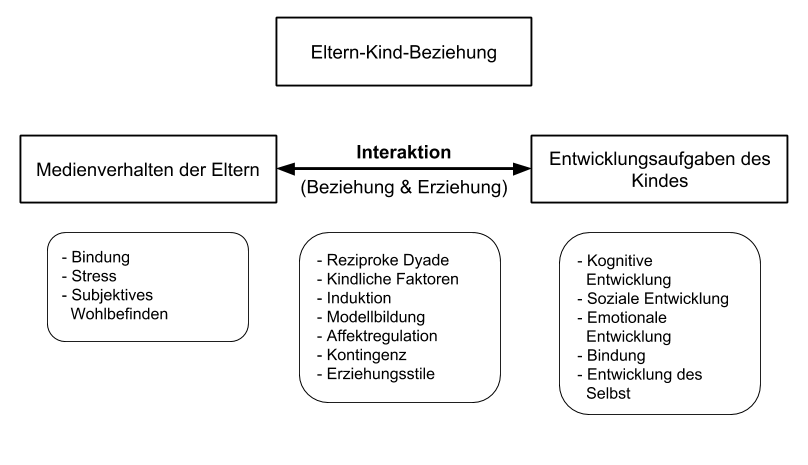
\includegraphics[width=1.0\textwidth]{content/Grafik/Infografik_ElternKindBeziehung_Uebersicht.png}
  \caption{TBD: Infografik: Eltern-Kind-Beziehung}
  \label{fig:InfografikElternKindBeziehung}
\end{figure}

% ---------------------------------------
\subsubsection{Eltern-Kind-Interaktion}\label{sec:Interaktion}
Grundsätzlich ist der Mensch gemäss \citeA[S.~91]{Resch1999} in ein Gefüge von zwischenmenschlichen Relationen eingebettet, welche einen wesentlichen Einfluss auf das innerer Weltverständnis und das Selbstbild nehmen.  Die frühe Kindheit stellt eine kritische Periode in der Entwicklung dar, wobei die wichtigste frühe Umgebung des Kindes die Familie, resp. das primäre Umfeld, ist (vgl. ebd., S. 92ff.). Wird die Familie im Entwicklungskontext angeschaut, so kann der elterliche Einfluss auf das Kind durch die zwei Begriffe \textit{Beziehung} und \textit{Erziehung} definiert werden. Dadurch weist die Eltern-Kind-Beziehung immer Beziehungsqualitäten und Erziehungsqualitäten auf.  

Der Übergang von einer Paargemeinschaft zur Elternschaft führt zu einer grundlegenden Umstrukturierung einer Zweier- zu einer Dreierbeziehung \cite{Hofer1992, Buergin1998}. Dies gelte als eine zentrale Entwicklungsaufgabe von Familien, wobei die Eltern-Kind-Beziehung nicht als einseitige Einflussnahme zu verstehen ist, sondern die Eltern und die Kinder stehen in einer reziproken sozialisatorischen Beziehung zueinander. \citeA{Hofer1992} nennt wichtige Einflussgrössen der dyadischen Beziehung zwischen Vater, Mutter und Kind, die sich auf die kindliche Entwicklung auswirken können: Dabei wird die Synchronizität der Interaktion, die Persönlichkeit der Eltern, die Beziehungsqualität der Partner, sowie die affektive und kognitive Ausstattung des Kindes selbst genannt. 

Auch kindliche Faktoren beeinflussen die frühen Interaktionen deutlich. Das Kind ist schon sehr früh in der Lage, selektiv und adäquat auf die emotionale Ausdrucksform der Bezugsperson einzugehen \cite{Harris1994}. Dabei haben Kinder im Säuglingsalter von der Bezugsperson die Erwartung, dass diese adäquat auf die Gefühlsausdrücke reagiert. Dies ermöglicht bereits dem Säugling einen Informationsaustausch zu seiner Bezugsperson. Somit ist ein Säugling in der Lage, sich anhand dem emotionalen Ausdruck der Bezugsperson anzunähern oder es bleiben zu lassen \cite{Resch1999}. Dieser Vorgang wird als \textit{soziale Vergewisserung (engl. social referencing)} bezeichnet und meint damit, dass ein Kind nach der Beantwortung seiner affektiven Gestimmtheit sucht, wenn es sich seiner Bezugsperson zuwendet. Es konsultiert den Gesichtsausdruck der Bezugsperson, um über die Bedeutung eines ihm unbekannten Ereignisses eine Sinnszuschreibung \textit{(engl. meaning attribution)} zu erhalten. Diese frühen affektiven Regulatoren der Interaktion dienen der Entwicklung des kindlichen Interessens und des kindlichen Bewertungsschemas. Je nach emotionalem Ausutausch wird das Kind eine Kohärenz in seinen Erwartungen entwickeln oder nicht. Wenn die kindlichen emotionalen Signale adäquat beantwortet werden, entsteht eine günstige Basis des Erfahrungslernens \cite[S.~95]{Resch1999}. Die emotionale Kommunikation konstituiert das kindliche Weltbild in Form von Selbst- und Objektrepräsentanzen. Inkonsistente emotionale Kommunikation führt zu einem weniger köhärenten und weniger vorhersagbaren inneren Schemata der Welt. 

Ein weiterer Interaktionsfaktor stellt die \textit{Induktion} aus der empirischen Säuglingsforschung dar. Kindliche Gefühlszustände und Verhaltensmuster werden durch elterliche Verhaltensmuster induziert \cite{Cummings1994}. Intrusive feindliche und unsensitive Elternreaktionen können einen negativen Erregnungsprozess im Kind auslösen, woraus sich ungünstige Interferenzen mit den sich entwickelnden Fähigkeiten des Kindes ergeben, seine eigenen Erregungsimpulse zu modulieren und zu regulieren.  

Über Imitationsprozesse kann die \textit{Modellbildung} im Kind durch das elterliche Verhalten beeinflusst werden. Elterliche Verhaltensweisen und Sichtweisen gegenüber der Welt werden internalisiert \cite{Resch1999}. Die Eltertn ebeeinflussen die Entwicklung des Kindes nicht nur als direkte Akteure, sondern eben auch durch ihre Vorbildfunktion. 

Durch die frühe Interaktion mit einer Bezugsperson wird auch die interaktionelle Affektregulation geprägt. Nach \citeA{Dornes1993, Dornes1997} werden in den frühen Interaktionen zwischen Mutter und Kind affekthaltige Handlungen ausgetauscht. Das Kind kann seine innere Erfahrung mit einem anderen Menschen teilen und mit diesem darüber Kommunizieren. Eine Form dieser affektiven Kommunikation wird gemäss \citeA{Stern1985} als \textit{Affektabstimmung (engl. affective attunement)} bezeichnet. Dabei wird auf bestimmte Gefühlsäusserungen des Kindes von Seiten der Mutter differenziert geantwortet, wobei die Antwort etwas stärker oder schwächer als die des Kindes ausfällt. Durch gezieltes Abdämpfen oder Stimulieren der kindlichen Gefühslausdrücke und Aktionen können Erlebnis- und Handlugsfolgen akzentuiert, abgedämpft oder sogar gelöscht werden. Reagiert eine Bezugsperson unsensibel auf das Kind und werden Handlungsintentionen immer wieder unterbrochen, so kann sich dies negativ auf die Entwicklung des Kindes auswirken \cite{Resch1999}.

Die wechselseitige Bedingtheit des Verhaltens von Menschen wird \textit{Kontingenz} genannt. Gemeint ist dabei die regelhafte Aufeinanderfolge einzelnen Verhaltensschritte. Die Wichtigkeit kontingenter Beantwortung kindlicher Signale, vor allem in der Anfangsphase der Eltern-Kind-Beziehung, betont \citeA{Papousek1987, Papousek1989}. Kontingenz bedeutet dabei die zeitliche und inhaltliche Passung der elterlichen Reaktion auf das Verhalten des Kindes, also die zeitliche Folge der Reaktion und die inhaltliche Entsprechung. Diese frühe Verständigung zwischen Eltern und Kind würde nicht gelingen, wenn die Eltern nicht kompensatorisch an die begrenzte kindlichen Voraussetzungen anpassen würden. Diese Fähigkeit schafft die Voraussetzung für eine gelingende Kommunikation mit dem Säugling im vorsprachlichen Alter. Kontingentes Antworten von Seiten der Eltern ermöglicht eine Kohärenz der Interaktion, die zum subjektiven Gefühl der Kontrolle beim Kind führt.

TBD: Erziehungsstile der Eltern

\subsubsection{Entwicklungsaufgaben der Kinder}\label{sec:Entwicklungsaufgaben}

% ---------------------------------------
\begin{itemize}
    \item Kognitive Entwicklung $\rightarrow$ Umfeld, Vererbung aus \citeA{Berk2011} Kapitel 5.4.2; Seite 224 (Online ZHAW)
    \begin{itemize}
        \item Pos. Korrelation bei Zuneigung und Engagement
        \item schlechte Betreuung S.225 $\rightarrow$ schlechte kognitive Entwicklung
        \item Kommunizieren lernen S.231 / Kap. 5.5 $\rightarrow$ Blickkontakt, Interaktion, viel Unterhaltung förder S. 235, Förderung des frühen Spracherwerbs S.236
    \end{itemize}
    \item Soziale Entwicklung
    \begin{itemize}
        \item Soziale Entwicklung S.469ff \citeA{Siegler2008} (Buch Jeannette)
        \item Soziale Kognition \& Soziale Entwicklung aus \citeA{Bischof2011} S. 237 (Buch von Marc)
    \end{itemize}
    \item Emotionale Entwicklung von Kindern in der Famile aus \citeA{Siegler2008} (Buch Jeannette)
    \begin{itemize}
        \item Qualität Eltern Kind Beziehung S. 561
    \end{itemize}
    \item Bindung aus diversen Quellen
    \begin{itemize}
        \item Bindung und Bindungsverhalten S.98 \citeA{Resch1999} (Buch von Marc)
        \item Bindungstheorie S.583ff \citeA{Siegler2008} (Buch Jeannette)
    \end{itemize}
    \item Die Entwicklungs des Selbst S.274 aus \citeA{Berk2011} (ZHAW Online) 
    \item Erziehungsstile S. 649 aus \citeA{Siegler2008} (Buch Jeannette)
\end{itemize}



% ---------------------------------------
\subsection{TBD: Bindung}\label{sec:Bindung}

% ---------------------------------------
\subsection{TBD: Stress}\label{sec:Stress}

% ---------------------------------------
\subsection{TBD: Subjektives Wohlbefinden}\label{sec:Swb}






% ---------------------------------------
\subsection{TBD: Fragestellung und Hypothesen} \label{sec:Fragestellung}
Die Studie möchte einen möglichen Effekt zwischen dem Bindungsstil der Eltern und deren Medienverhalten während der Betreuung ihrer Kinder untersuchen. Um den Bindungsstil als ausschlaggebende Variable auf das elterliche Medienverhalten zu isolieren, soll der Stress der Eltern als moderierende Variable in die Untesuchung einfliessen.

Welche Auswirkungen das Medienverhalten auf die Eltern haben, soll mittels subjektiven Wohlbefinden  untersucht werden. 

Basierend auf dem oben beschriebenen theoretischen Hintergrund und anhand der aufgezeigten Forschungslücken erschliesst sich die im Folgenden aufgelistete Fragestellung. Basierend auf der Fragestellung wurden die Hypothesen erstellt.
\subsubsection{Fragestellung} 
Welchen Effekt hat der Bindungsstil und das aktuelle Stressempfinden der Eltern auf das im Beisein der Kinder praktizierte Medienverhalten? Kann zwischen diesem elterlichen Verhalten und deren subjektiven Wohlbefinden ein Zusammenhang gefunden werden?
\subsubsection{Hypothese 1}
Eltern mit einem sicheren Bindungsstil weisen eine geringere Mediennutzung im Beisein ihrer Kinder auf als Eltern, die einen unsicher-vermeidenden, unsicher-ambivalenten oder desorganisierten Bindungsstil aufweisen.
\subsubsection{Hypothese 2}
Eltern, die ein hohes Ausmass an Stress empfinden, nutzen Medien im Beisein ihrer Kinder häufiger als Eltern, die ein niedriges Ausmass an Stress aufweisen.
\subsubsection{Hypothese 3}
Eltern mit einem erhöhten Medienverhalten im Beisein ihrer Kinder weisen ein geringeres subjektives Wohlbefinden auf als Eltern, die ein geringeres Medienverhalten im Beisein ihrer Kinder aufweisen.



% Methode
\section{Methode}\label{sec:Methode}
% ---------------------------------------
\subsection{Versuchssituation}\label{sec:Versuchssituation}
Die Durchführung dieser Arbeit erfolgte im Frühlingssemester 2018 im Rahmen einer Masterarbeit an der Zürcher Hochschule für Angewandte Wissenschaften (ZHAW) im Studiengang Angewandte Psychologie in der Vertiefung klinische Psychologie. Dieser Arbeit ging die Wahl des Themas und des Dozenten mittels Disposition im Herbstsemester 2017 voraus. Darin wurde anhand aktueller theoretischer Ansätze und der bisherigen Forschung (siehe auch Kap. \titleref{sec:Hintergrund}) das Vorgehen und das Design vordefiniert und zusammen mit dem betreuenden Dozenten besprochen. 

In einem ersten Schritt wurde, basierend auf der theoretischen Vorarbeit, ein standardisierter Fragebogen anhand der für die Beantwortung der Fragestellung notwendigen Konstrukte \textit{Bindung}, \textit{Stress}, \textit{Medienverhalten} und \textit{subjektives Wohlbefinden}, sowie der soziodemografischen Daten zusammengestellt. Dazu wurden soweit als möglich bereits normierte und validierte Instrumente oder Teile aus bereits existierender Umfragen verwendet. Die Umfrage erfolgte elektronisch über das Internet und setze sich aus einer kurzen Erläuterung der Studie, sowie entsprechende Anweisungen zur Beantwortung der Fragen und den ausgewählten Erhebungsinstrumenten zusammen. 

Die Umsetzung des Fragebogens richtete sich an die von der Umfragesoftware \textit{Enterprise Feedback Suite} der Firma \citeA{Questback2018} vorgegebenen Frageoptionen (ein Auszug des Fragebogens ist in angepasster Form im Anhang \titleref{app:Fragebogen} zu finden). Gestartet wurde die Umfrage mit einer kurzen Einführung, mit der Anonymitätserklärung, dem Hinweis auf den Wettbewerb und die Versuchspersonenstunden. Danach folgten die einzelnen Erhebungsinstrumente, beginnend mit der Erfassung der demographischen Daten, gefolgt vom Mediennutzungs-Fragebogen, dem Bindungsfragebogen, dem Stressfragebogen und dem Fragebogen zum subjektiven Wohlbefinden. Am Ende der Befragung konnten sich die Teilnehmer für die Teilnahme an einem Wettbewerb oder dem Erhalt für Versuchspersonenstunden, wenn sie Studierende der ZHAW in Psychologie waren, entscheiden. Zudem mussten die Teilnehmen angeben, ob sie die Fragen seriös ausgefüllt hatten. Der Fragebogen wurde mittels Pretest auf seine Funktionalität hin überprüft und erfolgte in zwei Schritten. Einerseits erlaubte die Software eine elektronische Testung des Fragebogens auf Korrektheit betreffend der möglichen Antwortpfaden. Dabei ging es um die Auswählbarkeit der Frageoptionen und die Erreichbarkeit aller aufgestellter Frageitems. In einem weiteren Schritt wurden fünf willkürlich ausgewählte Testpersonen aus dem Bekanntenkreis des Autoren als Testpersonen rekrutiert, die den kompletten Umfragebogen durchspieltn. Damit sollte sichergestellt werden, dass die Fragen und deren Anweisungen verständlich formuliert wurden und die Beantwortung der Fragen möglich war. Vor der Aktivschaltung des Fragebogens wurden alle bis dahin erfassten Daten der Tester gelöscht und die gesamte Umfrage frisch initialisiert.

Nach der Fertigstellung der Umfrage wurde diese für die Teilnehmer online verfügbar gemacht. Ab diesem Zeitraum fand die Rekrutierung und die Vorarbeit für die theoretische Auswertung der Resultate statt.

Kurz vor Ende der Umfrage wurde eine Mail an alle an der Rekrutierung involvierten Personen gesandt, um auf das Ende der Umfrage hinzuweisen und ein Dankeschön für die Mithilfe auszusprechen. In diesem Schreiben wurden die Beteiligten darauf hingewiesen, dass sie aufgelgete Flyer entsorgen und geteilte Links entfernen sollen. 

Direkt  nach der Beendingung der Umfrage wurden die Daten bereinigt und in einem Brutto- und Nettodatensatz abgelegt. Es wurden die zum Bezug von Versuchpersonenstunden berechtigte Personen ermittelt und der ZHAW gemeldet. Zudem wurden die Gewinner des Wettberwerbs mittels randomisierter Ziehung gezogen und informiert. Im Anschluss wurden die Daten aufgearbeitet, um die empirischen Hypothesen (siehe Kap. \titleref{sec:EmpirischeHypothesen}) zu prüfen und die Beantwortung der Fragestellung vornehmen zu können.

Die gesamte Arbeit dauerte von der Erstellung der Disposition im Herbstsemester 2017 bis zur Fertigstellung der Masterarbeit Ende Frühlingssemster 2018 zwei Semester und wurde Ende July 2018 zur Bewertung eingereicht.

% ---------------------------------------
\subsection{Design \& Operationalisiserung} \label{sec:Design}
Bei der vorliegenden Studie handelt es sich um eine empirische Querschnitts-Studie mit quantitativem Charakter. Aus ökonomischer Sicht und bezüglich einem hohen Mass an Standardisierung \cite[S.~86ff]{sedlmeier2008} wurde eine schriftliche Befragung via Internet-Fragebogen durchgeführt. Dadurch konnten die Befragten leichter kontaktiert und ein höherer Grad an Anonymität erreicht werden. Dazu wurden die für die Hypothesen relevanten Parameter empirisch erhoben und mittels deskriptiver Statistik ausgewertet. Der Fragebogen wurde in deutscher Sprache verfasst, weshalb die Rekrutierung ausschliesslich in der deutschsprachigen Schweiz erfolgte. Eine Übersetzung der Umfrage in weiter Sprachen hätte den Umfang dieser Arbeit gesprengt, da die einzelnen Fragebögen durch eine der wissenschaft genügenden Hin- und Rückübersetzung durch Personen aus den beiden Muttersprächen zu erfolgen gehabt hätte \cite{Pfetsch2016}.

Im Folgenden werden die einzelnen für die Beantwortung der Fragestellung notwendiger Konstrukte näher erläutert und operationalisiert.

\subsubsection{Soziodemografische Daten}\label{sec:SoziodemografischeDaten}
Bei den soziodemografischen Daten wurden folgende Parameter erfasst: Geschlecht, Jahrgang (Alter), Alter des Kindes in Monaten, Geschlecht des Kindes, brutto Familieneinkommen gemäss \citeA{NZZ2014}, Bildungsabschluss gemäss \citeA{Bfsnd}, Anzahl Personen im gleichen Haushalt, Lebensform, Anzahl Tage, an denen das Kind fremdbetreut ist und der durchschnittliche Betreuungsaufwand pro Woche.

\subsubsection{Medien und Mediennutzung}\label{sec:MedienMediennutzung}
Die Fragebogenitems wurden basierend auf den Vorlagen der Erhebungsinstrumenten der Studien \citeA{Feierabend2017, Blikk2017, Waller2016, Suter2015, Feierabend2015, Kabali2015} neu erstellt. Dabei stand die Mediennutzungszeit während der Betreuung der Kinder, also die Dauer der Mediennutzung in Minuten und das dazu verwendeten Geräte und Medium im Fokus. Es erfolgte ein Spezifizierung des Frageitems hinsichtlich des betreuten Kindes, ob dieses wach war oder geschlafen hat und hinsichtlich des benutzen Mediums, ob dieses privat oder geschäftlich genutzt wurde. Die Erfassung der Mediennutzungszeit wurde anhand der letzten Betreuungstätigkeit vorgenommen, da davon ausgegangen wurde, dass sich die Befragten am ehesten an die absolute Zeit erinnern konnten. Eine Unterteilung in Tage unter der Woche oder am Wochenende wurde als wenig zielführend erachtet. Für die Beantwortung der Fragestellung hätte bereits die reine Mediennutzungszeit gereicht. Es wurde jedoch als hilfreich erachtet, zusätzliche Parameter zu der reinen Mediennutzungsdauer zu erheben, um gegebenenfalls die Fragestellung detaillierter beantworten zu können. Ein weiterer Grund für die zusätzlichen Fragebogenitems ist hinsichtlich der spärlichen Datenlage im Bereich Mediennutzung von Eltern mit Kleinkindern zu nennen. Erfasst wurden neben dem benutzen Medium und der aufgewendeten Zeit, die im Haushalt vorhanden Geräte und auf welches der benutzen Geräte während der Betreuung am wenigsten verzichtet werden konnte. 

\textit{TBD: Operationalisierung - e.g. Gesamtzeit in Minuten, gegliedert nach Medium, etc.}

\subsubsection{Bindung: Adult Attachment Scale (AAS)}\label{sec:AAS}
Für die Erfassung des Bindungsstils (\textit{engl. attachment}) wurde der von \citeA{Schmidt2004} ins Deutsche übersetzte Adult Attachment Scale (AAS) von \citeA{Collins1990} verwendet. Dieser versucht die Bindung über die Selbstbeschreibungsmasse zu erfassen, in Ahnlehnung an die 1-Item-Selbstbeschreibungsmasse von \citeA{Hazan1987}. Dabei gilt dieser gemäss \citeA{Fraley2000} als einer der weit verbreiteten Selbsterfassungsbögen im englischsprachigen Raum.

Der AAS Fragebogen besteht aus insgesamt 18 Items, die auf einer fünfstufigen Likert-Skala von \enquote{stimmt gar nicht} (1), \enquote{stimmt eher nicht} (2), \enquote{stimmt teils / teils} (3), \enquote{stimmt eher} (4) bis \enquote{stimmt genau} (5) eingeschätzt werden. Dabei werden die Skalenwerte als Summenwerte der Itemantworten jeder Skala berechnet. Der Fragebogen bezieht sich auf bindungsrelevante Einstellungen der Befragten und wird mit drei Bindungsskalen erhoben: Die Skala \textit{Nähe} (1) beschreibt das Ausmass, in dem sich eine Person mit Nähe wohl fühlt und diese Nähe nicht mit übermässigen Ängsten verbindet. Die Skala \textit{Vertrauen} (2) beschreibt das Ausmass, in dem eine Person darauf vertraut, dass andere für sie verfügbar sind und dass die Person sich diesen anderen gegebenenfalls tatsächlich anvertrauen kann. Die Skala \textit{Angst} (3) beschreibt in erster Linie Ängste, allein gelassen oder verlassen zu werden. Was sich in einem übermässigen Bedürfnis nach Nähe aus, oder in Befürchtungen, der andere würde diese Bedürnisse zurückweisen. 

Gemäss der Prüfung der Faktorenstruktur des AAS durch \citeA{Schmidt2004} wurden die Elemente 2 und 9 auf Basis der inhaltlichen Ambivalenz der Itemformulierung und der Ergebnisse der konfirmatorischen Faktorenanalyse eliminiert. Diese Reduktion führte zu einer fünf-Item-Version der Skala Nähe und Angst. Die dadurch erhaltene interne Konsistenz (Reliabilität) erreichte in der Untersuchung von \citeA{Schmidt2004} ein $\alpha$ von 0,80 für die Skala Nähe, ein $\alpha$ von 0,72 für die Skala Vertauen und ein $\alpha$ von 0,78 für die Skala Angst. Somit lieferte die überarbeitete Version gemäss \citeA{Buehner2011} niedrige bis mittlere Werte und sind somit zufriedenstellend (Endgültige Version siehe Anhang \titleref{app:AAS}).

Die Operationalisiserung erfolgte anhand der Indizes für die drei Skalen Nähe, Vertrauen und Angst (siehe Formel \titleref{eq:IndexNähe}, \titleref{eq:IndexVertrauen}, \titleref{eq:IndexAngst}). Dabei wurden die Mittelwerte aus den Skalenzugehörigen Items anhand des Likertskalenwerts 1 bis 5 jeder Person berechnet. Zu beachten ist, dass alle Items in der Skala Nähe und die Items $AAS_{5}$, $AAS_{10}$, $AAS_{15}$ und $AAS_{17}$ der Skala Vertrauen für die Erstellung des Skalenwerts umkodiert werden müssen (im Anhang \titleref{app:AAS} mit einem * gekennzeichnet). Je höher die Mittelwerte der Skalen, desto grösser die entsprechende Ausprägung. Tendenziell heisst das bei der Skala Nähe, dass Menschen mit einem hohen Wert, sich bei Nähe zu anderen Menschen eher wohl fühlen. Hohe Ausprägungen bei der Skala Vertrauen geht tendenziell mit einem grösseren Vertrauen anderen Menschen gegenüber einher. Je höher die Werte der Skala Angst, desto eher fürchtet sich ein Mensch alleine gelassen zu werden.
%Formel
\begin{equation}\label{eq:IndexNähe}
    AAS~I_{\text{\textit{N{\"a}he}}}=6-\frac{AAS_{3}+AAS_{8}+AAS_{13}+AAS_{14}+AAS_{18}}{5}
\end{equation}
\begin{equation}\label{eq:IndexVertrauen}
    AAS~I_{Vertrauen}=\frac{AAS_{1}+(6-AAS_{5})+(6-AAS_{10})+AAS_{12}+(6-AAS_{15})+(6-AAS_{17})}{6}
\end{equation}
\begin{equation}\label{eq:IndexAngst}
    AAS~I_{Angst}=\frac{AAS_{4}+AAS_{6}+AAS_{7}+AAS_{11}+AAS_{16}}{5}
\end{equation}

Wie bereits oben beschrieben, lassen sich gemäss \citeA{Schmidt2004} mit dem deutschen Instrument die Bindungsstile nicht direkt zuordnen, sondern in zugrunde liegende Dimensionen einteilen \cite{Schuetzmann2004}. Anhand den Ausprägungen der Probanden in den drei Skalen lassen sich drei Cluster definieren: Im Cluster \textit{sicher} sind Probanden mit hohen Werten bei den Skalen Nähe und Vertrauen und niedrige Werte bei der Skala Angst enthalten. Das Cluster \textit{ängstlich} beinhaltet Probanden mit hohen Werten bei der Skala Angst und mittlere Werte bei den Skalen Nähe und Vertrauen. Im dritten Cluster \textit{vermeidend} befinden sich Probanden, die auf allen drei Skalen Nähe, Vertrauen und Angst tiefe Werte aufweisen.


\subsubsection{Stress: Perceived Stress Questionnaire (PSQ)}\label{sec:PSQ}
Für die Erfassung der aktuellen subjektiv erlebten Belastung, wurde der \textit{Perceived Stress Questionnaire (PSQ)} von \citeA{Levenstein1993} in der deutschen Übersetzung von \citeA{Fliege2001} verwendet.
\citeA{Levenstein1993} kreierte für den anglo-amerikanischen und italienischen Sprachraum ein Instrument, mit dem das Ausmass der subjektiv wahrgenommenen und erlebten aktuellen Belastung erfasst werden soll. Also das Ausmass aktuell wahrgenommener Belastungsfaktoren und das Erleben der eigenen Belastetheit auf der kognitiven und emotionalen Ebene \cite{Fliege2001}. Der Begriff Belastetheit soll verdeutlichen, dass es sich nicht um die Quelle der Belastung, sondern die Reaktion darauf gemeint ist. Die inhaltlichen Kriterien des Fragebogens sind (vgl. ebd.): (1) Stress wird als subjektives Belastungserleben erfasst. Damit wird gemeint, dass sich die Itemformulierung so weit wie möglich an der Perspektive der Wahrnehmung und Bewerung durch die Person orientiert. (2) Belastungsfaktoren und subjektive Belastetheit sollen als übergeordnete Klassen erfasst werden. Dies wird durch eine Vermeiden von Person- und situationsspezifische Formulierungen erreicht (z.B. keine eindeutig berufsbezogene Items). (3) Es wird lediglich das Belastungserleben und nicht der konkrete Umgang mit der Belastung erfragt. Dadurch soll sich der Test von der Erfassung von Bewältigungsbemühungen abgrenzen. Das Belastungserleben wird unabhängig von der Stelle erfasst, an der sich eine Person in einem möglichen Bewältingungsprozess befindet. (4) Es wird die Selbsteinschätzung der Person erhoben und somit nur der bewusste Anteil des Belastungserlebens.

Die Autoren \citeA{Levenstein1993} schlagen vor, das Instrument für Untersuchungen von Zusammenhängen zwischen Stresserleben und Krankheitsentwicklung zu verwenden. Auch wenn in dieser Arbeit weder vom Medienverhalten noch vom subjektiven Wohlbefinden als Krankheit gesprochen werden kann, so sollen die Vorzüge dieses Instruments bezüglich der ökonomisch Durchführbarkeit, die Eignung zur Erfassung möglichst verschiedener Lebenskontexten von Erwachsenen und die Fokussierung auf das gegenwärtige Erleben hervorgehoben werden \cite{Fliege2001}. Bezüglich der empirischen Prüfung und Gütekriterien dieses Testinstruments kann gemäss \citeA{Naescher2009} von einer Auswertungsobjektivität, einer mittleren bis hohen Realiabilität und einer soliden Valildierung ausgegangen werden. Der Perceived Stress Questionnaire \cite{Fliege2001} ist für alle Erwachsenen und für verschiedene Lebenssituationen geeignet. Die deutsche Stichprobe, auf die sich die Werte beziehen, wurde an Probanden zwischen 17 und 79 Jahren erhoben. Der Fragebogen kann gemäss \citeA{Naescher2009} zur Diagnostik des subjektiven Belastungserlebens bei Erwachsenen zweifellos empfohlen werden.

Durch die Validierung und Übersetzung des originalen Fragebogens ins Deutsche, wurden die ursprünglich 30 Items, basierend auf der durchgeführten exploratorischen Faktorenanalyse, auf 20 reduziert. Dadurch entstand die in dieser Arbeit verwendete Kurzversion dieses Fragebogens. Das Verfahren ist im \enquote{Elektronischen Testarchiv} des ZPID enthalten kann für nichtkommerzielle Forschungs- und Unterrichtszwecke kostenlos eingesetzt werden \cite{ZPID}. Ebenso konnten die ursprünglich siebenfaktorielle Zuordnung der Items nicht beibehalten werden. Folgende vier Skalen blieben dabei übrig: (1) Sorgen, (2) Anspannung, (3) Freude und (4) Anforderungen. Diese Veränderungen sind nachvollziehbar und bei \citeA{Fliege2001} ausführlich dokumentiert. Die Einschätzung erfolgt über eine viertstufige Likertskale, die von 1 für \textit{fast nie}, über 2 für \textit{manchmal}, 3 für \textit{häufig} bis zu 4 für \textit{meistens} reicht. Bei den Items handelt es sich um Feststellungen, die von der Testperson beurteilt werden sollen (siehe dazu auch Anhang \titleref{app:PSQ}. 

Die Operationalisierung erfolgte anhand der Anleitung von \citeA{Naescher2009}. Dabei wurden die Indizes der vier Skalen Sorgen, Anspannung, Freude und Anforderungen mit Hilfe der Mittelwertsbildung erstellt (siehe \titleref{eq:PSQIndexSorgen}, \titleref{eq:PSQIndexAnspannung}, \titleref{eq:PSQIndexFreude} und \titleref{eq:PSQIndexAnforderung}). Dazu werden die jeweiligen Items der zugehörigen Skala aufaddiert und durch deren Anzahl dividiert. Hohe Werte in einer Skala bedeuten jeweils auch eine hohe Ausprägung der betreffenden Eigenschaft.

%Formel
\begin{equation}\label{eq:PSQIndexSorgen}
    PSQ~I_{Sorgen}=\frac{\frac{PSQ_{05}+PSQ_{07}+PSQ_{10}+PSQ_{13}+PSQ_{15}}{5}-1}{3}*100
\end{equation}
\begin{equation}\label{eq:PSQIndexAnspannung}
    PSQ~I_{Anspannung}=\frac{\frac{(5-PSQ_{01})+(5-PSQ_{06})+PSQ_{09}+PSQ_{17}+PSQ_{18}}{5}-1}{3}*100
\end{equation}
\begin{equation}\label{eq:PSQIndexFreude}
    PSQ~I_{Freude}=\frac{\frac{PSQ_{04}+PSQ_{08}+PSQ_{12}+PSQ_{14}+PSQ_{16}}{5}-1}{3}*100
\end{equation}
\begin{equation}\label{eq:PSQIndexAnforderung}
    PSQ~I_{Anforderung}=\frac{\frac{PSQ_{02}+PSQ_{03}+PSQ_{11}+(5-PSQ_{19})+PSQ_{20}}{5}-1}{3}*100
\end{equation}

Zu beachten ist, dass gewisse Items für die Berechnung der Indizes umkodiert werden müssen. Hierbei handelt es sich um die drei Items $PSQ_{01}$, $PSQ_{06}$ und $PSQ_{19}$ (im Anhang \titleref{app:PSQ} mit einem * gekennzeichnet).

Zudem wird von \citeA{Naescher2009} eine Skalenrange-Transformation von 0 bis 100 vorgeschlagen. Dazu wird aus dem Mittelwert der Skala mit dem Skalenranges von 1 bis 4 durch Subtraktion von 1 eine lineare Transformation zu 0 bis 3 vorgenommen. Die weitere lineare Transformation mittels Division durch 3 ergibt einen Wert zwischen 0 und 1, welcher multipliziert mit 100 ein Skalenrange zwischen 0 und 100 ergibt.  

Für den Gesamtscore muss die Skala Freude umkodiert werden:

%Formel
\begin{equation}\label{eq:PSQGesamtscore}
    PSQ~I_{Gesamtscore}=\frac{PSQ~I_{Sorgen}+PSQ~I_{Anspannung}+ (100-PSQ~I_{Freude})+PSQ~I_{Anforderung}}{4}
\end{equation}

In den Gesamtscore fliessen die oben berechneten Skalen ein und ergeben das allgemeine Stresserleben, respektive die aktuelle, subjektiv erlebte Belastung einer Person.

\subsubsection{Subjektives Wohlbefinden: Subjective Happiness Scale (SHS)}\label{sec:SWB}
Die Erfassung des subjektiven Wohlbefindens erfolgte anhand dem von \citeA{Lyubomirsky1999} entwickelten \textit{Subjective Happiness Scale (SHS)}, in der deutschen Übersetzung und Überprüfung von \citeA{Swami2009}. Der SHS wurde für die Erfassung  eines allgemeinen subjektiven Wohlbefindens mittels Selbtseinschätzungsfragebogen entwickelt. Ein Wohlbefinden, dass in seiner globalen und grundsätzlichen Ausprägung, also ob es sich um einen glücklichen oder unglücklichen Menschen handelt, erfasst wird  \cite[S.~139ff]{Lyubomirsky1999}. Die Skala enthält insgesamt vier Items. Zwei davon erfassen das eigene Selbstbild, basierend auf einer absoluten Einschätzung des eigenen Wohlbefindens und einer Einschätzung verglichen mit dem eigenen sozialen Umfeld. Bei den weiteren beiden Items wird die befragte Person angehalten, sich bezüglich einer individuellen Beschreibungen glücklicher und unglücklicher Menschen einzuschätzen. Das Antwortformat der vier Items basiert auf einer sieben Punkte Likertskala (z.B.: 1 für \textit{Kein glücklicher Mensch} bis 7 \textit{Sehr glücklicher Mensch}). 

\citeA{Lyubomirsky1999} weisen darauf hin, dass der SHS sich für die Erfassung des subjektiven Wohlbefindens besser eignet als andere vergleichbare Instrumente (z.B.: \textit{Affect Balance Scale} oder \textit{the Satisfaction With Life Scale}), da der Fragebogen eine globale subjektive Einschätzung bezügliche Wohlbefinden vornimmt, im Gegensatz zur Erfassung von eigentlichen Glückszuständen, die einer bestimmte Zeitspanne zuzuordnen sind (z.B.: affektive und kognitive Zustände). Der Fragebogen wurde in 14 Studien mit einem Total von 2,732 Teilnehmern validiert. Die Daten wurden innerhalb der vereinigten Staaten anhand von Studenten zweier Universitäten und einer Mittelschule, von Erwachsenen innerhalb zweier Städten in Kalifornien   erhoben. Zudem wurden Teilnehmer aus Moswkau, Russland beigezogen. Demzufolge soll der SHS eine hohe interne Konsistenz aufweisen, welche über alle Stichproben stabil blieben. Die Test-Retest-Korrelation und die Korrelation zwischen Eigen- und Fremdeinschätzung deuten auf eine gute bis sehr gute Realiabilität hin. 
Zudem deute die Konstruktvalidität darauf hin, dass der Fragebogen auch wirklich das Konstrukt subjektives Wohlbefinden misst (vgl. ebd.). \citeA{Swami2009} konnten in ihrer Studie nachweisen, dass es sich bei der deutschen Übersetzung um eine unidimensionale Struktur, mit einer hohen internen Konsitenz handelt. Diese Übersetzung korrelierte hoch mit anderen Messinstrumenten, welche das subjektive Wohlbefinden erfassen. Demzufolge habe der neue Fragebogen eine gute Konvergenzvalidität. Hingegen konnten die Forscher keine Aussage über die Test-Retest-Reliabilität machen, noch nahmen sie eine Validierungsprüfung vor, da dies nicht zum Gegenstand ihrer Überprüfung zählte (vgl. ebd.).

Die Operationalisierung erfolgt anhand der Mittelwertsbildung der vier Items \cite{Lyubomirsky1999} und ergibt einen SHS-Index (siehe \titleref{eq:SHS}). Die mögliche Ausprägung dieses Index reicht von 1.0 bis 7.0. Eine hohe Ausprägung steht für ein hohe subjektive Zufriedenheit.

%Formel
\begin{equation}\label{eq:SHS}
    SHS~I=\frac{SHS_{1}+SHS_{2}+SHS_{3}+SHS_{4}}{4}
\end{equation}

\subsection{Datenerhebung \& Rekrutierung}
Zur Datengewinnung wurde die von der ZHAW zur Verfügung gestellten Umfragesoftware Enterprise Feedback Suite in der Version 10.9 der Firma \citeA{Questback2018} verwendet. Der Fragebogen wurde mit Hilfe der zur Verfügung gestellten Dokumentation kreiert \cite{EFS2016} und wurde Mitte Januar bis Ende Mai 2018 aktiv geschaltet.  Der Zugang zur Befragung erfolgte über die von der Firma \citeA{Questback2018} zur Verfügung gestellten öffentlichen Internetadresse, welche zum Zeitpunkt der Befragung wie folgt lautete: https://ww2.unipark.de/uc/elternfragebogen/.

Die Rekrutierung erfolgte im Sinne einer Gelegenheitsstichprobe, da das Ziel dieser Untersuchungen in der Erfassung der Veränderung der abhängigen Varibalen Mediennutzung anhand der unabhängigen Variablen Bindung und Stress ist und sich dieses Vorgehen als ökonomisch und praktikabel im Hinblick auf die Forschungsfrage herausstellte \cite{TUDresden2015}. Für den Versand der Umfrage wurde ein Infomail und ein Infozettel (Flyer) mit den wichtigsten Angabe zur Studie und dem Link zur Umfrage erstellt (siehe dazu \titleref{app:Mailing} und \titleref{app:Flyer} im Anhang). Der Flyer wurde zusätzlich in Papierform ausgedruckt. Für den Versand des Flyers und des Infomailings wurden unterschiedliche Kanäle verwendet: Einerseits wurden diese per Post für die jeweilige Auslage und den Aushang versendet, andererseits erfolgte der Versand elektronisch über Mail, Facebook-Posting und Text-Nachrichten. Zudem wurde der Flyer auf unterschiedlichen einschlägigen Webseiten publiziert. Um den Medienbruch möglichst gering zu halten, wurde wann immer möglich versucht, den Link für die Umfrage elektronisch zugänglich zu machen. 

Die Rekrutierung fand an folgenden Orten und Institutionen statt (für eine detaillierte Übersicht, siehe Anhang \titleref{app:Rekrutierung}): Direkt an der ZHAW, über die Elternberatungsstellen der deutschsprachigen Schweiz \cite{Sfmvb2018}, über Spitäler mit Wochenbett und Kinderärzte, über die deutschsprachigen Familienzentren \cite{NetzwerkBildung2018}, über die Anschrift aller deutschsprachiger Niederlassungen der \citeA{Elternbildung2018} und über das private Umfeld des Autors, mit der Bitte, die Umfrage im eigenen Umkreis weiter zu verteilen. Zudem wurde die Umfrage auf der Internetplattform der Elternzeitschrift \enquote{Fritz \&  Fränzi}, dem Marktplatz des Elternmagazins \enquote{Wir Eltern} und dem Forum der Internetplattform \enquote{Swissmom} publiziert.

\textit{TBD: Anreiz} Wettbewerb und VPN Stunden...

\subsection{Beschreibung der Stichprobe}
Insgesamt schlossen brutto 248 Personen die Umfrage ab. 1454 Personen sind zumindest auf die erste Seite gekommen und haben anschliessend abgebrochen. Dies entspricht einer Beendingungsquote von 17.06\%. Die meisten Abbrüche sind auf der Startseite mit 1045 zu verzeichnen (71.87\%), gefolgt von den demografischen Daten mit 100 (6.88\%) und Medien und Mediennutzung mit 44 (3\%). Die mittlere Bearbeitungszeit des Fragebogens dauerte 27 Minuten. 

Nach der Datenbereinigung blieben netto 218 Personen übrig (87.9\%). Eine Personen wurde ausgemustert, da sie beim Jahrgang einen fehlerhaften Wert angegeben hatte (Jg 2017). Zwei weitere Person gaben an, die Umfrage nicht seriös ausgefüllt zu haben. Zwei Personen mussten entfernt werden, da die Personen bei der Angabe der Mediennutzungszeit in Minuten mit Ja und Nein geantwortet haben. 25 Personen wurden entfernt, da das Alter ihrer Kinder 13 Monate überstieg. 

Die Merkmale Geschlecht, Alter in Jahren, Geschlecht Kind und Alter Kind in Jahren werden in Tabelle \titleref{table:Stichprobe} dargestellt (eine um die Merkmale Familieneinkommen, Bidlungsabschluss, Anzahl Personen im Haushalt, Lebensfrom und Fremdbeteruung in Tagen ist in Anhang \titleref{app:Gesamtstichprobe} zu finden).

\begin{table}[htbp]

\begin{tabular}{m{0.5em}  m{10em}  m{5em}} 
  \hline\hline
  \multicolumn{2}{l}{\textbf{Merkmal}} & \textbf{$n$ (\%)} \\
  \hline
  \multicolumn{2}{l}{Geschlecht} \\ 
   & weiblich & 198 (90.8)\\ 
   & männlich & 19 (8.7)\\ 
   & keine Angabe & 1 (.5)\\ 
   
  \multicolumn{2}{l}{Alter in Jahren} \\
   & $M$ (Min./Max.) & 33.9 (20/48) \\
   & $SD$ & 4.5 \\
  
  \multicolumn{2}{l}{Geschlecht Kind} \\
   & weiblich & 97 (44.5)\\ 
   & männlich & 119 (54.6)\\ 
   & keine Angabe & 2 (.9)\\
  
  \multicolumn{2}{l}{Alter Kind in Monaten} \\
   &  $M$ (Min./Max.) & 6.6 (0/12)\\
   & $SD$ & 3.4\\
  \hline\hline
  &&\\
\end{tabular}
\caption{Stichprobe}
\label{table:Stichprobe}
\end{table}

Das Alter der Befragten liegt zwischen 20 und 48 Jahre mit einem Durchschnittsalter von 33.9 Jahren ($SD$ = 4.5). Weibliche Probanden sind mit 90.8 \% ($n$ = 198) in der Stichprobe vertreten. Das Geschlecht der Kinder ist mit 44.5\% weiblichen ($n$ = 97) und 54.6\% männlichen ($n$ = 119) Kindern vertreten. Das Alter der Kinder liegt zwischen 0 und 12 Monaten mit einem Durchschnitt von 6.6 Monaten ($SD$ = 3.4).

Bei der Angabe zum Familieneinkommen (siehe Tabelle \titleref{table:Gesamtstichprobe} im Anhang \titleref{app:Gesamtstichprobe}) zeigt sich die stärkste Ausprägung bei Personen, die über ein Familieneinkommen von über CHF 104'001 und mehr verfügen mit 34.3\% ($n$ = 75), gefolgt von Familien mit einem Einkommen zwischen CHF 78'001 und CHF 104'000 mit 30.3\% ($n$ = 66) und Familien mit einem Einkommen zwischen CHF 52'000 und CHF 78'000 mit 23.9\% ($n$ = 52). 

73 Personen gaben an über ein Uni oder Fachhochschultitel zu verfügen, was mit 33.5\% die höchste Ausprägung darstellt, dicht gefolgt von einem Lehrabschluss mit 23.9\% ($n$ = 52) und einem Abschluss an einer höheren Fachschule mit 22.9\% ($n$ = 50). Zusammenfassend ergibt das einen Abschluss im tertiären Bereich von 60.6\% ($n$ = 132), im Sekundar II Bereich von 36.6\% ($n$ = 79) und im Bereich der Grundschule 2.8\% ($n$ = 6).

Im Durchschnitt leben zwischen 2 und 8 Personen im Haushalt mit einem Durchschnitt von 3.6 Personen ($SD$ = .8). Die dominante Lebensform stellt die verheiratete Partnerschaft mit 71.6\% ($n$ = 156) dar, gefolgt von der nicht verheirateten Partnerschaft mit 25.2\% ($n$ = 55). Die Kinder werden im Schnitt 1 Tag ($SD$ = 1.3)  zwischen 0 und 5 Tagen fremd betreut.

\subsection{Empirische Hypothesen}\label{sec:EmpirischeHypothesen}
\subsection{Statistische Analyseverfahren}

% Ergebnisse
\section{Ergebnisse}\label{sec:Ergebnisse}
\subsection{Vorbereitung der Daten und deskriptive Analysen}
Die erhobenen Daten wurden mittels SPSS Version 25 für Mac OS X aufbereitet. Die Stichprobendaten wurden direkt aus der \acrfull{efs} \cite{Questback2018} mittels Datenexport für SPSS exportiert. Allfällige Fehlerquellen wurden bei der Datenbereinigung korrigiert. Dies wurde durch \acrshort{efs} erleichtert, indem nur abgeschlossene Datensätze exportiert wurden und eine erste Werteprüfung bereits bei der Eingabe erfolgte (z.B.: wurden nur Zahlen bei der Eingabe des Jahrgangs zugelassen). Fehlende Eingaben durch die Teilnehmenden wurden durch vordefinierte Werte von \acrshort{efs} gesetzt. Dadurch wurden diese \enquote{Missing-Values} innerhalb von SPSS als solche berücksichtigt und flossen als fehlende Datenwerte in die Berechnungen ein. Für die Berechnung der \enquote{Mediennutzung}, der \enquote{Bindung}, des \enquote{Stressniveaus} und des \enquote{subjektiven Wohlbefindens} wurden zusätzliche Variablen in SPSS erstellt und basierend auf Skalenwerten der Teilnehmenden berechnet (für die Formel der Berechnung siehe Sektion \textit{\nameref{sec:Design}}).

\subsubsection{Medien und Mediennutzung}
Im Rahmen der Umfrage wurde die Mediennutzung während der Betreuung der Kinder erhoben. Dabei wurde zwischen \enquote{privat genutzt}, \enquote{geschäftlich genutzt}, \enquote{privat \& geschäftlich genutzt} und \enquote{nicht genutzt} unterschieden. In Folge der Übersichtlichkeit wurde in Abbildung \ref{fig:Mediennutzung}, S. \pageref{fig:Mediennutzung} die Ausprägung auf \textit{genutzt} und \textit{nicht genutzt} zusammengefasst, wobei die geschäftliche und die private Nutzung zusammengefasst wurde (für eine detaillierte Darstellung siehe Anhang \ref{app:Mediennutzung}, Abbildung \ref{fig:AppMediennutzung}).

% Figure
\begin{figure}[hbt]
\caption{Medien \& Mediennutzung}\label{fig:Mediennutzung}
\centering
\begin{tikzpicture}[scale=1, auto,swap]
  \begin{axis}[
    xbar stacked,
    %y axis line style = { opacity = 0 },
    %axis x line       = none,
    tickwidth         = 0pt,
    xmin              = 0,
    xmax              = 105,
    enlarge y limits  = 0.1,
    enlarge x limits  = 0.02,
    %/legend pos=south east,
    legend style={at={(0.5,-0.13)}, anchor = north},
    legend columns     = -1,
    %reverse legend,
    ytick             = data,
    xlabel            = {Mediennutzung (\textit{Angaben in \%})},
    %height            = 20cm,
    width             = 14cm,
    symbolic y coords = {MP3, Spielkonsole, Fotokamera, Printmedien, Radio, Tablet, Computer, TV, Smartphone},
    nodes near coords,
    nodes near coords align={horizontal},
  ]
  %benutzt
  \addplot[draw=black,fill=cyan] coordinates { (97.2,Smartphone)(31.7,TV)(42.2,Computer)(19.7,Tablet)(62.8,Radio)(68.8,Printmedien)(55,Fotokamera)(4.1,Spielkonsole)(8.3,MP3)};
  \addlegendentry{genutzt~}
  %nicht genutzt
  \addplot[draw=black,fill=orange] coordinates { (2.8,Smartphone)(68.3,TV)(57.8,Computer)(80.3,Tablet)(37.2,Radio)(31.2,Printmedien)(45,Fotokamera)(95.9,Spielkonsole)(91.7,MP3)};
  \addlegendentry{nicht genutzt}
  
  \end{axis}
\end{tikzpicture}
\end{figure}

97.2\% der Befragten gaben an, das Smartphone während der Betreuung ihrer Kinder zu benutzen, wobei dies zu 72\% privat, 1.4\% geschäftlich und zu 23.9\% privat \& geschäftlich erfolgte. 2.8\% benutzte das Smartphone während der Betreuung nicht. 31.7\% gaben an, den Fernseher während der Betreuung ihrer Kinder privat zu nutzen und 68.3\% gaben an, den Fernseher nicht zu nutzen. Den Computer (Laptop- oder Desktopcomputer) nutzten 42.4\% während Betreuungszeiten, unterteilt in 17.4\% privat, 6.4\% geschäftlich und 18.3\% privat \& geschäftlich. 57.8\% nutzte keinen Computer während der Betreuung. Das Tablet nutzten 19.7\% während der Betreuung (17\% privat, 0\% geschäftlich und 2.8\% privat \& geschäftlich). 80.3\% nutzten das Tablet während dieser Zeit nicht. Den Radio (Stereoanlage, CD Player) nutzten 62.8\% während der Betreuung ihrer Kinder hauptsächlich privat (57.3\% privat, 1.4\% geschäftlich, 4.1\% privat \& geschäftlich). 37.2\% nutzte den Radio nicht. Printmedien (Buch, Zeitung, Heft, Comic) wurden von 68.8\% der Eltern während der Zeit mit ihren Kindern genutzt (58.7\% privat, 1.8\% geschäftlich und 8.3\% privat \& geschäftlich) und von 31.2\% nicht genutzt. Foto- oder Videokamera nutzten 55\%, wobei der Hauptanteil von 51.8\% im privaten Rahmen stattfand (0\% geschäftlich und 3.2\% privat \& geschäftlich). Die Spielekonsole wurde währen der Betreuung von 4.1\% privat genutzt, gegenüber 95.9\%, die sie nicht benutzte. Der MP3 Player wurde von 8.3\% genutzt, unterteilt in 7.3\% private, 0\% geschäftliche und 0.9\% private \& geschäftliche Nutzung. 91.7\% nutzte den MP3 Player nicht während der Betreuung.

Weiter wurde die Medientätigkeit in Minuten anhand der letzten Betreuung des Kindes erfasst (siehe Tabelle \ref{table:Medientätigkeit}, S. \pageref{table:Medientätigkeit}). Dabei wurde unterschieden, ob das Kind wach war $MNS_{Wach}$ oder geschlafen hat $MNS_{Schlafend}$. Alle Medientätigkeiten summiert ergaben den Mittelwert der Mediennutzung. Dieser belief sich währendem das Kind wach war auf $M$ = 93.1 Minuten ($SD$ = 103.6, $Min$ = 0, $Max$ = 613) und $M$ = 108.6 Minuten, währendem das Kind geschlafen hat ($SD$ = 105.3, $Min$ = 0, $Max$ = 495). Total waren die Teilnehmer im Schnitt $M$ = 202.1 Minuten mit Medien beschäftigt, währendem sie ihr Kind betreuten ($SD$ = 174.9, $Min$ = 3, $Max$ = 840).

%Table
\begin{table}[b]
\begin{tabular}{m{8em} m{4em}  m{4em}  m{5em} m{4em}} 
  \hline
  & $M$ & $SD$ & Min - Max & Schiefe\\
  \hline
  $MNS_{Wach}$* & 93.08 & 103.61 & 0 - 613 & 2.26\\
  $MNS_{Schlafend}$** & 108.63 & 105.32 & 0 - 495 & 1.56\\
  $MNS_{Total}$*** & 202.10 & 174.86 & 3 - 840 & 1.44 \\
  \hline
  \multicolumn{5}{l}{\textit{Anmerkung. *$N$ = 208, **$N$ = 205, ***$N$ = 204, Angaben in Minuten.}}\\
  &&&&\\
\end{tabular}
\caption{Medientätigkeit während der Betreuung}
\label{table:Medientätigkeit}
\end{table}

Auf die einzelnen Medien verteilt bedeutet das, dass die Probanden im Schnitt $M_{w}$ = 5.2 Minuten telefonierten, während dem das Kind wach war und $M_{s}$ = 7.2 Minuten, währendem das Kind geschlafen hat (siehe dazu Abbildung \ref{fig:Medientätigkeit}). Im Schnitt haben die Teilnehmer $M_{w}$ = 10 Minuten mit Textnachrichten verbracht (Lesen und Schreiben) währendem das Kind war wach und $M_{s}$ = 13.8 Minuten währendem das Kind geschlafen hat. Für das Bearbeiten und Lesen von Emails setzten die Teilnehmenden $M_{w}$ = 1.7 Minuten (Kind war wach) und $M_{s}$ = 7 Minuten ein (Kind hat geschlafen). Beim Lesen und Anschauen von Printemedien ((Bilder-)Bücher, Magazinen, Zeitungen, Comics, etc.) setzten die Eltern $M_{w}$ = 5.3 und $M_{s}$ = 12.5 Minuten ein. Im Internet verbrachten sie $M_{w}$ = 5.9 und $M_{s}$ = 19.7 Minuten mit Surfen und Informationen suchen. Musik hörten die Eltern während der Betreuung $M_{w}$ = 18.6 und $M_{s}$ = 8.3 Minuten. Sie schauten im Schnitt $M_{w}$ = 5.4 und $M_{s}$ = 25.1 Minuten Fernsehen oder Videos (TV-Sender, Netflix, DVD, etc.). Der Radio lief während $M_{w}$ = 34.3 und $M_{s}$ = 12.9 Minuten. Fotos oder Videos wurden während $M_{w}$ = 5.1 und $M_{s}$ = 0.9 Minuten gemacht. Video-Games (Smartphone, Computer, Konsole, etc.) wurden während $M_{w}$ = .2 und $M_{s}$ = 1.5 Minuten gespielt. Hörspiele und Hörbücher wurden während $M_{w}$ = 1.5 und $M_{s}$ = 2.1 Minuten gehört. Die komplette Auflistung der Mittelwerte (wach \& schlafend), inklusive Angabe des  Mittelwerts ist in Tabelle \ref{fig:AppMedientätigkeit} im Anhang zu finden.

\begin{figure}%[htp]
\caption{Mittelwerte der Medientätigkeiten während der Betreuung}\label{fig:Medientätigkeit}
%\centering
\begin{tikzpicture}[scale=1]
  \begin{axis}[
    xbar stacked,
    %y axis line style = { opacity = 0 },
    %axis x line       = none,
    tickwidth         = 0pt,
    xmin              = 0,
    xmax              = 47,
    enlarge y limits  = 0.08,
    enlarge x limits  = 0.02,
    legend pos=south east,
    ytick             = data,
    xlabel            = {Mittelwerte $M$ (\textit{Angaben in Minuten})},
    %height            = 20cm,
    width             = 13cm,
    symbolic y coords = {Hörspiele, VideoGames, Fotos, Radio, TV, Musik, Internet, Lesen, Email, SMS, Telefonieren},
    nodes near coords,
    nodes near coords align={horizontal},
  ]
  %wach
  \addplot[draw=black,fill=cyan] coordinates { (5.2,Telefonieren)(10,SMS)(1.7,Email)(5.3,Lesen)(5.9,Internet)(18.6,Musik)(5.4,TV)(34.3,Radio)(5.1,Fotos)(.2,VideoGames)(1.5,Hörspiele)};
  
  %schlafend
  \addplot[draw=black,fill=orange] coordinates { (7.2,Telefonieren)(13.8,SMS)(7,Email)(12.5,Lesen)(19.7,Internet)(8.3,Musik)(25.1,TV)(12.9,Radio)(0.9,Fotos)(1.5,VideoGames)(2.1,Hörspiele)};
  
  \legend{\text{$M$ Kind wach}, \text{$M$ Kind schlafend}}
  \end{axis}
\end{tikzpicture}
\end{figure}

Neben der Mediennutzung und der Medientätigkeit wurde die Anzahl Geräte im Haushalt erfragt (detaillierte Auflistung siehe Tabelle \ref{fig:AppGeräteHaushalt} im Anhang). Dabei gaben 83.9\% der Teilnehmer an, zwei Smartphones im Haushalt zu besitzen. 70.2\% gaben an, ein TV-Gerät zu besitzen. 45\% der Befragten besitzen zwei Computer (Desktop oder Laptop), 45.9\% ein Tablet und 48.2\% einen Radio (Stereoanlage, CD-Player) im Haushalt. 51.4\% gaben an, keine Tageszeitung oder ein Magazine abonniert zu haben. 45.9\% gaben an, einen Fotoapparat oder Videokamera zu besitzen. 61\% besitzen keine Spielekonsole und 67\% keinen MP3 Player.

Zudem wurden die Medien erhoben, auf welche die Eltern während der Betreuung am wenigsten verzichten konnten (siehe Tabelle \ref{fig:AppMedienverzicht} im Anhang). 85.3\% gaben an, nicht auf das Smartphone verzichten zu können, gefolgt von Radio 33.9\% (Stereoanlage, CD-Player) und 25.2\% Foto- und Videokamera. Weiter gaben die Teilnehmer an, dass 11.9\% von ihnen nicht auf den Fernseher, 9.6\% nicht auf das Abonnement einer Tageszeitung oder Zeitschrift, 8.3\% nicht auf den Computer (Laptop oder Desktop), 2.8\% nicht auf den MP3-Player, 2.3\% nicht auf das Tablet und .9\% nicht auf die Spielekonsole verzichten können.

\subsubsection{Bindung anhand AAS}
Die Skalenauswertung der \acrfull{aas} lieferte weitere Werte (siehe Tabelle \ref{table:AASDeskriptivTrans}). Dabei wurden die transformierten Skalen mit einem Wertebereich von 0 bis 100 verwendet (siehe dazu Formel \ref{eq:AASIndexTrans} in Kapitel \textit{\nameref{sec:AAS}}). Der Mittelwert $M$ der Skala $AAS_{\textnormal{Nähe}}$ beträgt 78.46 ($SD$ = 15.98). Der Mittelwert $M$ der Skala $AAS_{Vertrauen}$ beträgt 80.18 ($SD$ = 16.98) und der Mittelwert  $M$ der Skala $AAS_{Angst}$ beträgt 20.28 ($SD$ = 17.43). Die entsprechenden Werte der originalen Skalen sind in Tabelle \ref{table:AppAASDeskriptiv} im Anhang zu finden.

%Table
\begin{table}%[ht]
\begin{tabular}{m{7em} m{3em}  m{3em}  m{5em} m{3em}} 
  \hline
  & $M$ & $SD$ & Min - Max & Schiefe\\
  \hline
  $AAS_{\textit{\textnormal{NäheTrans}}}$ & 78.46 & 15.98 & 25 - 100 & -.59\\
  $AAS_{VertrauenTrans}$ & 80.18 & 16.98 & 16.67 - 100 & -1.17\\
  $AAS_{AngstTrans}$ & 20.28 & 17.43 & -5 - 75 & .91 \\
  \hline
  \multicolumn{5}{l}{\textit{Anmerkung. $N$ = 217, Wertebereich Skala 0 bis 100.}}\\
  &&&&\\
\end{tabular}
\caption{Transformierte Skalenwerte der Adult Attachment Scale - AAS}
\label{table:AASDeskriptivTrans}
\end{table}

Für die Beantwortung der Fragestellung wurde anhand der Skalen eine Aufteilung der Stichprobe in \enquote{sicher} und \enquote{unsicher} gebundene Personen vorgenommen. Wie bereits in Kapitel \textit{\nameref{sec:AAS}} beschrieben, kann eine Aufteilung in das Cluster \enquote{sicher} vorgenommen werden \cite{Schuetzmann2004}. Gemäss dieser Aufteilung lassen sich 69.7\% ($N$ = 144) der Probanden als sicher und 30.3\% ($N$ = 60) als unsicher gebundene Personen einteilen. 

\subsubsection{Stress anhand \acrshort{psq}}
Die Skalenauswertung des \acrfull{psq} liefert folgende Werte (siehe Tabelle \ref{table:PSQDeskriptiv}). Der Mittelwert $M$ der Skala $PSQ_{Sorgen}$ beträgt 24.28 ($SD$ = 17.69). Der Mittelwert $M$ der Skala $PSQ_{Anspannung}$ beträgt 42.14 ($SD$ = 21.96). Der Mittelwert $M$ der Skala $PSQ_{Freude}$ beträgt 65.26 ($SD$ = 19.08). Der Mittelwert $M$ der Skala $PSQ_{Anforderung}$ beträgt 46.97 ($SD$ = 19.54) und der Gesamtmittelwert $M$ der Skala $PSQ_{Gesamtscore}$ beträgt 37.03 ($SD$ = 17.11).

%Table
\begin{table}[ht]
\begin{tabular}{m{6em} m{3em}  m{3em}  m{5em} m{3em}} 
  \hline
  & $M$ & $SD$ & Min - Max & Schiefe\\
  \hline
  $PSQ_{Sorgen}$ & 24.28 & 17.69 & 0 - 86.67 & .84 \\
  $PSQ_{Anspannung}$ & 42.14 & 21.96 & 0 - 100 & .26\\
  $PSQ_{Freude}$ & 65.26 & 19.08 & 6.67 - 100 & -.14\\
  $PSQ_{Anforderung}$ & 46.97 & 19.54 & 0 - 100 & .37 \\
  $PSQ_{Gesamtscore}$ & 37.03 & 17.11 & 3.33 - 91.67 & .42\\
  \hline
  \multicolumn{5}{l}{\textit{Anmerkung.} $N$=218, Skala Wertebereich 0 bis 100}\\
  &&&&\\
\end{tabular}
\caption{Skalenwerte des Perceived Stress Questionnaire - PSQ}
\label{table:PSQDeskriptiv}
\end{table}


\subsubsection{Wohlbefinden anhand \acrshort{shs}}
Der Indexwert der \acrfull{shs} $SHS~I$ beläuft sich in dieser Stichprobe auf $M$ 5.53 ($SD$ = 1.01) (siehe Tabelle \ref{table:SHSDeskriptiv}).

%Table
\begin{table}[ht]
\begin{tabular}{m{6em} m{3em}  m{3em}  m{5em} m{3em}} 
  \hline
  & $M$ & $SD$ & Min - Max & Schiefe\\
  \hline
  $SHS~I$ & 5.53 & 1.01 & 2.25 - 7.0 & -.77 \\
  \hline
  \multicolumn{5}{l}{\textit{Anmerkung.} $N$ = 218, Skala Wertebereich 1 bis 7}\\
  &&&&\\
\end{tabular}
\caption{Skalenwerte des Subjective Happiness Scale - SHS}
\label{table:SHSDeskriptiv}
\end{table}

% ---------------------------------------
\subsection{Hypothesentest} \label{sec:Hypothesentest}
In diesem Kapitel werden die Hypothesen eins bis vier der Reihe nach geprüft (für die Hypothesen siehe Kapitel \textit{\nameref{sec:Fragestellung}} und \textit{\nameref{sec:EmpirischeHypothesen}}). Die für die Prüfung der Voraussetzung der einzelnen Berechnungsvarianten notwendigen Grafiken (z.B. Histogramme und Q-Q-Plots) wurden aus Platzgründen in den Anhang verschoben (siehe Anhang \ref{app:Hypo1_Histogramme} ff).

\subsubsection{Hypothesentest 1}\label{sec:Hypothesentest1}
Für die Überprüfung der Hypothese $H1$ wurde eine einfaktorielle Varianzanalyse berechnet, um einen möglichen Unterschied in der Mediennutzung abhängig zur Bindung zu prüfen. Die Bindung wurde in zwei Gruppen unterteilt: Gruppe sicher Gebundene ($N$ = 144, $M$ = 199.09, $SD$ = 179.017) und unsicher Gebundene ($N$ = 60, $M$ = 209.316, $SD$ = 165.701). Die Prüfung auf Normalveteilung mittels Shapiro-Wilks-Test \cite{Shapiro1965} fiel signifikant aus (Shapiro-Wilks-Test $p_{sicher}$ = .000, $p_{unsicher}$ = .000 bei $\alpha$ = .05). Der Sichtvergleich mittels Histogramm und Q-Q-Plots lieferte ein ähnliches Bild (siehe Anhang \ref{app:Hypo1_Histogramme} und \ref{app:Hypo1_QQDiagramme}). Somit konnte von einer Abweichung der Normalverteilung ausgegangen werden \cite{Hemmerich2018} und eine Voraussetzung der einfaktoriellen Varianzanalyse wurde verletzt. Gemäss \citeA{UniversitatZurich2018} sind Verletzungen ab einer Gruppe von 25 Probanden in der Regel unproblematisch. Da sich die Gruppe sichererer Probanden aus $N$ = 144 und die Gruppe unsicher Probanden aus $N$ = 60 zusammensetzten, wurde die Berechnung weitergeführt.

Gemäss Boxplot wurden zudem Ausreisser im Datensatz festgestellt (siehe Anhang \ref{app:Hypo1_Boxplot}). Für die Gruppe unsicher Gebundenen kann ein Fall mit der Id 38 identifiziert werden, der 1.5 Standardabweichungen vom Mittelwert entfernt ist. Bei der Gruppe sicher Gebundenen waren es sieben Fälle (Id 12, Id 30, Id 39, Id 48, Id 115, Id 165, Id 205). Die Varianzanalyse ist gegenüber Ausreissern nur bedingt robust \cite{Hemmerich2018}. Das es sich in diesem Fall um leichte Ausreisser handelte, wurden sie im Datensatz belassen und die Berechnung mit ihnen weitergeführt.  

Gemäss Überprüfung der Varianzhomogenität mittels Levene-Test konnte von einer Gleichheit der Varianzen ausgegangen werden (Levene-Test; $p$ = .683). 

Der Hypothesentest für Hypothese $H1$ mittels ANOVA lieferte ein nicht-signifikantes Ergebnis. Die Gruppierung der Bindung anhand sicher und unsicher ergab keinen statistisch signifikanten Unterschied auf die gesamte Mediennutzung der Stichprobe ($F$(1,202) = .144, $p$ = .704, partielles $\eta^2$ = .001, $n$ = 204). Basierend auf diesen Ergebnissen musste die Nullhypothese $H1_{0}$ angenommen werden. 

\subsubsection{Hypothesentest 2}
Für die Überprüfung der Hypothese $H2$ wurde eine einfache lineare Regression durchgeführt, um die mögliche Vorhersagbarkeit der Mediennutzung (Kriterium) durch den Prädiktor Stress zu untersuchen.

Die Voraussetzungen für die einfache lineare Regressionsanalyse wurde anhand des Manuals der \citeA{UniversitatZurich2018} und \citeA{Hemmerich2018} durchgeführt. Die Prüfung der linearen Beziehung zwischen der abhängigen und der unabhängigen Variable erfolgte mittels Streudiagramm (siehe Abbildung: \ref{fig:AppStreudiagrammMedienPsq} im Anhang). Darin ist praktisch keine Beziehung zwischen den Variablen zu erkennen. Aus diesem Grund wurde für die weitere Berechnung eine Kurvenanpassung vorgenommen (quadratisch und kubisch). Dadurch wurde der Zusammenhang der Regressionsanalyse transformiert, wodurch dieser linear wurde \cite{UniversitatZurich2018}. Die Prüfung der Gauss-Markov-Annahme 3 \cite{UniversitatZurich2018} wurde mittels Streudiagramm der standardisierten, geschätzten Werten von y (auf der x-Achse) und der standardisierten Fehlerwerte (Residuen auf der y-Achse) ermittelt (siehe  Abbildung: \ref{fig:AppStreudiagrammResiduen} im Anhang). Anhand von diesem Diagramm wurde visuell geprüft, ob  der geschätzte Wert der Fehler im Mittel über den gesamten Wertebereich 0 beträgt. Dies ist in etwa der Fall, dabei gleichen sich die negativen und positiven Abweichungen von 0 auf der y-Achse im Mittel aus. Die Prüfung der Varianzgleichheit oder auch Homoeskedastizität (Gauss-Markov-Annahme 5) wurde im oben bereits genannten Streudiagramm der standardisierten Fehlerwerte durchgeführt. Dabei liegen die Punkte mehr oder weniger gleichmässig über die horizontale Achse verteilt und die Annahme ist gegeben. Zudem wird in diesem Datenset davon ausgegangen, dass die Fehlerwerte nicht voneinander abhängen, somit Unabhängigkeit des Fehlerwerts vorherrscht (vgl. oben genanntes Streudiagramm). Die Prüfung der Normalverteilung des Fehlerwerts wurde anhand eines Histogramms visuell geprüft (siehe Abbildung: \ref{fig:AppHistogrammResiduen} im Anhang). Dabei kann von einer Verletzung dieser Voraussetzung ausgegangen werden. Das Modell wurde trotzdem weitergeführt. Insgesamt wurden alle Voraussetzungen als mehr oder weniger akzeptabel eingeschätzt, wobei bei der linearen Beziehung zusätzlich eine Kurvenanpassung quadratisch und kubisch vorgenommen wurde.

Der Hypothesentest für die Hypothese $H2$ mittels einfacher linearer Regression lieferte ein nicht signifikantes Ergebnis. Die Vorhersagbarkeit der Mediennutzung durch das Stressempfinden der Eltern kann somit nicht bestätigt werden (F(1,202) = .396, $p$ = .530). Die quadratische Kurvenanpassung ergab ein etwas deutlicheres Bild, jedoch ein ebenso nicht signifikantes Ergebnis ($F$(2,201) = 3.085, $p$ = .048). Dies konnte auch in der kubischen Kurvenanpassung festgestellt werden ($F$(3,200) = 2.707, $p$ = .046). Siehe dazu auch Anhang \ref{app:Hypo2_Streudiagramm} Abbildung: \ref{fig:AppHypo2StreudiagrammKurvenanpassung}. Die Nullhypothese $H2_{0}$ musste angenommen werden.

\subsubsection{Hypothesentest 3}
Für die Überprüfung der Hypothese $H3$ wurde eine einfache lineare Regression durchgeführt, um die mögliche Vorhersagbarkeit des subjektiven Wohlbefindens (Kriterium) durch den Prädiktor Mediennutzung zu untersuchen.

Die Voraussetzungen für die einfache lineare Regressionsanalyse wurde anhand des Manuals der \citeA{UniversitatZurich2018} und \citeA{Hemmerich2018} durchgeführt. Die Prüfung der linearen Beziehung zwischen der abhängigen und der unabhängigen Variable erfolgte mittels Streudiagramm (siehe Abbildung: \ref{fig:AppHypo3Streudiagramm} im Anhang). Darin kann von einer leichten linearen Beziehung ausgegangen werden. Für die Prüfung der Gauss-Markov-Annahme 3 wurde ein Streudiagramm erstellt (siehe Abbildung: \ref{fig:AppHypo3StreudiagrammResiduen} im Anhang). Die Annahme wurde als gegeben eingeschätzt. Die Prüfung der Homoeskedastizität (Gauss-Markov-Annahme 5) wurde im oben bereits genannten Streudiagramm der standardisierten Fehlerwerte durchgeführt. Es scheint, als ob die Punkte auf der horizontalen Achse auf der linken Seite verdichtet zu liegen kommen \cite{Hemmerich2018}. Diese Annahme wäre verletzt und nicht gegeben. Das Modell wurde trotzdem fortgeführt. Zudem wurde in diesem Datenset davon ausgegangen, dass die Fehlerwerte nicht voneinander abhängen, somit Unabhängigkeit des Fehlerwerts vorherrschte (vgl. oben genannten Streudiagramm) und die Normalverteilung des Fehlerwerts visuell als gegeben betrachtet werden kann (siehe Abbildung: \ref{fig:AppHistogrammResiduen} im Anhang). Insgesamt wurden alle Voraussetzungen als akzeptabel eingeschätzt und das Modell wie in Hypothese $H3$ vorgeschlagen berechnet.

Der Hypothesentest für die Hypothese $H3$ mittels einfacher linearer Regression lieferte ein nicht signifikantes Ergebnis. Es gibt keinen statistischen Zusammenhang zwischen dem Stressempfinden und dem subjektiven Wohlbefinden der Stichprobe ($F$(1,202) = 1.837, $p$ = .177).  Die Nullhypothese $H3_{0}$ musste angenommen werden.

\subsubsection{Hypothesentest 4}
Für die Überprüfung der Hypothese $H4$ wurde eine einfaktorielle Varianzanalyse berechnet, um einen Unterschied in der Mediennutzung abhängig zur Bindung und dem Stress zu untersuchen. Analog Hypothese $H1$ wurde die Bindung in zwei Gruppen unterteilt: Gruppe sicher Gebundene ($N$ = 144, $M$ = 199.09, $SD$ = 179.017) und unsicher Gebundene ($N$ = 60, $M$ = 209.316, $SD$ = 165.701). Da sich die Hypothesen $H1$ und $H4$ in der Berechnung ähnlich sind, wurde bei der Prüfung der Voraussetzungen für die einfaktorielle Varianzanalyse ähnlich Probleme festgestellt (siehe dazu Abschnitt \nameref{sec:Hypothesentest1}). Da es sich um dieselben Variablen handelte wie bei Hypothese $H1$, mit Zugabe der Kovariate Stress, wurde das Modell unter Begründung der Gruppengrösse weiter berechnet. 

Gemäss Überprüfung der Varianzhomogenität mittels Levene-Test konnte von einer Gleichheit der Varianzen ausgegangen werden (Levene-Test; $p$ = .708). 

Der Hypothesentest für Hypothese $H4$ mittels ANOVA lieferte ein nicht-signifikantes Ergebnis. Die Bindung von sicher und unsicher, zusammen mit dem Stressempfinden ergaben keinen statistisch signifikanten Unterschied auf die gesamte Mediennutzung der Stichprobe ($F$(2,201) = .206, $p$ = .814, partielles $\eta^2$ = .002, $n$ = 204). Basierend auf diesen Ergebnissen musste die Nullhypothese $H4_{0}$ angenommen werden. 

% ---------------------------------------
\subsection{Zusätzliche Analysen} \label{sec:ZusätzlicheAnalysen}
In diesem Abschnitt werden zusätzliche Analysen besprochen werden, die über die gestellten Hypothesen hinausgehen und diese ergänzen. Die im Folgenden dargestellten Berechnungen lehnen sich an die bereits dargestellten Berechnungen der Hypothesen 1 bis 4, ohne jedoch auf die einzelnen Berechnungsschritte im gleichen Umfang einzugehen. Dies gilt vor allem für die Prüfung der Voraussetzungen. Auf diese wird nur im Bedarfsfall näher eingegangen.

In den Hypothesen $H1$ bis $H4$ wurde jeweils die gesamte Mediennutzung für die Berechnung verwendet. Diese wurde jedoch anhand der Unterteilung, ob das Kind wach war oder geschlafen hat, erfasst. Anhand dieser Unterteilung wurde die Berechnung der Hypothesen $H1$ bis $H4$ wiederholt, was zusätzlich zwei Resultate pro Hypothese lieferte: eines bei dem die Mediennutzung bei einem wachen Kind stattgefunden hatte und eines, bei dem das Kind bei der Betreuung geschlafen hatte. Bei keinem der durch diese Unterteilung durchgeführte Berechnung konnte ein signifikantes Ergebnis gefunden werden. Somit scheint es hinsichtlich der Hypothesen keine Rolle zu spielen, ob das Kind während der Betreuung wach war oder geschlafen hat (siehe Ergebnisse im Anhang \ref{app:ZusammenzugResultate}: \textit{\nameref{app:ZusammenzugResultate}}).

Zusätzlich zur Unterteilung nach wach und schlafend, wurde die Berechnung von $H1$  anhand aller erfassten Medientätigkeiten wiederholt, aus denen sich die Gesamtnutzung zusammensetzte. Die einzelnen erfassten Medientätigkeiten sind: (1) Telefonieren,  (2) Textnachrichten lesen und schreiben (SMS, Whatsapp, etc.), (3) Emails lesen und bearbeiten, (4) Lesen / anschauen von Printmedien ((Bilder)-Bücher, Magazine, Zeitungen, Comics, etc.), (5) Internet nutzen (surfen, Informationen suchen, etc.), (6) Musik hören, (7) Fernsehen und Videos schauen (Sender, Netflix, DVD, etc.), (8) Radio hören, (9) Fotos oder Videos machen, (10) Video-Games spielen (Handy, Computer, Konsole, etc.) und (11) Hörspiele oder Hörbücher hören. Um für diese Tätigkeiten im Bezug zur Bindung einen möglichen Unterschied zu prüfen, wurde wie in $H1$ eine einfaktorielle Varianzanalyse durchgeführt. Zwischen dem Schreiben von Textnachrichten und der Bindung konnte ein signifikanter Unterschied ($p<.05$) gefunden werden (F(1,216) = 7.206, $p$ = .008, partielles $\eta^2$ = .032, $n$ = 218). 2.8\% der Streuung der Textnachrichten-Werte in Minuten um den Gesamtmittelwert kann durch die Bindung erklärt werden (korrigiertes R-Quadrat). Die Effektstärke nach \citeA{Cohen1988a} liegt bei $f$ = .18 und entspricht einem schwachen Effekt. Die beiden Gruppen \enquote{sicher gebunden} ($M$ = 20.4, $SD$ = 25.37, $n$ = 152) und \enquote{unsicher gebunden} ($M$ = 31.5, $SD$ = 33.6, $n$ = 66) unterscheiden sich voneinander. Wurde wiederum das Schreiben von Textnachrichten unterteilt nach \enquote{Kind war wach} und \enquote{Kind hat geschlafen} so ergibt sich ein weiterer statistisch signifikanter Unterschied zwischen Textnachrichten schreiben währendem das Kind wach war und der Bindung (F(1,216) = 11.122, $p$ = .001, partielles $\eta^2$ = .049, $n$ = 218). 4.5\% der Streuung der Textnachrichten-Werte in Minuten um den Gesamtmittelwert kann durch die Bindung erklärt werden (korrigiertes R-Quadrat). Effektsärke nach \citeA{Cohen1988a} liegt bei $f$ = .23 und entspricht einem schwachen Effekt. Es lassen sich wiederum zwei Gruppen bilden, \enquote{sicher gebunden} ($M$ = 7.9, $SD$ = 10.08, $n$ = 152) und \enquote{unsicher gebunden} ($M$ = 14.7, $SD$ = 20.24, $n$ = 66), die sich voneinander unterscheiden. Bei den restlichen zehn durchgeführten Berechnungen konnte kein statistisch signifikantes Ergebnis gefunden werden. Somit scheint die Mediennutzung, mit Ausnahme der Textnachrichten (gemessen durch die Anzahl Minuten während der Betreuung), keinen statistisch signifikanten Unterschied ($p > .05$) hinsichtlich einer unsicheren oder sicheren Bindung zu ergeben (siehe einzelne Ergebnisse im Anhang \ref{app:ResultateMedientaetigkeiten}: \textit{\nameref{app:ResultateMedientaetigkeiten}}).

Weitere Analysen wurden mittels den erfassten demografischen Daten durchgeführt. Diese wurden im Bezug zu den Erfassten Konstrukten \enquote{Bindung}, \enquote{Mediennutzung}, \enquote{Stress} und \enquote{subjektives Wohlbefinden} in Beziehung gesetzt. Dabei lassen sich die Daten in kategoriale Daten und intervall-skalierte Daten unterteilen. Unter kategoriale Daten fallen das Geschlecht, die Einkommensstufen, die Bildungsstufen, das Geschlecht des Kindes und die Lebensform der Eltern. Unter intervall-skalierte Daten fallen das Alter der Eltern, das Alter des Kindes in Monaten, die Anzahl Tage der Fremdbetreuung und die Anzahl Personen im Haushalt. Dabei wurden kategorial-skalierte Variablen als Faktoren mittels ANOVA bezüglich der erfassten Konstrukte durchgeführt. Die Fragestellung lautete dabei, ob sich die Mittelwerte der abhängigen Variable (z.B.: Bindungsskala \textit{Angst}, Stressindex \textit{Anspannung}, SWB, etc.) bezüglich mehreren Gruppen der unabhängigen Variable statistisch signifikant unterscheiden  (z.B.: Bildung, Geschlecht, Einkommen, etc.). Für intervall-skalierte Daten wurde die Berechnung mittels einfacher linearer Regression vorgenommen. Die Fragestellung lautete dabei, ob es einen Zusammenhang zwischen der unabhängigen (z.B.: Prädiktor Alter der Eltern, Alter des Kindes, Anzahl Tage der Fremdbetreuung etc.) und der abhängigen Variable gibt (z.B.: Kriterium Mediennutzung bei schlafendem Kind, Bindungsskala \textit{Nähe}, etc.). Für insgesamt eine der insgesamt 99 Kombinationen konnte ein statistisch signifikantes Ergebnis ($p<.05$) gefunden werden. Dies wurde zwischen der Bildung und dem Stressindex \textit{Anforderung} mittels ANOVA ($F$(6,210) = 3.795, $p$ = .001, partielles $\eta^2$ = .098, $n$ = 217) gefunden. Dabei wurde der Levine-Test nicht signifikant (F(6,210) = .337, $p$ = .917) und es kann von einer Varianzhomogenität ausgegangen werden. 7.2\% der Streuung der Skala Anpassung um den Gesamtmittelwert kann durch die Bildung erklärt werden (korrigiertes R-Quadrat). Die Effektstärke nach \citeA{Cohen1988a} liegt bei $f$ = .33 und entspricht einem mittleren Effekt. Der Tukey post-hoc Test zeigte einen signifikanten Unterschied ($p$ = .045) in den Werten der Skala Anforderung des Stressindex zwischen den Gruppen Berufsmatura / Fachmittelschule (Sekundär II) ($M$ = 57.19, $SD$ = 20.88) und Höhere Fachschule (Tertiär) ($M$ = 41.87, $SD$ = 16.22) (15.326, 95\%-CI[.21, 30.44]). Somit hatte die Gruppe Höhere Fachschule im Schnitt eine um 15.33 tiefere Ausprägung auf der Stressskala Anforderung als die Gruppe Berufsmatura / Fachmittelschule. Bei den restlichen Paarvergleichen konnte keine Signifikanz festgestellt werden.

In einem letzten Schritt wurden Korrelationen zwischen den erfassten Skalen (Bindung, Stresses und \acrshort{swb}) und den einzelnen Medientätigkeiten gebildet (z.B.: Textnachrichten Schreiben, Fernseh schauen, etc.).  Bei der Berechnung der Korrelationen wurde von einem ungerichteten Zusammenhang ausgegangen, somit erfolgte die Testung auf Signifikanz zweiseitig \cite{UniversitatZurich2018}. Da mehrere Korrelationen gleichzeitig berechnet wurden, kam der paarweise Fallausschluss zum Tragen. Das heisst, dass für jede Korrelation alle Fälle verwendet wurden, die für beide Variablen gültige Werte aufwiesen. Dabei konnten folgende signifikante Korrelationen gefunden werden: (1) Bindungsskala \acrshort{aas} \enquote{Nähe} zu Medientätigkeit \enquote{Textnachrichten schreiben} währendem das Kind wach war ($r$ = -.162, $p$ = .017, $n$ = 217). (2) Bindungsskale \enquote{Vertrauen} zu Medientätigkeit \enquote{Textnachrichten schreiben} währendem das Kind wach war ($r$ = -.241, $p$ < .001, $n$ = 217). (3) Bindungsskale \enquote{Vertrauen} zu Medientätigkeit \enquote{Textnachrichten schreiben} währenddem das Kind geschlafen hat ($r$ = -.177, $p$ = .009, $n$ = 217). (4) Bindungsskale \enquote{Vertrauen} zu Medientätigkeit \enquote{Fernseh schauen} währenddem das Kind wach war ($r$ = -.186, $p$ = .006, $n$ = 216). (5) Bindungsskale \enquote{Angst} zu Medientätigkeit \enquote{Textnachrichten schreiben} währendem das Kind wach war ($r$ = .147, $p$ = .03, $n$ = 217). (6) Bindungsskale \enquote{Angst} zu Medientätigkeit \enquote{Lesen von Printmedien} währendem das Kind geschlafen hat ($r$ = -.145, $p$ = .033, $n$ = 216). (7) Stressskala \acrshort{psq} \enquote{Sorgen} zu Medientätigkeit \enquote{Textnachrichten schreiben} währendem das Kind wach war ($r$ = .191, $p$ = .005, $n$ = 218). (8) Stressskala \enquote{Sorgen} zu Medientätigkeit \enquote{Internet} währendem das Kind wach war ($r$ = .137, $p$ = .043, $n$ = 217). (9) Stressskala \enquote{Sorgen} zu Medientätigkeit \enquote{Radio hören} währendem das Kind geschlafen hat ($r$ = .136, $p$ = .048, $n$ = 213). (10) Stressskala \enquote{Freude} zu Medientätigkeit \enquote{Textnachrichten schreiben} währendem das Kind wach war ($r$ = -.197, $p$ = .004, $n$ = 218). (11) Stressskala \enquote{Freude} zu Medientätigkeit \enquote{Telefonieren} währendem das Kind wach war ($r$ = -.161, $p$ = .018, $n$ = 217). (12) Stressskala \enquote{Total} zu Medientätigkeit \enquote{Textnachrichten schreiben} währendem das Kind wach war ($r$ = .156, $p$ = .021, $n$ = 218). (13) \acrfull{swb} zu Medientätigkeit \enquote{Textnachrichten schreiben} währendem das Kind wach war ($r$ = -.179, $p$ = .008, $n$ = 218). (14) \acrshort{swb} zu Medientätigkeit \enquote{Telefonieren} währendem das Kind wach war ($r$ = -.141, $p$ = .038, $n$ = 217). (15) \acrshort{swb} zu Medientätigkeit \enquote{Fotografieren} währendem das Kind wach war ($r$ = .136, $p$ = .046, $n$ = 217). Alle oben genannten signifikanten Korrelationen gehen mit einem nach \citeA{Cohen1988a} schwachen Effekt einher. Für eine Übersicht der Resultate siehe Anhang \ref{app:Korrelationen}: \textit{\nameref{app:Korrelationen}}.






% Diskussion
\section{Diskussion}\label{sec:Diskussion}
% ---------------------------------------
\subsection{Beantwortung der Fragestellung} \label{sec:BeantwortungFragestellung}
Auf die Beantwortung der Fragestellung, ob der Bindungsstil und das aktuelle Stressempfinden der Eltern einen Zusammenhang mit dem im Beisein der Kinder praktizierten Medienverhalten haben und ob dieses Verhalten einen Effekt auf das subjektive Wohlbefinden ausübt, soll in diesem Abschnitt eingegangen werden.

Gemäss den Ergebnissen dieser Untersuchung konnte kein direkter Zusammenhang zwischen dem Bindungsstil der Eltern, unterteilt nach sicher und unsicher gebunden, auf das Medienverhalten der Eltern im Beisein ihrer Kinder festgestellt werden. Es konnte auch dann kein Zusammenhang festgestellt werden, wenn die Mediennutzung danach unterteilt wurde, ob das Kind während der Betreuung wach war oder geschlafen hat. Zudem scheint der Faktor Stress in keinem zusätzlichen Zusammenhang mit der Mediennutzung zu stehen. Aus den vorliegenden Daten kann demzufolge Bindung und Stress in keinen Zusammenhang mit der totalen Mediennutzung der Eltern während der Betreuung ihrer Kinder gebracht werden.

Des Weiteren konnte kein Zusammenhang zwischen dem Medienverhalten der Eltern und dem subjektiv erlebten Wohlbefinden der Eltern gefunden werden. Daraus lässt sich schliessen, dass Medienverhalten und Wohlbefinden in der vorliegenden Stichprobe keinen Zusammenhang bilden.

Die Fragestellung setzte sich aus den vier Hypothesen und der Grundhypothese zusammen. Gemäss den Ergebnissen mussten alle vier Hypothesen abgelehnt werden und es gelten die Alternativhypothesen. Daraus folgend musste die Grundhypothese ebenfalls abgelehnt werden, da sich diese aus den vier Hypothesen zusammensetzt. Gemäss Hypothese $H1$ geht ein sicherer Bindungsstil, verglichen mit einem unsicheren Bindungsstil, nicht mit einer geringeren Mediennutzung der Eltern einher. Bei Hypothese $H2$ ist Stress kein Prädiktor für eine erhöhte Mediennutzung während der Betreuung der Kinder. Eine erhöhte Mediennutzung während der Betreuung geht auch nicht mit einem geringeren subjektiven Wohlbefinden einher (Hypothese $H3$). Schliesslich schlagen sich ein sicherer Bindungsstil und ein tiefes Stressempfinden nicht in der geringeren Mediennutzung nieder (Hypothese $H4$).

Aus diesen Ergebnissen lässt sich ableiten, dass die Bindung der Eltern während der Betreuung ihrer Kindern und der subjektiv erlebte Stress der Eltern keine Prädiktoren für die Mediennutzung sind. Ebenso widerspiegelt sich die Mediennutzung nicht im subjektiven Wohlbefinden der Eltern.

% ---------------------------------------
\subsection{Interpretation} \label{sec:Interpretation}
Steht nun die Bindung in einem Zusammenhang mit der Mediennutzung der Eltern und wird diese Nutzung nicht auch vom Stress moderiert? Lässt sich zudem ein Zusammenhang zwischen dem Medienverhalten der Eltern und dem subjektiven Wohlbefinden der Eltern finden? Das vorliegende Kapitel soll auf einzelne Aspekte näher eingehen und dies zu beantworten versuchen.

% Stichprobe
\subsubsection{Die Stichprobe ist weiblich und gut gebildet}
Knapp 91 \% der Studienteilnehmenden sind Frauen. Nur gerade 19 Männer haben an der Befragung teilgenommen. Diese ungleiche Verteilung kann unterschiedlich begründet werden. Einerseits scheint der Hauptanteil bei der Rollenverteilung für die Betreuung von Kleinkindern nach wie vor dem weiblichen Elternteil zuzufallen. Gemäss \citeA{Bien2006} leben zwei Drittel der Mütter in Deutschland nach dem traditionellen Familienmodell. Ein weiterer Grund könnte sein, dass der Anreiz der Gutscheine für Männer weniger interessant gewesen ist. Zudem haben Männer möglicherweise generell weniger Interesse an psychologischen Umfragen und nehmen deshalb weniger an solchen Studien teil. Trotz dieser ungleichen Verteilung konnte die Fragestellung ausreichend beantwortet werden, da im Vorfeld kein Einfluss des Geschlechts postuliert wurde. Basierend auf der geringen Teilnahme männlicher Probanden konnte kein signifikanter Unterschied bezüglich der Mediennutzung zwischen den Geschlechtern festgestellt werden. Dies scheint darauf hinzudeuten, dass für die Mediennutzung während der Betreuung der Kinder das Geschlecht keine Rolle spielt.

Ein weiteres auffälliges Merkmal der Stichprobe zeigte sich im hohen Bildungslevel der Befragten. 60.6 \% gaben an, einen Abschluss im tertiären Sektor zu besitzen, und 36.2 \% gaben an, einen Bildungsabschluss im Sekundar-II-Sektor gemacht zu haben. Gemäss \citeA{Bfs2017} haben in der Altersgruppe der 25- bis 34-Jährigen in der Schweiz 41.8 \% einen Sekundar-II-Abschluss und 50.2 \% einen Abschluss auf Tertiärstufe. Die Stichprobe liegt demzufolge leicht über dem schweizerischen Schnitt. Dies könnte auf die Rekrutierung aus dem privaten Umfeld des Autors zurückzuführen sein, da dieser sich vornehmlich an Bekannte aus dem Studium richtete. Zudem scheint die hohe Bildung mit dem Durchschnittsalter der Stichprobe von 33.9 Jahren einherzugehen. Gemäss \citeA{Bfs2017a} sind  Frauen und Männer mit einer Tertiärbildung tendenziell über 30 Jahre alt, wenn sie ihr erstes Kind bekommen. Obwohl diese Zuordnung nachträglich nicht mehr möglich ist, so kann, basierend auf der durchschnittlichen Anzahl Personen im Haushalt von 3.6, davon ausgegangen werden, dass sich die Stichprobe im Schweizer Mittel bewegt. Ob sich die Bildung, das Einkommen und das Alter auf die Ergebnisse dieser Arbeit auswirken, ist schwer zu sagen. Gemäss \citeA{Livingstone2015} haben höher gebildete Eltern mehr Vertrauen in ihre digitalen Fähigkeiten im Umgang mit Medien. Zudem scheinen höher gebildete Eltern mit einem höheren Einkommen digitale Aktivitäten mit ihrem Nachwuchs eher zu reglementieren. Des Weiteren scheinen soziodemografische Merkmale wichtige Faktoren der Eltern-Kind-Beziehung zu sein \cite{Kammerl2012}. All diese Aussagen stehen in direktem Zusammenhang mit dieser Studie. Demzufolge könnten die hohen Bildungsabschlüsse und die hohen Einkommen protektiv auf die Mediennutzung der Eltern im Beisein der Kinder wirken und dem postulierten Effekt einer unsicheren Bindung auf eine erhöhte Mediennutzung entgegenwirken. 

\subsubsection{Haben Fachhochschulabgänger weniger Zeitmangel und Termindruck?}
Werden die demografischen Daten mit den einzelnen erfassten Skalen in Verbindung gesetzt, so kann ein Zusammenhang zwischen der Bildung und der Stressskala Anforderung gefunden werden. Diese Skala bildet die Wahrnehmung vor allem externer Anforderungen ab, beispielsweise Zeitmangel, Termindruck oder Aufgabenbelastung. Die Gruppe Berufsmatura / Fachmittelschule hatte im Vergleich zur Gruppe Höhere Fachschule im Schnitt eine höhere Ausprägung im Bereich Anforderung. Dies könnte ein Hinweis darauf sein, dass Personen mit einer Berufsmatura in der Familie eine höhere Anforderung erleben als Personen mit einem Abschluss einer höheren Fachschule. Letztere haben höhere Anforderungen für die Erreichung des Diploms durchlaufen, da sich diese  Ausbildung auf einem höheren und demzufolge anspruchsvolleren Niveau befindet. Deshalb könnten diese Personen die an sie gestellten Anforderungen gewohnt sein und tendenziell besser aushalten. Für eine schlüssige Interpretation müssten weitere Untersuchungen in diesem Bereich angestellt werden. Im Bezug zur hier gestellten Forschungsfrage könnte diese höhere Belastbarkeit wiederum protektiv auf das Stresserleben der Stichprobe gewirkt haben. Da dies jedoch nur anhand einer einzigen Ausprägung des \acrshort{psq} aufgetreten ist, kann davon ausgegangen werden, dass dieser Effekt vernachlässigbar ist. Rückschliessend kann gefolgert werden, dass bezüglich der demografischen Daten der Stichprobe keine signifikanten Zusammenhänge zwischen den einzelnen Skalen Bindung, Stress und subjektives Wohlbefinden gefunden werden konnten. Bezogen auf die demografischen Daten scheint die Stichprobe sehr heterogen zu sein, da keine statistisch signifikanten Gruppen gebildet werden konnten. Dies wiederum würde für die Gültigkeit der Stichprobe (repräsentativ) und der untersuchten Instrumente sprechen, da keine Kohorteneffekte mittels dieser Daten ersichtlich wurden.

\subsubsection{Die Stichprobenaufteilung bezüglich Bindung widerspiegelt die Forschung}
Die Bindungsskala \acrfull{aas}, bestehend aus den drei Unterskalen \enquote{Nähe}, \enquote{Vertrauen} und \enquote{Angst}, kann zu einer erweiterten Skala kombiniert werden. In dieser neuen Skala können die Probanden anhand sicherer und unsicherer Bindung aufgeteilt werden. In der vorliegenden Stichprobe ergab das eine Verteilung von 
69.7 \% sicher und 30.3 \% unsicher gebundene Eltern. Dies entspricht etwa dem Befund der Metaanalyse von \citeA{VanIJzendoorn1988}, die annähernd 2000  Probanden bezüglich ihrer Bindungsmuster anhand des Fremde-Situations-Tests untersuchten. Aus dieser Studie geht eine Aufteilung von 65 \% sicher und 35 \% unsicher gebundene Probanden hervor. Dies wiederum entspricht etwa den Befunden von \citeA{Ainsworth1970} von 70 \% sicher gebundenen und 30 \% unsicher gebundenen Probanden. Somit kann davon ausgegangen werden, dass die vorliegenden Stichprobe hinsichtlich der Bindungsmuster sicher und unsicher der üblichen Verteilung in der Bevölkerung entspricht.

\subsubsection{Eltern nutzen am liebsten das Smartphone während der Betreuung}
Eltern in der Stichprobe bevorzugen die Nutzung des Smartphones während der Betreuung. Über zwei Drittel der befragten Eltern wollen während der Betreuung ihrer Kinder nicht auf das Smartphone verzichten. Darüber hinaus haben über vier Fünftel der Familien zwei solcher Geräte im Haushalt. Ein Zehntel sogar drei und mehr. Damit übertrifft das Smartphone den Computer und den Fernseher. Gemessen an den Medientätigkeiten wird während der Betreuung jedoch am häufigsten Radio gehört, gefolgt von Fernsehen und Video schauen. Die Frage kann aufgeworfen werden, weshalb hier nicht Smartphonetätigkeiten auftreten. Das kann dadurch beantwortet werden, dass sich die erfassten Medientätigkeiten rückwirkend nicht mehr eindeutig einem Gerät zuordnen lassen (siehe auch \textit{\nameref{sec:Methodenkritik}} weiter unten). Am ehesten kann das Schreiben von Textnachrichten als eine Medientätigkeit identifiziert werden, die aussschliesslich auf dem Smartphone ausgeführt wird (auch wenn dies rein technisch ebenso von anderen Geräten aus möglich ist). Dennoch kann anhand der Befunde darauf geschlossen werden, dass die Smartphonenutzung einen hohen Stellenwert während der Betreuung von Kindern einnimmt. Durch das breite Einsatz\-spektrum lassen sich anhand dieser Befunde, neben dem bereits erwähnten Schreiben von Textnachrichten, beliebte Medientätigkeiten wie Telefonieren, im Internet surfen und Musik hören identifizieren. Für künftige Arbeiten könnte es nützlich sein, in der Befragung die einzelnen Medientätigkeiten explizit einem Gerät zuzuordnen, um somit ein Bild der elterlichen Medientätigkeit zu erhalten, das definierter erscheint.  

\subsubsection{Unsicher Gebundene verbringen mehr Zeit mit Textnachrichten}
Die erfasste Mediennutzung der Eltern enthält eine Sammlung von unterschiedlichen Medientätigkeiten, die auf unterschiedlichen Medien ausgeführt werden können. Auf dem Smartphone zum Beispiel können alle die in der Umfrage abgebildeten Tätigkeiten ausgeführt werden. Im Gegensatz zu einem herkömmlichen Buch, mit dem keine Musik gehört und keine Filme geschaut werden können. Wie bereits geschildert, konnte gemäss Hypothese $H1$ kein Zusammenhang zwischen der Bindung und der totalen Mediennutzung festgestellt werden. Werden jedoch die Bindungskategorien \enquote{sicher} und \enquote{unsicher} in Beziehung zu den einzelnen Medientätigkeiten gesetzt, so entsteht zwischen dem Schreiben von Textnachrichten, was vorwiegend auf dem Smartphone erfolgt, und der Bindung ein signifikanter Zusammenhang. Dieser Zusammen\-hang wird grösser, wenn nur die Zeit der Mediennutzung betrachtet wird, während das zu betreuende Kind wach war. Das heisst, dass die Bindung der Eltern durchaus in einem Zusammen\-hang mit der Mediennutzung der Eltern während der Betreuung ihrer Kinder steht - wenn auch nur vorwiegend mit dem Schreiben von Textnachrichten und dies in einem geringen Masse (geringer Effekt gemäss \citeA{Cohen1988a}). Wird davon ausgegangen, dass das Schreiben von Textnachrichten vorwiegend auf dem Smartphone erfolgt, so könnte hier ein generealisierter Zusammenhang zwischen der Smartphonenutzung und der Bindung der Eltern postuliert werden. Leider lässt sich aus den Daten dieser Arbeit keine Smartphonenutzung in Minuten extrahieren, weshalb diese These auf einer Vermutung aufbaut. Für künftige Forschung könnte es interessant sein, die Bindung der Eltern in einen direkten Zusammen\-hang mit der Smartphonenutzung und den darauf ausgeführten Tätigkeiten zu setzen. Insofern lässt sich die Befürchtung von \citeA{Prekop2017}, dass unsicher Gebundene lieber eine Bindung zu technischen Dingen aufbauen, im Zusammenhang mit dem Smartphone und den Befunden dieser Arbeit nicht ganz ausschliessen. Zudem unterstreichen die Ergebnisse dieser Arbeit die Ergebnisse weiterer Studien, welche die Bindungstheorie mit der problematischen Internet\-nutzung (\textit{engl. problematic internet use (PIU)}) in Verbindung brachten \nohyphens{\cite{Jia2016, Chang2015, Lin2011}}. Dabei stellten sie fest, dass die unsichere Bindung als Prädiktor für die problematische Internetnutzung bezeichnet werden kann. An dieser Stelle sei ebenso auf die Masterarbeit von \citeA{Dietziker2018} verwiesen, welche den Zusammenhang der Smartphonenutzung der Eltern auf die Bindungssicherheit ihrer Kinder untersuchte. Dabei konnte die Studie feststellen, dass Eltern mit ambivalent (unsicher) gebundenen Kindern ihr Smartphone im Beisein ihrer Kinder signifikant häufiger nutzten als Eltern sicher gebundener Kinder. Dies beschreibt keinen gerichteten Zusammenhang und es bleibt offen, ob die Eltern wegen ihrer ambivalent gebundenen Kinder das Smartphone mehr nutzen oder ob die häufige Nutzung sich auf die Bindung der Kinder niederschlägt. In diesem Bereich ist weitere Forschung notwendig, da beide Befunde von einem Zusammehang zwischen der Smartphonenutzung und dem unsicheren Bindungsstil ausgehen - sowohl auf Seiten der Eltern als auch auf Seiten der Kinder.

\subsubsection{Nähe, Vertrauen, Freude und Wohlbefinden als Prädiktoren für weniger SMS}
Gemäss der Hypothesenprüfung konnte kein Zusammenhang zwischen der Mediennutzung und der Bindung, bzw. dem subjektiv erlebten Stress gefunden werden. Sobald jedoch die Mediennutzung in die einzelnen Tätigkeiten unterteilt wird, kann ein Zusammenhang zwischen der Bindung und dem Schreiben von Textnachrichten gefunden werden (siehe vorheriges Kapitel). Sobald die einzelnen Skalenausprägungen der Konstrukte Bindung, Stress und subjektives Wohlbefinden in ihre Einzelteile zerlegt werden, können diverse Korrelationen zwischen den einzelnen Medientätigkeiten und den einzelnen Skalenausprägungen gefunden werden. Gemäss \citeA{Schmidt2004} lassen sich in der deutschen Version des \acrshort{aas} die Bindungsstile nicht direkt zuordnen (siehe auch \textit{\nameref{sec:Methodenkritik}}). Somit erscheint es legitim, die einzelnen Skalenausprägungen hinsichtlich der einzelnen ausgeführten Medientätigkeiten zu prüfen. Auffällig bei den Befunden ist, dass das Schreiben von Textnachrichten mit nahezu jeder Skala korreliert (einzelne Ergebnisse siehe \nameref{app:ResultateMedientaetigkeiten} im Anhang). Die Bindungsskalen Nähe und Vertrauen gehen negativ mit dem Schreiben von Textnachrichten während das Kind wach ist einher, die Bindungsskala Angst hingegen positiv. Wird davon ausgegangen, dass Textnachrichten vorwiegend auf dem Smartphone geschrieben werden, scheinen Probanden, die sich mit Nähe und Intimität in Beziehung zu anderen wohl fühlen und darauf vertrauen, dass andere für sie erreichbar sind, während der Betreuung weniger mit dem Smartphone beschäftigt zu sein als solche, die sich mit Nähe und Intimität unwohl fühlen. Zudem scheinen Probanden, die Angst haben, in einer Beziehung nicht geliebt zu werden, einen erhöhten Smartphonegebrauch aufzuweisen. Ebenso scheinen Probanden mit einer tiefen Ausprägung auf der Bindungsskala Vertrauen weniger Textnachrichten zu verfassen während das Kind schläft. Ein erhöhter Smartphonegebrauch scheint mit erhöhten Sorgen, Zukunftsängsten und Frustrationsgefühlen einherzugehen. Probanden mit einem hohen Ausmass an Freude nutzen das Smartphone hingegen eher weniger, um Textnachrichten zu schreiben. Hingegen schreiben Probanden mit einem erhöhten Stresserleben tendenziell mehr Textnachrichten. Bezogen auf das subjektive Wohlbefinden geht ein hohes Wohlbefinden mit einem verringerten Smartphonegebrauch einher. All diese Skalen deuten darauf hin, dass ein schwacher Zusammenhang zwischen dem Schreiben von Textnachrichten und den einzelnen Skalen besteht. Insgesamt gesehen deuten diese Ergebnisse auf einen Zusammenhang zwischen der Bindung und dem Stress zur Mediennutzung hin, explizit dem Smartphonegebrauch. Da es sich jedoch um schwache Effekte handelt, wird der Zusammenhang marginal sein und wurde deshalb auch in den aufgestellten Hypothesen nicht sichtbar. Vielmehr könnte von einer Tendenz in diesem Bereich gesprochen werden. Ebenso kann durch diese Befunde die Richtung des Zusammenhangs nicht bestimmt werden. Es ist also unklar, ob das Schreiben von Textnachtichten sich auf das subjektive Wohlbefinden auswirkt, oder ob ein geringes Wohlbefinden mit einem erhöhten Schreiben von Nachrichten einhergeht.  


\subsubsection{Zusammenfassung Interpretation}
Die oben diskutierten Befunde sollen für eine bessere Übersicht an dieser Stelle nochmals aufgelistet werden.
\begin{itemize}
    \item Die Stichprobe ist weiblich und gut gebildet, was sich protektiv auf die Mediennutzung der Eltern auswirken könnte.
    
    \item Gut gebildete Eltern scheinen Anforderungen während der Betreuung als geringer zu erleben als weniger gut gebildete Eltern.
    
    \item Die Stichprobe scheint sich repräsentativ, gemessen an bestehende Studien, in sicher und unsicher gebundene Probanden zu unterteilen.
    
    \item Eltern der Stichprobe scheinen während der Betreuung ihrer Kinder am liebsten das Smartphone zu nutzen oder Radio zu hören.
    
    \item Unsicher gebundene Eltern scheinen während der Betreuung ihrer Kinder mehr Textnachrichten zu schreiben als sicher gebundene Eltern. 
    
    \item Zudem scheint das Schreiben von Textnachrichten in einem Zusammenhang mit erhöhten Sorgen, weniger Freude, einem erhöhten Stresserleben und einem geringeren subjektiven Wohlbefinden zu stehen. 
\end{itemize}


% ---------------------------------------
\subsection{Methodenkritik} \label{sec:Methodenkritik}
In diesem Kapitel soll auf die in dieser Arbeit verwendete Methode eingegangen  und deren Vorteile sowie Limitation diskutiert werden. Dabei wird auf einzelne Skalen näher eingegangen.

\subsubsection{Vor- und Nachteile eines Onlinefragebogens}
Es gibt verschiedene Vorteile von empirischen Untersuchungen mittels internetbasierten elektronischen Fragebögen \cite{Rey2009}: (1) Die schnelle und kostengünstige Erhebung. Dabei stellte sich die automatische Datenerfassung und die Einsicht in die aktuellen Zwischenergebnisse mittels \citeA{Questback2018} als überaus komfortabel heraus. Durch die Darstellung des aktuellen Teilnehmerstands konnte jederzeit geprüft werden, ob das zu erreichende Soll komplettiert wurde. Dies half bei der vorliegenden Arbeit nach etwa zwei Monaten festzustellen, dass die zu erreichende Anzahl bei Weitem noch nicht erreicht war und weitere Aufwände in der Rekrutierung notwendig machten. (2) Adaptive Struktur der Fragen. Teilnehmer konnten sich nach dem Abschluss des Fragebogens für den Wettbewerb oder Versuchspersonenstunden entscheiden. Dabei wurden diese unterschiedlichen Gruppen zu unterschiedlichen Seiten im Fragebogen geleitet. (3) Zeitliche und örtliche Flexibilität. Da der Fragebogen rund um die Uhr zur Verfügung stand, konnten die Teilnehmer ihn leicht erreichen. Durch diese Flexibilität konnten Teilnehmer den Fragebogen zu einem Zeitpunkt beginnen und zu einem späteren abschliessen. (4) Erfassungsfehler wurden vermieden. Im Gegensatz zu Papierfragebogen konnten gewisse Antwortoptionen bereits bei der Eingabe kontrolliert werden. Zum Beispiel war es bei der Angabe des Jahrgangs für die Teilnehmenden nicht möglich, Buchstaben einzutippen. Sie mussten sich zwischen der Eingabe einer Jahreszahl oder dem Enthalten einer Antwort entscheiden. 

Neben diesen Vorteilen einer Onlinebefragung konnten einige Nachteile identifiziert werden \cite{Rey2009}: (1) Mehrfachteilnahme möglich. Diese Gefahr wurde zu einem gewissen Grad abgefangen, indem die Software sich die Geräte-Adresse der Teilnehmenden merkte und eine erneute Teilnahme vom gleichen Gerät unterband. Wurde das Gerät gewechselt, so hätte erneut an der Umfrage teilgenommen werden können. Für diese Umfrage scheint dieses Risiko jedoch vernachlässigbar, denn der zeitliche Aufwand steht verglichen zu einem möglichen Vorteil in einem denkbar ungünstigen Verhältnis (z. B. Mehrfachteilnahme für die Erhöung der Chancen, am Wettbewerb zu gewinnen). (2) Fragwürdige Stichprobenrepräsentativität. Natürlich mussten die Teilnehmenden über einen Internetzugang verfügen, um an der Befragung teil\-zu\-nehmen. In der Umfrage ging es um die Erhebung der Mediennutzung, um elektronische Medien und um die Nutzung des Internets. Aus diesem Grund scheint die Onlineumfrage ein akzeptables Mittel gewesen zu sein. Eine mögliche Stichproben\-verzerrung kann wohl auf die Rekrutierung der Probanden aus dem Bekanntenkreis des Autors sowie aus der Verbreitung an den entsprechenden Departementen der Hochschule und einschlägigen Elternplattformen herrühren. (3) Problematische Vergleichbarkeit. Das Ausfüllen des Fragebogens benötigte Zeit. Nicht alle Eltern haben diese zur Verfügung. Es könnte durchaus sein, dass Eltern mit einem aktuell hohen Stressempfinden den Fragebogen aus Zeitmangel nicht ausfüllten. Somit hätten nur Eltern an der Studie teilgenommen, die sich die Zeit dazu nehmen konnten. Dies würde sich negativ auf die Forschungsfrage bezüglich des erlebten Stresses der Eltern und dessen Auswirkung auf die Mediennutzung auswirken. Dies kann für die vorliegende Arbeit nicht ausgeschlossen werden, zumal sich der Stressindex der Stichprobe auf einem tiefen Level befand. Die Stichprobe könnte sich demzufolge aus Eltern zusammen\-setzen, die zum Zeitpunkt der Befragung ein geringes Stressempfinden aufgewiesen und deshalb eher an der Umfrage teilgenommen haben. Für die Beantwortung der Fragestellung wäre es jedoch hilfreich gewesen, ebenso Eltern mit einem hohen erlebten Stress in der Stichprobe vertreten zu haben. (4) Hohe Abbruchquote. Die Abbruchquote in dieser Befragung war ziemlich hoch, trotz Anreiz des Wettbewerbs und der Versuchspersonenstunden. Knapp ein Fünftel der Teilnehmenden hat die Umfrage abgeschlossen. Der Rest hat die Umfrage während des Ausfüllens abgebrochen. Durch diese selektiven Abbrüche scheint das Vorliegen einer Zufallsstichprobe in der vorliegenden Arbeit gefährdet zu sein. 

Demgegenüber stehen weitere Vorteile einer Befragung,  unter anderem das Erfassen des subjektiven Erlebens der Teilnehmenden \cite{Berk2005}, welches für die Beantwortung der erhobenen Skalen notwendig war. Zudem konnten in der Befragung diejenigen Konstrukte erhoben werden, die für die Beantwortung der Hypothesen notwendig waren \cite{Berk2005}. Ein Nachteil der Befragung könnte hingegen das Thema Mediennutzung bezüglich der sozialen Erwünschtheit gewesen sein und somit die Antworten verzerrt haben \cite{Rey2012}. Dies könnte geschehen sein, indem der eigenen Medienkonsum während der Betreuung des eigenen Kindes abgeschwächt wurde. Durch die Erfassung der Medienzeit aus der Erinnerung könnte eine weitere Verzerrung aufgetreten sein, da Menschen sich an ihr vergangenes Verhalten und Erleben nicht immer vollständig erinnern \cite{Berk2005}. Eine Voraussetzung für die Teilnahme an der Befragung war eine gewisse Kommunikationsfähigkeit, welche nicht geprüft wurde. Insgesamt betrachtet überwiegen aus Sicht des Autors die Vorteile einer Onlinebefragung. 

\subsubsection{Querschnittsdesign als Mittel der Wahl}
Gemäss \citeA{Berk2005} und \citeA{Trautner1997} weisen Querschnittsstudien zwei Vorteile in der Befragung auf: (1) Ökonomie, da die Ergebnisse der Untersuchung unmittelbar zur Verfügung stehen, denn es muss nur auf einen Untersuchungszeitpunkt zurückgegriffen werden. Da es sich bei dieser Studie um eine Masterarbeit handelt, konnten Personalkosten gespart werden. (2) Bereitschaft zur Teilnahme an der Untersuchung. Die Bereitschaft an einer Studie teilzunehmen scheint grösser zu sein, wenn die Studie nur aus einem Messzeitpunkt besteht. Dadurch können grössere Stichproben rekrutiert werden, was im Hinblick auf die gestellten Hypothesen notwendig war. 

Neben diesen Vorteilen gehen Querschnittstudien gemäss \citeA{Berk2005} und \citeA{Trautner1997} mit einigen Nachteilen einher, auf die hier eingegangen werden soll: (1) Konfundierung von Alter und Kohorte. Die Teilnehmenden sind nicht nur unterschiedlich alt, sondern stammen auch aus unterschiedlichen Kohorten. Somit sind sie in Querschnittsstudien vermischt (konfundiert). Dieser Umstand wird für diese Arbeit als nicht relevant angesehen, da angenommen wird, dass der Zusammenhang von Mediennutzung und Bindung kohortenübergreifend stattfindet. (2) Konstruierte Entwicklungsverläufe. Einzelnen Entwicklungsverläufen wurde in dieser Studie keine Rechnung getragen. Intraindividuelle Veränderungen hinsichtlich der Bindung oder des erlebten Stressniveaus werden nicht berücksichtigt. Diese Studie lässt sich auf Entwicklungszustände reduzieren und kann keine Aussage betreffend einer Entwicklung über die Zeit machen. (3) Statistische Ineffizienz. Systematische Unterschiede zwischen einzelnen Probanden im Verlauf der Messung bleiben unberücksichtigt. Die Vorhersage einzelner Messwerte ist demzufolge ungenau. Um diesem Umstand entgegenzuwirken, wurde in dieser Arbeit mit einer relativ grossen Stichprobe gearbeitet. (4) Selektive Stichprobe. Das Erstellen von Gruppen anhand der Bindung stellt eine selektive Stichprobe dar. Probanden innerhalb der erstellten Gruppe unterscheiden sich nicht nur anhand der Bindung, sondern auch durch weitere Eigenschaften. (5) Fragwürdige Generalisierbarkeit. Die in dieser Arbeit gewonnenen Ergebnisse der Untersuchung hängen vom aktuellen kulturellen, sozialen und politischen Kontext der Umfrage ab. Dadurch lassen sie sich nicht zwangsläufig für künftige Stichproben verallgemeinern. 

Die Durchführbarkeit dieser Arbeit stand im Zentrum, da es um einen ersten Vorstoss in die Richtung der Fragestellung ging. Es wurde eine Bestandesaufnahme angestrebt, auf der weiterführende Forschung betrieben werden kann.

\subsubsection{Reine Smartphonenutzung nicht eindeutig abzugrenzen}
Die Mediennutzungszeit beinhaltete verschiedene Tätigkeiten, die auf unterschiedlichen Medien ausführbar waren. Wie in den Ergebnissen ersichtlich, konnten zwischen der Bindung und dem Schreiben von Textnachrichten statistisch signifikante Werte gefunden werden. Zudem korrelieren die Bindungs- und Stressskalen sowie die Skala für die Erfassung des subjektiven Wohlbefindens vorwiegend mit dem Schreiben von Textnachrichten. Dies deutet darauf hin, dass das Medium, mit dem die Tätigkeit während der Betreuung ausgeführt wurde, eine Rolle spielen könnte. In dieser Studie wurde davon ausgegangen, dass die Teilnehmenden ihre Textnachrichten auf dem Smartphone geschrieben haben und nicht über eine entsprechende Funktion auf dem Tablet oder Desktopcomputer. Dies kann jedoch nur für das Schreiben von Textnachrichten rückgeschlossen werden und auch hier bleibt eine gewisse Unsicherheit. Für die übrigen Tätigkeiten ist dies nicht möglich, da sie gut auf anderen Geräten ausgeführt werden können. Im Nachhinein ist die Zuweisung nicht mehr möglich. Deshalb ist es in Zukunft angebracht, das entsprechende Medium mit der damit verbrachten Zeit, im Besonderen das Smartphone, explizit zu erfassen. Im Bereich der Bindung und der Mediennutzung der Eltern könnte das Smartphone, basierend auf den gefundenen Ergebnissen, eine wichtige Rolle während der Betreuung der Kinder spielen, zumal es als das Gerät in dieser Stichprobe gehandelt wurde, auf das am wenigsten gerne verzichtet wird. Die Popularität ist leicht nachvollziehbar, da alle hier erfassten Medientätigkeiten gut auf diesem Gerät durchgeführt werden können, es handlich genug ist, um es immer dabei\-zu\-haben und es jederzeit genutzt werden kann. 

\subsubsection{Erfassung der Bindung mittels \acrshort{aas}}
Es ist zu hinterfragen, ob das verwendete Instrument, die \acrfull{aas}, für die Erfassung der Bindungstypen geeignet ist. Gemäss \citeA{Schmidt2004} können in der deutschen Fassung keine Zuordnungen gemacht werden. Hier wäre zu untersuchen, ob ein ebenso ökonomisches Instrument gefunden werden kann, welches sich für die Bindungseinteilung besser eignet. In dieser Arbeit scheint das Instrument jedoch plausible Werte zu liefern, weshalb die Verwendung des \acrshort{aas} gerechtfertigt erscheint. 

\subsubsection{Erfasst der \acrshort{psq} das Belastungserleben der Eltern?}
Für die Erfassung des subjektiven aktuellen Belastungserlebens der Eltern wurde das Instrument \acrfull{psq} in der deutschen Version eingesetzt. Im Unterschied zu der von \citeA{Fliege2001} untersuchten Stichprobe konnten in dieser Arbeit keine Gruppenunterschiede bezüglich Geschlecht gefunden werden. Zudem konnten bezogen auf die demografischen Daten keine Effekte gefunden werden. Ob dies damit zusammenhing, dass die vorliegende Stichprobe vorwiegend aus Frauen besteht, wäre zu untersuchen. Bezüglich der ökonomischen Durchführbarkeit scheint das Instrument angebracht gewesen zu sein, um die subjektiv erlebte Belastung der Eltern adäquat zu erfassen.

% ---------------------------------------
\subsection{Ausblick und persönliche Überlegungen} \label{sec:Ausblick}
Gemäss den Hypothesentests konnte kein Zusammenhang zwischen der Bindung, dem erlebten Stress der Eltern und der Medientätigkeit während der Betreuung gefunden werden. Die Medientätigkeit, so wie sie in dieser Studie erfasst wurde, scheint zu breit erfasst worden zu sein. Die Effekte sind, wenn sie vorhanden sind, viel subtiler vorhanden, als dass sie sich über die Gesamtmediennutzung abbilden lassen würden. Zudem scheint die Bindung nicht mit allen Medientätigkeiten im Zusammenhang zu stehen - in dieser Studie nur mit dem Schreiben von Textnachrichten. Kritisch zu hinterfragen ist hier sehr wohl, ob die Bindung der Eltern durch den eingesetzten Fragebogen (\acrshort{aas}) exakt erfasst wurde und ob dies generell mit einem Fragebogen überhaupt möglich ist. In der Psychologie sind Abgrenzungen nicht immer klar zu ziehen. Ebenso zeigen die gefundenen Effekte weder eine Richtung des Zusammenhangs zwischen der Bindung und dem Medienverhalten noch einen Einfluss auf die Entwicklungsaufgaben in der Eltern-Kind-Interaktion. Für künftige Forschung wäre es interessant, diese Interaktion im Zusammenhang mit Medien und Bindung näher zu untersuchen. Zudem ist unklar, wie das vermehrte Schreiben von Textnachrichten in Beziehung zu einem unsicheren Bindungsstil steht. Tendieren unsicher Gebundene dazu, sich vermehrt aus der Beziehung zu ihrem Kind zu nehmen indem sie sich mittels Smartphone distanzieren, oder könnte das Smartphone sogar eine Veränderung des Bindungsstils begünstigen? Dass der Bindungsstil sich über die Lebenszeit verändern kann, haben \citeA{Lewis2000} in einer Langzeitstudie untersucht. Dieser Punkt kann durch diese Arbeit nicht beantwortet werden. Vielmehr liefert diese Arbeit eine Anzahl von Indizien, welchen weiter nachgegangen werden könnte.

Weiter wäre zu untersuchen, in welchem Verhältnis die Bindung der Eltern über die Mediennutzung zur Bindung der Kinder steht. Die Medien als \enquote{Übertragungsmittel} der Bindung zum Kind betrachten. Dabei wäre zu untersuchen, ob gewisse Medien in einem Zusammenhang zwischen der Bindung der Eltern und der sich entwickelnden Bindung des Kindes stehen und in welcher Form diese Medien den Bindungsstil und das Bindungsverhalten tangieren. Aus dieser Arbeit lässt sich ein kleiner Zusammenhang zwischen dem Bindungsstil der Eltern auf deren Smartphonegebrauch während der Betreuung herleiten. Zudem scheint es einen Zusammenhang zwischen dem Smartphonegebrauch der Eltern während der Betreuung und dem Bindungsstil der Kinder gemäss \citeA{Dietziker2018} zu geben. Basierend darauf lassen sich nur Vermutungen anstellen. Der Bindungsstil der Eltern könnte sich über die Verwendung gewisser Medien zum Kind übertragen. Es liegt jedoch an fortführenden Untersuchungen, dies zu untersuchen und das Smartphone oder generell Medien als Übertragungsinstrumente der Bindung zu betrachten. Die Bindung scheint gemäss diesen kürzlich gemachten Untersuchungen eine Rolle im Umgang mit dem Smartphone zu spielen.

Basierend auf diesen Überlegungen könnten neue Medien künftig als Projektionsfläche für innere psychologische Konstrukte der Nutzer herangezogen werden - als Mittel, um das innere psychische Konstrukt durch den Umgang sichtbar zu machen, zum Beispiel den Bindungsstil, der während der Betreuung der Kinder durch ein bestimmtes Verhalten sichtbar gemacht würde. Die Nutzung des Smartphones könnte dadurch um einen psychologischen Zusatznutzen erweitert werden. Durch die technisch nahezu grenzenlosen Möglichkeiten heutiger Geräte könnten sich der Psychologie neue Ufer erschliessen. Die Geräte könnten quasi als \enquote{Spiegel der Seele} dienen. Es scheint aber wichtig, das Smartphone nicht als Ursache für ein gewisses Verhalten zu betrachten, sondern als Ausdrucksform einer psychologischen Eigenschaft. Vorstellbar ist bereits heute, das Smartphone therapeutisch einzusetzen (\textit{engl. smartphone-based treatment}). Dies wurde bereits in Studien untersucht (z. B. Prokrastination mit Hilfe des Smartphones verringern \cite{Lukas2018}). Trotz aller Zukunftsvisionen und technischer Möglichkeiten soll dabei nicht vergessen werden, dass in dieser Studie kleine Effekte gefunden wurden. Dass sich diese für allgemeine Aussagen über Persönlichkeitseigenschaften nicht nutzen lassen, ist selbsterklärend. Gut möglich ist aber, dass sich psychologische Eigenschaften durch den Gebrauch von neuen Medien abbilden lassen. In Frage zu stellen ist hingegen, ab damit Voraussagen gemacht werden können. Zu vielfältig ist die Psyche, als dass sie sich so einfach durch Technik abbilden lassen würde.  

Schön wäre es, wenn die Ergebnisse aus dieser Studie zu weiterführenden Untersuchungen führen würden. Dem Autor haben sie auf alle Fälle Hinweise auf das eigene Verhalten, aber auch auf das Verhalten anderer Eltern gegeben. Die Allgegenwärtigkeit und einfache Nutzbarkeit der Medien wird weitere spannende Erkenntnisse zum menschlichen Verhalten liefern können. Schön wäre es, wenn dies als Chance für Entwicklung und Erkenntnis der Menschheit genutzt würde.

\newpage

% Literaturverzeichnis
\begin{flushleft}
\nocite{}
\bibliography{library}{}
\end{flushleft}

\newpage

% Anhang
%%%%%%%%%%%%%%%%%%%%%%%%%%%%%%%%%%%%%%%%

%\pagenumbering{arabic}
\pagenumbering{Roman}
\appendix 
\renewcommand{\appendixname}{Anhang}
\renewcommand\appendixtocname{Anhang}
\renewcommand{\appendixpagename}{Anhang}
%\appendixpage % fügt eine extra Seite mit Überschrift hinzu
\addappheadtotoc
%\addtocontents{toc}{\protect\setcounter{tocdepth}{-1}}

% Inhaltsverzeichnis Anhang
\section{Inhaltsverzeichnis Anhang}\label{app:Inhaltsverzeichnis}
%Table
\begin{table}[ht]
\centering
\begin{tabular}{l m{27em}  r}
  \hline
  \textbf{Anhang} & \textbf{Titel} & \textbf{Seite} \\
  \hline
  \rowcolor{lightgray}
  \multicolumn{3}{l}{Stichprobe und Ergebnisse}\\
  \ref{app:Gesamtstichprobe} & \nameref{app:Gesamtstichprobe} &   \pageref{app:Gesamtstichprobe}\\
  \ref{app:Mediennutzung} & \nameref{app:Mediennutzung} & \pageref{app:Mediennutzung}\\
  \ref{app:Medientätigkeit} & \nameref{app:Medientätigkeit} & \pageref{app:Medientätigkeit}\\
  \ref{app:Mediengeräte} & \nameref{app:Mediengeräte} & \pageref{app:Mediengeräte}\\
  \ref{app:Medienverzicht} & \nameref{app:Medienverzicht} & \pageref{app:Medienverzicht}\\
  \ref{app:TablesAas} & \nameref{app:TablesAas} & \pageref{app:TablesAas}\\
  \ref{app:TablesPsq} & \nameref{app:TablesPsq} & \pageref{app:TablesPsq}\\
  
  \rowcolor{lightgray}
  \multicolumn{3}{l}{Überprüfung der Hypothesen}\\
  \ref{app:Hypo1_Histogramme} & \nameref{app:Hypo1_Histogramme} & \pageref{app:Hypo1_Histogramme}\\
  \ref{app:Hypo1_QQDiagramme} & \nameref{app:Hypo1_QQDiagramme} & \pageref{app:Hypo1_QQDiagramme}\\
  \ref{app:Hypo1_Boxplot} & \nameref{app:Hypo1_Boxplot} & \pageref{app:Hypo1_Boxplot}\\
  \ref{app:Hypo2_Streudiagramm} & \nameref{app:Hypo2_Streudiagramm} & \pageref{app:Hypo2_Streudiagramm}\\
  \ref{app:Hypo2_Histogramm} & \nameref{app:Hypo2_Histogramm} & \pageref{app:Hypo2_Histogramm}\\
  \ref{app:Hypo2_Kurvenanpassung} & \nameref{app:Hypo2_Kurvenanpassung} & \pageref{app:Hypo2_Kurvenanpassung}\\
  \ref{app:Hypo3_Streudiagramm} & \nameref{app:Hypo3_Streudiagramm} & \pageref{app:Hypo3_Streudiagramm}\\
  \ref{app:Hypo3_Histogramm} & \nameref{app:Hypo3_Histogramm} & \pageref{app:Hypo3_Histogramm}\\
  
  \rowcolor{lightgray}
  \multicolumn{3}{l}{Weitere Ergebnisse}\\
  \ref{app:ZusammenzugResultate} & \nameref{app:ZusammenzugResultate} & \pageref{app:ZusammenzugResultate}\\
  \ref{app:ResultateMedientaetigkeiten} &
  \nameref{app:ResultateMedientaetigkeiten} & \pageref{app:ResultateMedientaetigkeiten}\\
  \ref{app:Korrelationen} & \nameref{app:Korrelationen} & \pageref{app:Korrelationen}\\
  
  \rowcolor{lightgray}
  \multicolumn{3}{l}{Verwendete Fragebögen}\\
  \ref{app:MedienFragebogen} & \nameref{app:MedienFragebogen} & \pageref{app:MedienFragebogen}\\
  \ref{app:AAS} & \nameref{app:AAS} & \pageref{app:AAS}\\
  \ref{app:PSQ} & \nameref{app:PSQ} & \pageref{app:PSQ}\\
  \ref{app:SHS} & \nameref{app:SHS} & \pageref{app:SHS}\\
  
  \rowcolor{lightgray}
  \multicolumn{3}{l}{Onlineumfrage und Diverses}\\
  \ref{app:Fragebogen} & \nameref{app:Fragebogen} & \pageref{app:Fragebogen}\\
  \ref{app:Mailing} & \nameref{app:Mailing} & \pageref{app:Mailing}\\
  \ref{app:Rekrutierung} & \nameref{app:Rekrutierung} & \pageref{app:Rekrutierung}\\
  %\ref{} & \nameref{} & \pageref{}\\
  \hline
  &&\\
\end{tabular}
\end{table}

\newpage

% Stichprobe
\section{Gesamtstichprobe}\label{app:Gesamtstichprobe}
\begin{longtable}[l]{m{0.5em}  m{25em}  m{5em}} 
  \caption{Gesamtstichprobe \label{table:Gesamtstichprobe}}\\
  &&\\
  \hline\hline
  \multicolumn{2}{l}{\textbf{Merkmal}} & \textbf{$n$ (\%)} \\
  \hline
  \endfirsthead
  
  \multicolumn{3}{c}{Fortsetzung der Tabelle \ref{table:Gesamtstichprobe}}\\
  \hline
  \multicolumn{2}{l}{\textbf{Merkmal}} & \textbf{$n$ (\%)} \\
  \hline
  \endhead
  
  \hline
  \multicolumn{3}{c}{Tabelle wird auf der nächsten Seite fortgesetzt...}\\
  \endfoot
  
  \hline
  \multicolumn{3}{c}{Ende der Tabelle}\\
  \hline\hline
  \endlastfoot
  
  \multicolumn{2}{l}{Geschlecht} \\ 
   & weiblich & 198 (90.8)\\ 
   & männlich & 19 (8.7)\\ 
   & keine Angabe & 1 (.5)\\ 
   
  \multicolumn{2}{l}{Alter in Jahren} \\
  & $M$ (Min./Max.) & 33.9 (20/48) \\
  & $SD$ & 4.5 \\
  
  \multicolumn{2}{l}{Geschlecht Kind} \\
   & weiblich & 97 (44.5)\\ 
   & männlich & 119 (54.6)\\ 
   & keine Angabe & 2 (.9)\\
  
  \multicolumn{2}{l}{Alter Kind in Monaten} \\
  &  $M$ (Min./Max.) & 6.6 (0/12)\\
  & $SD$ & 3.4\\
  
  \multicolumn{2}{l}{Familieneinkommen pro Jahr} \\
  & bis CHF 26'000 & 1 (.5)\\
  & von CHF 26'001 bis CHF 52'000 & 9 (4.1)\\
  & von CHF 52'001 bis CHF 78'000 & 52 (23.9)\\
  & von CHF 78'001 bis CHF 104'000 & 66 (30.3)\\
  & von CHF 104'001 und mehr & 75 (34.3)\\
  & keine Angabe & 15 (6.9)\\
  
  \multicolumn{2}{l}{Bildungsabschluss} \\
  & Obligatorische Grundschule & 6 (2.8)\\
  & Lehrabschluss (Sekundär II)& 52 (23.9)\\
  & Berufsmatura / Fachmittelschule (Sekundär II) & 19 (8.7)\\
  & Gymnasiale Maturität (Sekundär II) & 8 (3.7)\\
  & Höhere Fachschule (Tertiär) & 50 (22.9)\\
  & Universität / Fachhochschule (Tertiär) & 73 (33.5)\\
  & Doktorat (Tertiär) & 9 (4.1)\\
  & keine Angabe & 1 (.5)\\
  
  \multicolumn{2}{l}{Bildungsabschluss zusammengefasst} \\
  & Obligatorische Grundschule & 6 (2.8)\\
  & Sekundar II & 79 (36.2)\\
  & Tertiär & 132 (60.6)\\
  & keine Angabe & 1 (.5)\\
  
  \multicolumn{2}{l}{Anzahl Personen im Haushalt} \\
  &  $M$ (Min./Max.) & 3.6 (2/8)\\
  & $SD$ &  .8\\
  
  \multicolumn{2}{l}{Lebensform} \\
  & alleinstehend, verheiratet & 2 (.9)\\
  & alleinstehend, nicht verheiratet & 3 (1.4)\\
  & in Partnerschaft, verheiratet & 156 (71.6)\\
  & in Partnerschaft, nicht verheiratet & 55 (25.2)\\
  & in einer Wohngemeinschaft (WG), verheiratet & 1 (.5)\\
  & in einer Wohngemeinschaft (WG), nicht verheiratet & 1 (.5)\\
  
  \multicolumn{2}{l}{Fremdbetreuung in Tagen} \\
  &  $M$ (Min./Max.) & 1.0 (0/5)\\
  & $SD$ &  1.3\\
\end{longtable}

\newpage

% Mediennutzung
\section{Mediennutzung}\label{app:Mediennutzung}
\begin{figure}[htp]
\caption{Medien \& Mediennutzung}\label{fig:AppMediennutzung}
\begin{tikzpicture}[scale=0.82, auto]
  \begin{axis}[
    xbar,
    %y axis line style = { opacity = 0 },
    %axis x line       = none,
    tickwidth         = 0pt,
    xmin              = 0,
    xmax              = 105,
    enlarge y limits  = 0.08,
    enlarge x limits  = 0.02,
    reverse legend,
    %/legend pos=south east,
    legend style={at={(0.97,0.3)}},
    ytick             = data,
    xlabel            = {Mediennutzung (\textit{Angaben in \%})},
    height            = 20cm,
    width             = 13cm,
    symbolic y coords = {MP3, Spielkonsole, Foto, Printmedien, Radio, Tablet, Computer, TV, Smartphone},
    nodes near coords,
    nodes near coords align={horizontal},
  ]
  %nicht benutzt
  \addplot coordinates { (2.8,Smartphone)(68.3,TV)(57.8,Computer)(80.3,Tablet)(37.2,Radio)(31.2,Printmedien)(45,Foto)(95.9,Spielkonsole)(91.7,MP3)};
  %privat und geschäftlich
  \addplot coordinates { (23.9,Smartphone)(0,TV)(18.3,Computer)(2.8,Tablet)(4.1,Radio)(8.3,Printmedien)(3.2,Foto)(0,Spielkonsole)(0.9,MP3)};
  %geschäftlich
  \addplot coordinates { (1.4,Smartphone)(0,TV)(6.4,Computer)(0,Tablet)(1.4,Radio)(1.8,Printmedien)(0,Foto)(0,Spielkonsole)(0,MP3)};
  %privat
  \addplot coordinates { (72,Smartphone)(31.7,TV)(17.4,Computer)(17,Tablet)(57.3,Radio)(58.7,Printmedien)(51.8,Foto)(4.1,Spielkonsole)(7.3,MP3)};
  
  \legend{nicht benutzt, privat \& geschäftlich, geschäftlich, privat}
  \end{axis}
\end{tikzpicture}
\end{figure}

\newpage

% Medientätigkeit
\section{Medientätigkeit}\label{app:Medientätigkeit}
\begin{figure}[htp]
\centering
\begin{tikzpicture}[scale=0.9]
  \begin{axis}[
    xbar,
    %y axis line style = { opacity = 0 },
    %axis x line       = none,
    tickwidth         = 0pt,
    xmin              = 0,
    xmax              = 55,
    enlarge y limits  = 0.08,
    enlarge x limits  = 0.02,
    reverse legend,
    legend pos=south east,
    ytick             = data,
    xlabel            = {Mittelwerte $M$ Medientätigkeit (\textit{Angaben in Minuten})},
    height            = 20cm,
    width             = 13cm,
    symbolic y coords = {Hörspiele, VideoGames, Fotos, Radio, TV, Musik, Internet, Lesen, Email, SMS, Telefonieren},
    nodes near coords,
    nodes near coords align={horizontal},
  ]
  %geschlafen
  \addplot coordinates { (7.2,Telefonieren)(13.8,SMS)(7,Email)(12.5,Lesen)(19.7,Internet)(8.3,Musik)(25.1,TV)(12.9,Radio)(0.9,Fotos)(1.5,VideoGames)(2.1,Hörspiele)};
  %wach
  \addplot coordinates { (5.2,Telefonieren)(10,SMS)(1.7,Email)(5.3,Lesen)(5.9,Internet)(18.6,Musik)(5.4,TV)(34.3,Radio)(5.1,Fotos)(.2,VideoGames)(1.5,Hörspiele)};
  %total
  \addplot coordinates { (12.2,Telefonieren)(23.8,SMS)(8.6,Email)(17.8,Lesen)(25.5,Internet)(27.1,Musik)(30.4,TV)(47.4,Radio)(6,Fotos)(1.6,VideoGames)(3.6,Hörspiele)};
  
  \legend{\text{$M$ schlafend}, \text{$M$ wach},  \text{$M$ total}}
  \end{axis}
\end{tikzpicture}
\captionsetup{margin=80pt}
\caption{Medientätigkeit}\label{fig:AppMedientätigkeit}
\end{figure}

\newpage

% Mediengeräte im Haushalt
\section{Mediengeräte im Haushalt}\label{app:Mediengeräte}
\begin{figure}[ht]
\centering
\begin{tikzpicture}[scale=.86]
  \begin{axis}[
    xbar ,
    %y axis line style = { opacity = 0 },
    %axis x line       = none,
    tickwidth         = 0pt,
    xmin              = 0,
    xmax              = 90,
    enlarge y limits  = 0.08,
    enlarge x limits  = 0.02,
    %legend pos=south east,
    legend style={at={(0.97,0.3)}},
    reverse legend,
    ytick             = data,
    xlabel            = {Geräte im Haushalt (\textit{Angaben in \%})},
    height            = 22cm,
    width             = 14cm,
    symbolic y coords = {MP3, Spielkonsole, Fotoapparat, Zeitung, Radio, Tablet, Computer, TV, Smartphone},
    nodes near coords,
    nodes near coords align={horizontal},
  ]
  %0 Geräte
  \addplot coordinates { (0,Smartphone)(13.8,TV)(.5,Computer)(34.9,Tablet)(20.6,Radio)(51.4,Zeitung)(18.3,Fotoapparat)(61,Spielkonsole)(67,MP3)};
  
  %1 Gerät
  \addplot coordinates { (4.6,Smartphone)(70.2,TV)(35.8,Computer)(45.9,Tablet)(48.2,Radio)(27.1,Zeitung)(45.9,Fotoapparat)(27.1,Spielkonsole)(21.6,MP3)};
  
  %2 Geräte
  \addplot coordinates { (83.9,Smartphone)(12.8,TV)(45,Computer)(16.5,Tablet)(23.4,Radio)(13.8,Zeitung)(23.9,Fotoapparat)(7.3,Spielkonsole)(10.1,MP3)};
  
  %3 Geräte
  \addplot coordinates { (8.3,Smartphone)(2.8,TV)(11.5,Computer)(1.4,Tablet)(4.1,Radio)(3.7,Zeitung)(6,Fotoapparat)(1.8,Spielkonsole)(.5,MP3)};
  
  %>3 Geräte
  \addplot coordinates { (3.2,Smartphone)(.5,TV)(7.3,Computer)(1.4,Tablet)(3.7,Radio)(4.1,Zeitung)(6,Fotoapparat)(2.8,Spielkonsole)(.9,MP3)};
  
  \legend{\text{0 Geräte}, \text{1 Gerät}, \text{2 Geräte}, \text{3 Geräte}, \text{mehr als 3 Geräte}}
  \end{axis}
\end{tikzpicture}
\captionsetup{margin=80pt}
\caption{Anzahl Geräte im Haushalt}\label{fig:AppGeräteHaushalt}
\end{figure}
\newpage

% Medienverzicht
\section{Medienverzicht}\label{app:Medienverzicht}
\begin{figure}[htp]
\caption{Medienverzicht}\label{fig:AppMedienverzicht}
\begin{tikzpicture}[scale=1]
  \begin{axis}[
    xbar,
    %y axis line style = { opacity = 0 },
    %axis x line       = none,
    tickwidth         = 0pt,
    xmin              = 0,
    xmax              = 100,
    %enlarge y limits  = 0.1,
    %enlarge x limits  = 0.02,
    reverse legend,
    legend pos=south east,
    ytick             = data,
    xlabel            = {Geräte, auf die nicht verzichtet werden kann (\textit{Angaben in \%})},
    %height            = 20cm,
    width             = 13cm,
    symbolic y coords = {MP3, Spielkonsole, Foto, Zeitung, Radio, Tablet, Computer, TV, Smartphone},
    nodes near coords,
    nodes near coords align={horizontal},
  ]
  %nicht verzichten
  \addplot coordinates { (85.3,Smartphone)(11.9,TV)(8.3,Computer)(2.3,Tablet)(33.9,Radio)(9.6,Zeitung)(25.2,Foto)(.9,Spielkonsole)(2.8,MP3)};
  
  \legend{kein Verzicht}
  \end{axis}
\end{tikzpicture}
\end{figure}
\newpage

% Tabellen AAS
\section{Tabellen Bindung}\label{app:TablesAas}
Die folgenden Tabellen stellen die Skalenwerte der Adult Attachement Scale (AAS) dar.

%Table
\begin{table}%[htbp]
\begin{tabular}{m{6em} m{3em}  m{3em}  m{5em} m{3em}} 
  \hline
  & $M$ & $SD$ & Min - Max & Schiefe\\
  \hline
  $AAS_{\textnormal{Nähe}}$ & 4.14 & .64 & 2 - 5 & -.59\\
  $AAS_{Vertrauen}$ & 4.21 & .68 & 1.67 - 5 & -1.17\\
  $AAS_{Angst}$ & 1.81 & .70 & .80 - 4 & .91 \\
  \hline
  \multicolumn{5}{l}{\textit{Anmerkung.} $N$=217, Skala Wertebereich 1 bis 5}\\
  &&&&\\
\end{tabular}
\caption{Skalenwerte der Adult Attachment Scale - AAS}
\label{table:AppAASDeskriptiv}
\end{table}

%Table
\begin{table}%[htbp]
\begin{tabular}{m{7em} m{3em}  m{3em}  m{5em} m{3em}} 
  \hline
  & $M$ & $SD$ & Min - Max & Schiefe\\
  \hline
  $AAS_{\textit{\textnormal{NäheTrans}}}$ & 78.46 & 15.98 & 25 - 100 & -.59\\
  $AAS_{VertrauenTrans}$ & 80.18 & 16.98 & 16.67 - 100 & -1.17\\
  $AAS_{AngstTrans}$ & 20.28 & 17.43 & -5 - 75 & .91 \\
  \hline
  \multicolumn{5}{l}{\textit{Anmerkung. $N$=217, Wertebereich Skala 0 bis 100.}}\\
  &&&&\\
\end{tabular}
\caption{Transformierte Skalenwerte der Adult Attachment Scale - AAS}
\label{table:AppAASDeskriptivTrans}
\end{table}
\newpage

% Tabellen PSQ
\section{Tabellen Stress}\label{app:TablesPsq}
%Table
\begin{table}%[htbp]
\begin{tabular}{m{6em} m{3em}  m{3em}  m{5em} m{3em}} 
  \hline
  & $M$ & $SD$ & Min - Max & Schiefe\\
  \hline
  $PSQ_{Sorgen}$ & 24.28 & 17.69 & 0 - 86.67 & .84 \\
  $PSQ_{Anspannung}$ & 42.14 & 21.96 & 0 - 100 & .26\\
  $PSQ_{Freude}$ & 65.26 & 19.08 & 6.67 - 100 & -.14\\
  $PSQ_{Anforderung}$ & 46.97 & 19.54 & 0 - 100 & .37 \\
  $PSQ_{Gesamtscore}$ & 37.03 & 17.11 & 3.33 - 91.67 & .42\\
  \hline
  \multicolumn{5}{l}{\textit{Anmerkung.} $N$=218, Skala Wertebereich 0 bis 100}\\
  &&&&\\
\end{tabular}
\caption{Skalenwerte des Perceived Stress Questionnaire - PSQ}
\label{table:AppPSQDeskriptiv}
\end{table}
\newpage

% Abbildungen für Hypothesentest
%% Hypo 1
\section{Histogramme für Hypothese 1}\label{app:Hypo1_Histogramme}

%Histogramms
\begin{figure}[h]
  \centering
     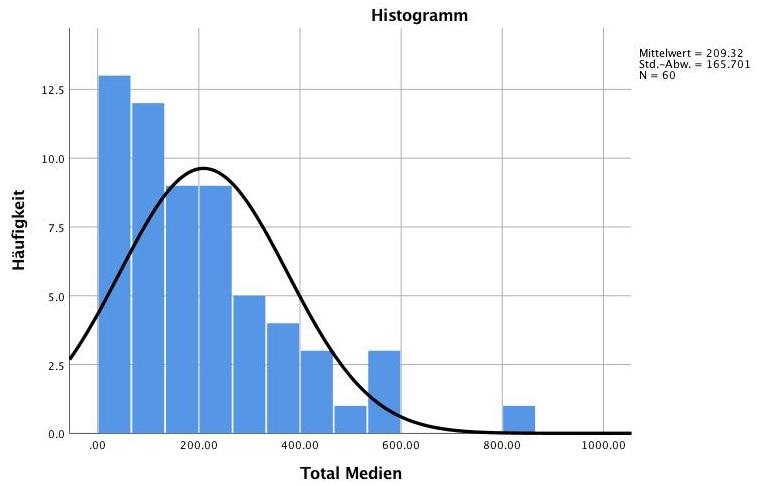
\includegraphics[scale=0.4]{content/Grafik/Histogramm_TotalMedien_SicherGebunden.jpg}
  \captionsetup{margin=80pt}
  \caption{Histogramm Mediennutzung sicher Gebundene}
  \label{fig:AppHistogrammSicherGebunden}
\end{figure}
\begin{figure}[h]
  \centering
     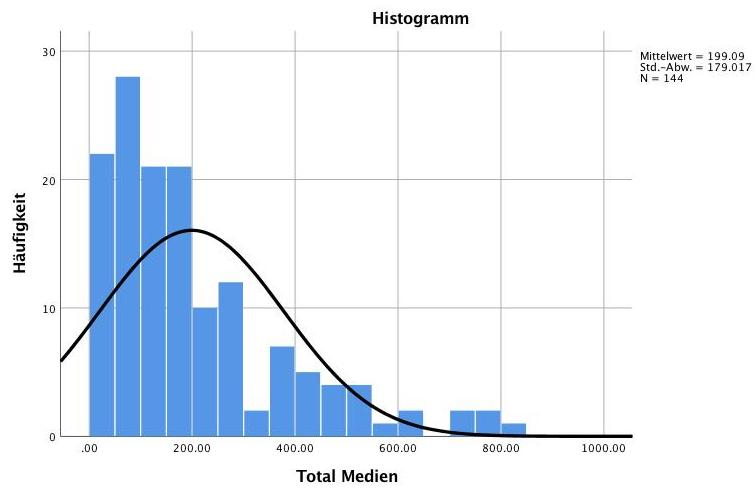
\includegraphics[scale=0.4]{content/Grafik/Histogramm_TotalMedien_UnsicherGebunden.jpg}
  \captionsetup{margin=80pt}
  \caption{Histogramm Mediennutzung unsicher Gebundene}
  \label{fig:AppHistogrammUnsicherGebunden}
\end{figure}





\newpage
\section{Q-Q-Digramme für Hypothese 1}\label{app:Hypo1_QQDiagramme}
%Q-Q-Plots
\begin{figure}[h]
  \centering
     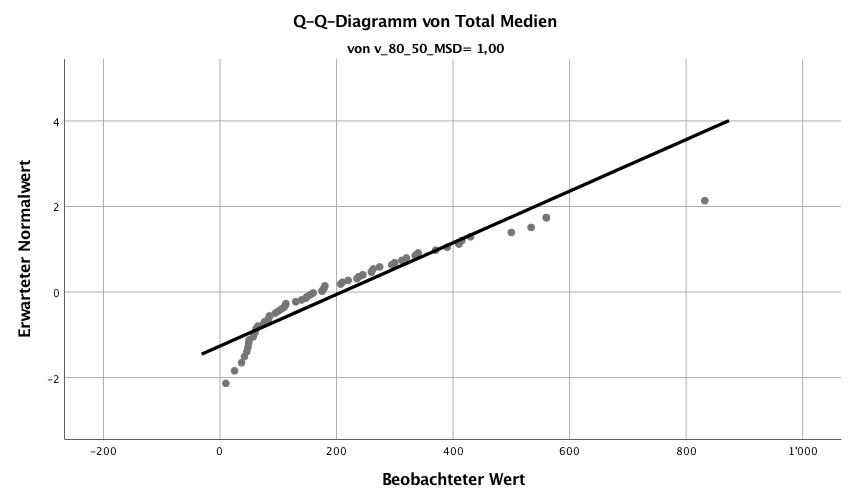
\includegraphics[scale=0.4]{content/Grafik/QQDiagramm_TotalMedien_SicherGebunden.jpg}
  \caption{Q-Q-Diagramm Mediennutzung sicher Gebundene}
  \label{fig:AppQQDiagrammSicherGebunden}
\end{figure}
\begin{figure}[h]
  \centering
     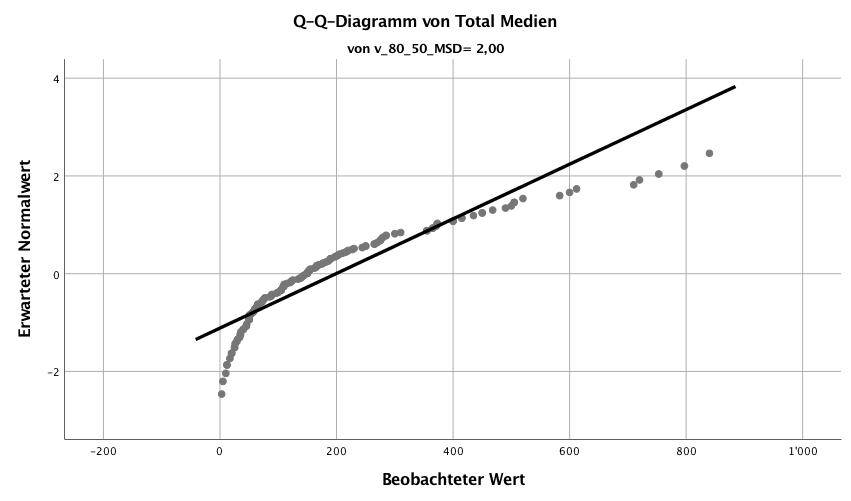
\includegraphics[scale=0.4]{content/Grafik/QQDiagramm_TotalMedien_UnsicherGebunden.jpg}
  \caption{Q-Q-Diagramm Mediennutzung unsicher Gebundene}
  \label{fig:AppQQDiagrammUnsicherGebunden}
\end{figure}
\newpage
\section{Boxplot für Hypothese 1}\label{app:Hypo1_Boxplot}
%Boxplot
\begin{figure}[h]
  \centering
     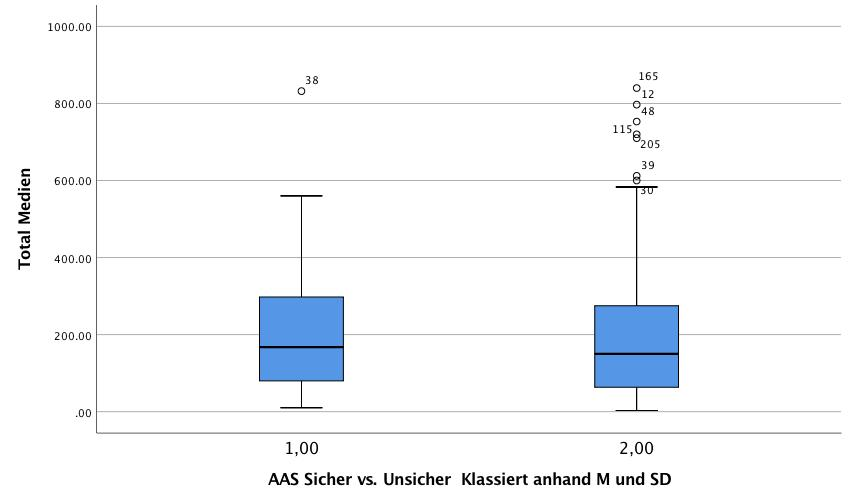
\includegraphics[scale=0.4]{content/Grafik/Boxplot_TotalMedien_SicherUnsicherGebunden.jpg}
  \caption{Boxplot Diagramm Mediennutzung unsicher vs. sicher Gebundene}
  \label{fig:AppBoxplotDiagrammSicherUnsicherGebunden}
\end{figure}
\newpage
%% Hypo 2
\section{Streudiagramme für Hypothese 2}\label{app:Hypo2_Streudiagramm}

% Streudiagramm
\begin{figure}[h]
  \centering
     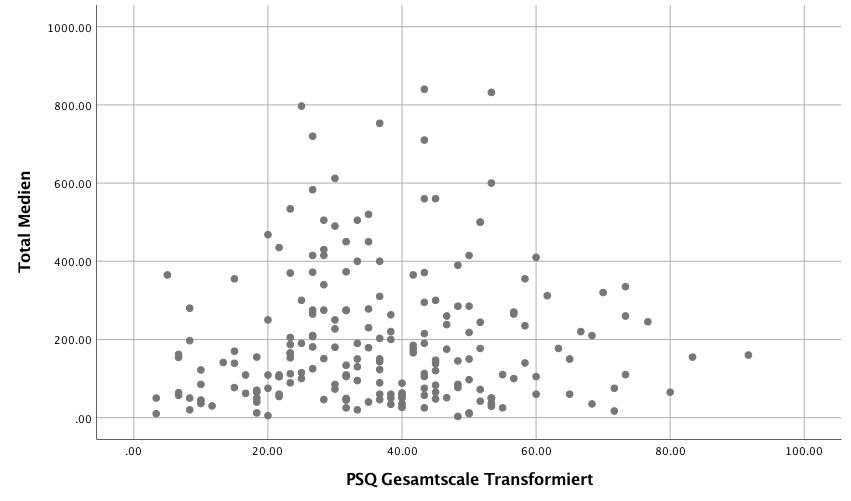
\includegraphics[scale=0.4]{content/Grafik/Streudiagramm_TotalMedien_PSQ.jpg}
  \captionsetup{margin=80pt}
  \caption{Streudiagramm Mediennutzung und Stress (PSQ)}
  \label{fig:AppStreudiagrammMedienPsq}
\end{figure}

\begin{figure}[h]
  \centering
     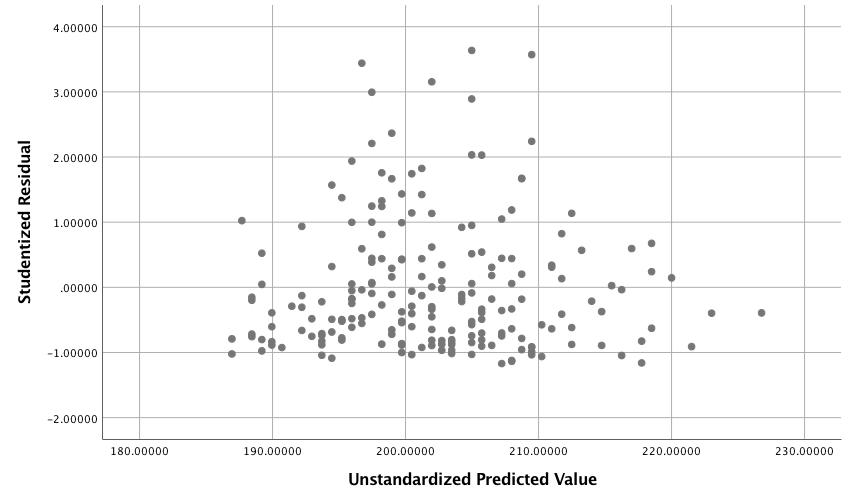
\includegraphics[scale=0.4]{content/Grafik/Streudiagramm_Hypo2_GeschaetzteWerteUndResiduen.jpg}
  \captionsetup{margin=80pt}
  \caption{Streudiagramm der Fehlerwerte  der abhängigen Variable Mediennutzung}
  \label{fig:AppStreudiagrammResiduen}
\end{figure}


\newpage
\section{Histogramm für Hypothese 2}\label{app:Hypo2_Histogramm}
\begin{figure}[h]
  \centering
     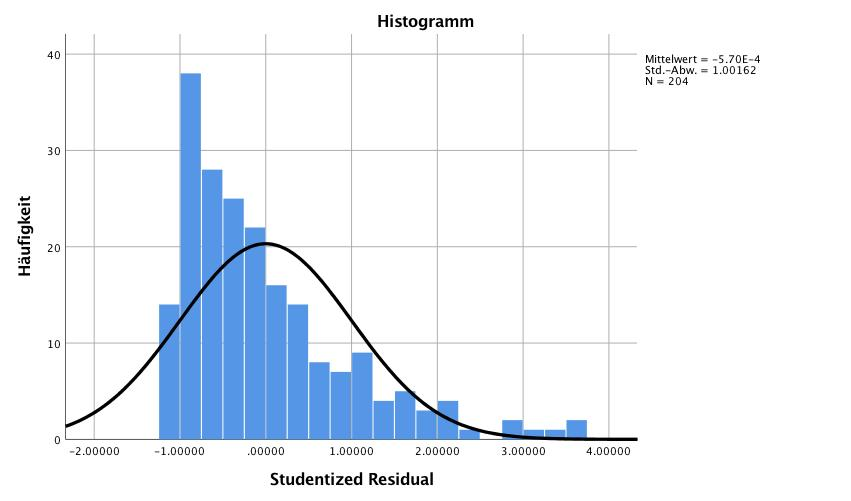
\includegraphics[scale=0.4]{content/Grafik/Histogramm_Hypo2_Residuen.jpg}
  \caption{Verteilung der Fehlerwerte}
  \label{fig:AppHistogrammResiduen}
\end{figure}
\newpage
\section{Kurvenanpassung für Hypothese 2}\label{app:Hypo2_Kurvenanpassung}
\begin{figure}[h]
  \centering
     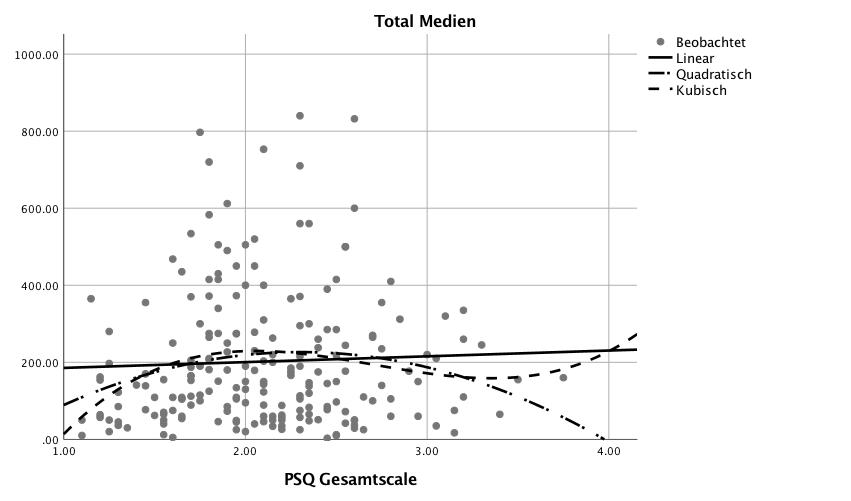
\includegraphics[scale=0.4]{content/Grafik/Streudiagramm_Hypo2_Kurvenanpassung.jpg}
  \captionsetup{margin=80pt}
  \caption{Streudiagramm Kurvenanpassung}
  \label{fig:AppHypo2StreudiagrammKurvenanpassung}
\end{figure}
\newpage
%% Hypo 3
\section{Streudiagramme für Hypothese 3}\label{app:Hypo3_Streudiagramm}
% Streudiagramm
\begin{figure}[h]
  \centering
     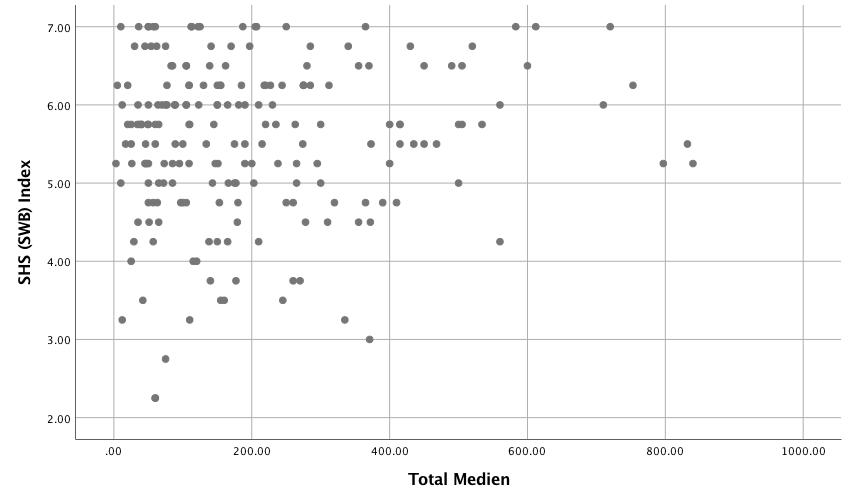
\includegraphics[scale=0.4]{content/Grafik/Streudiagramm_Hypo3.jpg}
  \captionsetup{margin=80pt}
  \caption{Streudiagramm Mediennutzung und subjektives Wohlbefinden (SHS)}
  \label{fig:AppHypo3Streudiagramm}
\end{figure}

\begin{figure}[h]
  \centering
     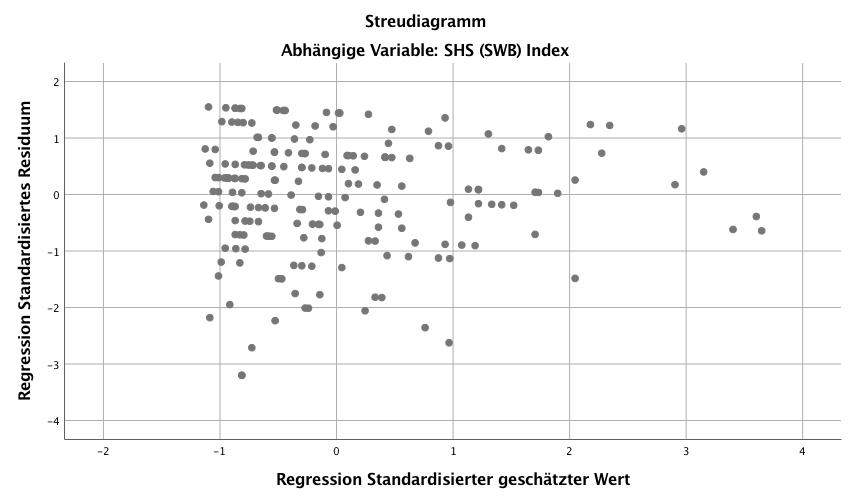
\includegraphics[scale=0.4]{content/Grafik/Streudiagramm_Hypo3_Residuen.jpg}
  \captionsetup{margin=80pt}
  \caption{Streudiagramm der Fehlerwerte  der abhängigen Variable subjektives Wohlbefinden}
  \label{fig:AppHypo3StreudiagrammResiduen}
\end{figure}
\newpage
\section{Histogramm für Hypothese 3}\label{app:Hypo3_Histogramm}
\begin{figure}[h]
  \centering
     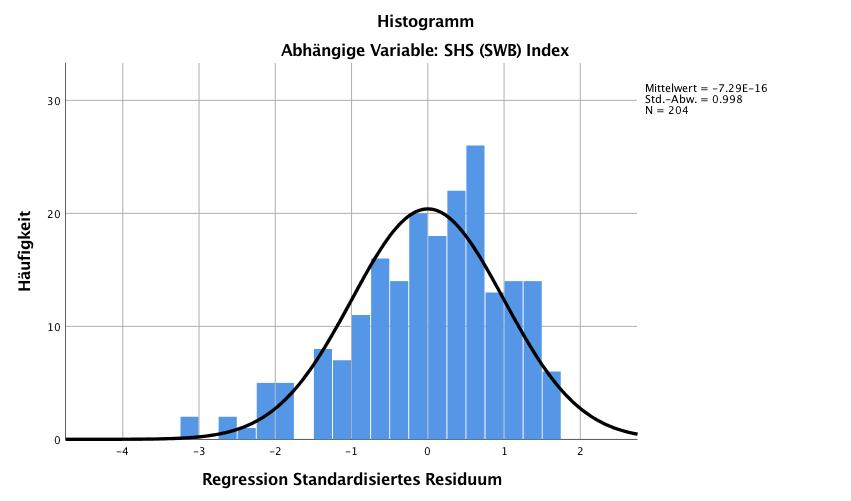
\includegraphics[scale=0.4]{content/Grafik/Histogramm_Hypo3_Normverteilung.jpg}
  \caption{Verteilung der Fehlerwerte}
  \label{fig:AppHypo3HistogrammResiduen}
\end{figure}
\newpage

% AAS Fragebogen
\section{Die Adult Attachment Scale (AAS)}\label{app:AAS}

Die im Folgenden dargestellte Adult Attachment Sacale (AAS) wurde aus der Validierungsstudie von \citeA{Schmidt2004}, des orignalen Instruments von \citeA{Collins1990} übernommen. Die Spalte \enquote{Orig.} in Tabelle \titleref{table:AASItems} beinhaltet die originale Nummerierung der Fragebogenitems. Die Spalte \enquote{Nr.} beinhaltet die neue Nummerierung, so wie sie im Umfragebogen (siehe auch \titleref{app:Fragebogen}) verwendet wurde.


\begin{table}[htbp]
\begin{tabular}{|l | m{30em} | p{2em}|} 
  \hline
  \multicolumn{3}{|c|}{\textbf{Adult Attachment Scale**}}\\
  \hline
  Nr. & Text & Orig. \\ 
  \hline\hline
  \rowcolor{lightgray}
  \multicolumn{3}{|l|}{Nähe}\\
  \hline
  02 & Es macht mich nervös, wenn mir jemand zu nahe ist.* & 03 \\
  07 & Für mich ist es schwierig, andere an mich heranzulassen.* & 08 \\
  11 & Es ist mir irgendwie unangenehm, mit anderen zu vertraut zu werden.* & 13 \\
  12 & In Freundschaften wünschen sich meine Freunde/meine Freundinnen häufig mehr Nähe von mir, als mir angenehm ist.* & 14 \\
  16 & Die Vorstellung, mir könnte jemand nahe kommen, beunruhigt mich.* & 18 \\
  \hline
  \rowcolor{lightgray} \multicolumn{3}{|l|}{Vertrauen}\\
  \hline
  01 & Ich weiß, wenn ich jemand brauche, wird auch jemand da sein. & 01 \\
  04 & Ich bin mir nicht sicher, ob ich mich immer darauf verlassen kann, dass andere da sind, wenn ich sie brauche.* & 05\\
  08 & Menschen sind nie da, wenn man sie braucht.* & 10 \\
  10 & Ich kann mich gut auf andere verlassen. & 12\\
  13 & Ich kann es mir nur schwer zugestehen, mich auf andere zu verlassen.* & 15\\
  15 & Es fällt mir schwer, anderen voll und ganz zu vertrauen.* & 17\\
  \hline
  \rowcolor{lightgray} \multicolumn{3}{|l|}{Angst}\\
  \hline
  03 & Ich mache mir oft Sorgen, dass meine Freunde/meine Freundinnen mich nicht wirklich mögen. & 04\\
  05 & Mein Wunsch, in einem anderen Menschen völlig aufzugehen, schreckt andere manchmal ab. & 06 \\
  06 & Ich merke, dass andere mich nicht so nahe an sich herankommen lassen, wie ich es gerne hätte. & 07 \\
  09 & Ich mache mir oft Sorgen, ein wichtiger Mensch könnte mich verlassen. & 11 \\
  14 & Ich mache mir oft Sorgen, dass meine Freunde/meine Freundinnen eines Tages nicht mehr mit mir befreundet sein möchten. & 16 \\
  \hline
  \multicolumn{3}{l}{* Die Items wurden für die Erstellung des Skalenwertes umcodiert.}\\
  \multicolumn{3}{l}{** Deutsche Übersetzung gemäss \citeA{Schmidt2004}}.\\
  \multicolumn{3}{l}{}\\
\end{tabular}
\caption{Items der Adult Attachment Scale}
\label{table:AASItems}
\end{table}

\newpage

% PSQ Fragebogen
\section{Perceived Stress Questionnaire (PSQ)}\label{app:PSQ}

\begin{table}[htbp]
\begin{tabular}{|p{2em} | m{30em} | l|} 
  \hline
  \multicolumn{3}{|c|}{\textbf{Perceived Stress Questionnaire}}\\
  \hline
  Nr. & Text & Orig. \\ 
  \hline\hline
  \rowcolor{lightgray}
  \multicolumn{3}{|l|}{Sorgen (worries)}\\
  \hline
  05 & Sie fürchten Ihre Ziele nicht erreichen zu können. & 09\\
  07 & Sie fühlen sich frustriert. & 12\\
  10 & Ihre Probleme scheinen sich aufzutürmen. & 15\\
  13 & Sie haben viele Sorgen. & 18\\
  15 & Sie haben Angst vor der Zukunft. & 22\\
  \rowcolor{lightgray}
  \multicolumn{3}{|l|}{Anspannung (tension)}\\
  \hline
  01* & Sie fühlen sich ausgeruht. & 01*\\
  06* & Sie fühlen sich ruhig. & 10*\\
  09 & Sie fühlen sich angespannt. & 14\\
  17 & Sie fühlen sich mental erschöpft. & 26\\
  18 & Sie haben Probleme, sich zu entspannen. & 27\\
  \rowcolor{lightgray}
  \multicolumn{3}{|l|}{Freude (joy)}\\
  \hline
  04 & Sie haben das Gefühl, Dinge zu tun, die Sie wirklich mögen. & 07\\
  08 & Sie sind voller Energie. & 13\\
  12 & Sie fühlen sich sicher und geschützt. & 17\\
  14 & Sie haben Spass. & 21\\
  16 & Sie sind leichten Herzens. & 25\\
  \rowcolor{lightgray}
  \multicolumn{3}{|l|}{Anforderungen (demands)}\\
  \hline
  02 & Sie haben das Gefühl, dass zu viele Forderungen an Sie gestellt werden. & 02\\
  03 & Sie haben viel zu tun. & 04\\
  11 & Sie fühlen sich gehetzt. & 16\\
  19* & Sie haben genug Zeit für sich. & 29*\\
  20 & Sie fühlen sich unter Termindruck. & 30\\
  \hline
  \multicolumn{3}{l}{* Bei diesen Items muss der Wert des Items von 5 abgezogen werden,}\\
  \multicolumn{3}{l}{~~~bevor das Ergebnis mit den Werten der anderen Items in die Berechnung eingeht.}\\
  \multicolumn{3}{l}{}\\
\end{tabular}
\caption{Items des Perceived Stress Questionnaire}
\label{table:PSQ}
\end{table}
\newpage

% SHS Fragebogen
\section{Subjective Happiness Scale (SHS)}\label{app:SHS}
\begin{table}[htbp]
\centering
\captionsetup{margin=5pt,skip=5pt}
\caption{Items der Subjective Happiness Scale}
\label{table:SHS}
\begin{tabular}{|p{1em} | p{4em} p{4em} p{4em} p{4em} p{4em} p{4em} p{4em}|} 
  \hline
  \multicolumn{8}{|c|}{\textbf{Subjective Happiness Scale*}}\\
  \hline
  Nr. & \multicolumn{7}{|l|}{Text}\\ 
  \hline\hline
  \rowcolor{lightgray}
  & \multicolumn{7}{|l|}{Selbstbild}\\
  \hline
  01 & \multicolumn{7}{l|}{Im Allgemeinen betrachte ich mich als:}\\
  & \multicolumn{3}{l}{Kein glücklicher Mensch} & \multicolumn{4}{r|}{Sehr glücklicher Mensch}\\
  &$\square$&$\square$&$\square$&$\square$&$\square$&$\square$&$\square$\\
  
  02 & \multicolumn{7}{l|}{Im Vergleich zu meinen Bekannten betrachte ich mich als:}\\
  & \multicolumn{3}{l}{Weniger glücklich} & \multicolumn{4}{r|}{Glücklicher}\\
  &$\square$&$\square$&$\square$&$\square$&$\square$&$\square$&$\square$\\
  
  \rowcolor{lightgray}
  & \multicolumn{7}{|l|}{Individueller Vergleich}\\
  
  03 & \multicolumn{7}{l|}{\begin{minipage}{5.8in}Manche Leute sind im Allgemeinen sehr glücklich. Sie freuen sich am Leben, unabhängig davon, wie dieses verläuft, und sie machen aus allem das Beste. Wie sehr trifft diese Charakterisierung auf Sie zu?\end{minipage}}\\
  & \multicolumn{3}{l}{Überhaupt nicht} & \multicolumn{4}{r|}{Zu einem sehr großen Teil}\\
  &$\square$&$\square$&$\square$&$\square$&$\square$&$\square$&$\square$\\
  
  04 & \multicolumn{7}{l|}{\begin{minipage}{5.8in}Manche Leute sind nicht so glücklich. Obschon sie nicht depressiv sind, schauen sie nicht so glücklich aus, wie sie sein könnten. Wie sehr trifft diese Charakterisierung auf Sie zu?\end{minipage}}\\
  & \multicolumn{3}{l}{Zu einem sehr großen Teil} & \multicolumn{4}{r|}{Überhaupt nicht}\\
  &$\square$&$\square$&$\square$&$\square$&$\square$&$\square$&$\square$\\
  \hline
  
  \multicolumn{8}{l}{* Deutsche Übersetzung gemäss \citeA{BiedaND}.}\\
  
  \multicolumn{3}{l}{}\\
\end{tabular}
\end{table}

\newpage

% Fragebogen
\section{Fragebogen}\label{app:Fragebogen}
Der im Folgenden abgebildete Fragebogen stellt eine leichte Abwandlung des originalen Onlinefragebogens dar, da die Umsetzung der grafischen Elemente zwecks Lesbarkeit in diesem Dokument vereinfacht wurden. Inhaltlich wurden keine Anpassungen vorgenommen.

\subsection{Startseite}
\textbf{Herzlich willkommen zum Elternfragebogen}

Vielen Dank, dass Sie an unserer Studie teilnehmen. Die Befragung dauert ca. 10 bis 15 Minuten. Die Daten werden vollständig anonym erfasst. Es sind keine Rückschlüsse auf einzelne Probanden möglich. Wichtig ist, dass Sie die Fragen ehrlich beantworten. Es gibt keine richtig oder falschen Antworten. Es ist kein Leistungstest. Es geht um Ihre persönliche Meinung.

Ziel dieser Arbeit ist es, die Mediennutzung von Eltern mit einem oder mehreren Kindern im Alter zwischen 0 und 1 Jahr zu erfassen. Dabei sollten Sie das Kind an mindestens zwei aufeinanderfolgenden Stunden pro Woche alleine betreuen.

Am Schluss der Umfrage haben Sie die Möglichkeit, an der Verlosung der Gutscheine (10 x CHF 50) teilzunehmen oder sich Versuchspersonenstunden (0.5 VPStunden) anrechnen zu lassen.

\begin{figure}[hbtp]
  \centering
     
\includegraphics[width=0.3\textwidth]{content/Grafik/babyRose_Logo.jpg}
  \label{fig:babyRose_Logo}
\end{figure}

Bei Fragen und Rückmeldungen zur Studie können Sie sich per Mail an Till ERNST, Stud. MSc in Applied Psychology, ernsttil@students.zhaw.ch wenden. Durch klicken von 'Weiter' bestätigen Sie, diese Informationen gelesen zu haben, und erklären sich mit der Teilnahme einverstanden.

\subsection{Demografische Daten}
Zuerst folgen ein paar Angaben zu Ihrer Person und Ihrem Kind im Alter zwischen 0 und 1 Jahr. Falls Sie mehrere Kinder in diesem Alter betreuen, entscheiden Sie sich für dasjenige, das Sie am häufigsten betreuen. Gehen Sie in den folgenden Fragen immer vom gleichen Kind aus.

\begin{longtable}[c]{ |p{1em}|p{16em}|p{16em}| }
  %\caption{Demografische Daten}\label{tab:DemografischeDaten}\\
 
  \hline
  Nr. & Frage & Antwortabstufungen \\
  \hline
  \endfirsthead
 
  \hline
  \multicolumn{3}{|c|}{ Fortsetzung Demografische Daten}\\
  \hline
  Nr. & Frage & Antwortabstufungen \\
  \hline
  \endhead
 
  \hline
  \endfoot
 
  \hline\hline
  \endlastfoot
 
  1 & Ihr Geschlecht & weiblich, männlich,  keine Angabe \\
  2 & Ihr Jahrgang & \textit{(z.B.: 1980)}  \\
  3 & Alter Ihres Kindes in Monaten & \textit{(z.B.: z.B. 5,4)}\\
  4 & Geschlecht des Kindes & weiblich, männlich, keine Angabe \\
  5 & Ihr Brutto Familieneinkommen & keine Angabe | Bis 26’000 CHF pro Jahr | Von 26’001 bis 52’000 CHF pro Jahr | Von 52’001 bis 78’000 CHF pro Jahr | Von 78’001 bis 104’000 CHF pro Jahr | 104’001 CHF pro Jahr und mehr \\
  6 & Welches ist Ihr bisher höchster Bildungsabschluss? & keine Angabe | Obligatorische Grundschule | Lehrabschluss (Sekundär II) | Berufsmatura / Fachmittelschule (Sekundär II) | Gymnasiale Maturität (Sekundär II) | Höhere Fachschule (Tertiär) | Uni / Fachhochschule (Tertiär) | Doktorat (Tertiär) \\
  7 & Wieviele Personen leben total in Ihrem Haushalt (inklusive Kinder)? & \textit{Familiengrösse} \\
  8 & Wie leben sie aktuell? & alleinstehend, verheiratet | alleinstehend, nicht verheiratet | in Partnerschaft, verheiratet | in Partnerschaft, nicht verheiratet | in einer WG, verheiratet | in einer WG, nicht verheiratet \\
  9 & An wievielen Tagen pro Woche wird Ihr Kind fremdbetreut (z.B.: durch Krippe, Hort, Nanny, Grosseltern, Tagesmutter etc.)? Sie können auch Halbtage eingeben & \textit{(z.B.: 1,5 Tage, 0 = keine Fremdbetreuung)} \\
  10 & Wie viel Prozent der Betreuung für das Kind übernehmen Sie pro Woche? & \textit{(z.B.: 50\% wenn Sie sich die Betreuung mit Ihrem Partner / Ihrer Partnerin je zur Hälfte teilen)} \\
  
\end{longtable}

\subsection{Medien und Mediennutzung}
Im Folgenden werden Sie gebeten, Angaben über verschiedene Medien-Tätigkeiten so exakt wie möglich zu machen, die Sie während der Betreuung von Ihrem Kind ausüben. Stellen Sie sich dabei die letzte Situation vor, in der Sie während mindestens zwei Stunden alleine mit Ihrem Kind waren.

Welche der folgenden Geräte und Medien haben Sie während der letzten Betreuung beruflich oder privat genutzt?

\begin{longtable}[c]{ |p{1em}|p{12em}|p{5em}|p{5em}|p{5em}|p{5em}|}
  %\caption{Demografische Daten}\label{tab:DemografischeDaten}\\
 
  \hline
  Nr. &  & privat genutzt & beruflich genutzt & privat und beruflich genutzt & nicht genutzt \\
  \hline
  \endfirsthead
 
  \hline
  \multicolumn{6}{|c|}{ Fortsetzung Medien und Mediennutzung}\\
  \hline
  Nr. &  & privat genutzt & beruflich genutzt & privat und beruflich genutzt & nicht genutzt \\
  \hline
  \endhead
 
  \hline
  \endfoot
 
  \hline\hline
  \endlastfoot
  
  
  11 & Smartphone &  &  &  &  \\
  12 & TV &  &  &  &  \\
  13 & Desktop / Laptop Computer &  &  &  &  \\
  14 & Tablet &  &  &  &  \\
  15 & Radio / Stereoanlage / CD-Player &  &  &  &  \\
  16 & Printmedien (Buch / Zeitung / Heft / Comic) &  &  &  &  \\
  17 & Foto- und/oder Videocamera &  &  &  &  \\
  18 & Spielkonsole &  &  &  &  \\
  19 & MP3 Player &  &  &  &  \\
  
\end{longtable}

Welche Medientätigkeiten in Minuten haben Sie während der letzten Betreuung im Beisein Ihres Kindes genutzt? Bitte geben Sie die Zeit in Minuten an und unterscheiden Sie, ob das Kind geschlafen hat oder wach war.
\newpage

% Mailing
\section{Mailing}\label{app:Mailing}
Das im Folgenden abgebildete Infomail diente der Rekrutierung der Stichprobe. Es handelt sich dabei um ein exemplarisches Beispiel, welches an die deutschsprachigen Elternberatungsstellen versendet wurde.

\begin{flushleft}

\textbf{Betreff:}

Auslage und Publikation für eine Eltern-Umfrage im Bereich Mediennutzung der ZHAW
\vspace{2mm}

\textbf{Inhalt:}

Sehr geehrte Damen und Herren

\vspace{2mm}
Aktuell schreibe ich eine Masterarbeit in angewandter Psychologie an der Zürcher Hochschule für Angewandte Wissenschaften (ZHAW) im Thema: Mediennutzung der Eltern im Beisein ihrer 0-1 Jahre alter Kinder.
Darin möchte ich untersuchen, ob das Medienverhalten der Eltern eine Auswirkung auf das Wohlbefinden der Eltern hat und ob das eigene Bindungsverhalten der Eltern und der aktuell empfundene Stress sich auf das Medienverhalten auswirken. 

\vspace{2mm}
Für meine Untersuchung benötige ich mindestens 280 Teilnehmer (je mehr, desto aussagekräftiger das Resultat). Da der Fragebogen für die Eltern mit etwas Aufwand und 10 bis 15 Minuten ihrer Zeit verbunden ist (alles was in dieser delikaten Zeit Mangelware ist), habe ich mittels Wettbewerb einen gewissen Anreiz für das Beantworten der Fragen geschafft (10 x 50.- bei Baby-Rose).

\vspace{2mm}
Umfragelink: https://ww2.unipark.de/uc/elternfragebogen/

\vspace{2mm}
Meine Bitte an Sie: Könnten Sie sich vorstellen diese Umfrage zu unterstützen, indem Sie diese Umfrage auf Ihrer Webseite publizieren oder Flyer in Ihrem Aushang auflegen? Dadurch würden Sie mir eine grosse Hilfe erweisen. Die Flyer würde ich Ihnen per Post zukommen lassen. Bei einer Publikation auf Ihrer Webseite ist der Medienbruch nicht so hoch (Wechsel von Analogmedium auf ein Digitales) und dadurch die Rücklaufquote etwas verbessert.
Die Umfrage wird bis Ende Mai aufgeschaltet sein.

\vspace{2mm}
Im Anhang habe ich Ihnen meine Disposition zu dieser Arbeit beigelegt, falls Sie zusätzliche Informationen zur Arbeit benötigen. Zudem habe ich Ihnen den Flyer beigelegt, den ich an diversen weiteren Fachstellen auflegen werde (Familienzentren, Mütter und Väter Beratung, etc.). 
Sollten Sie weitere Fragen haben, so werde ich Ihnen diese gerne beantworten.

\vspace{2mm}
Auf eine Rückmeldung von Ihnen freue ich mich sehr.

\vspace{2mm}
Mit besten Grüssen 

Till ERNST

Stud. MSc in angewandter klinischer Psychologie

\end{flushleft}

Zusätzlich zum Schreiben wurde dem Mailing ein Flyer angehängt. Dieser wurde auch in Papierform ausgedruckt und aufgelegt.


\begin{figure}[h]
  \centering
     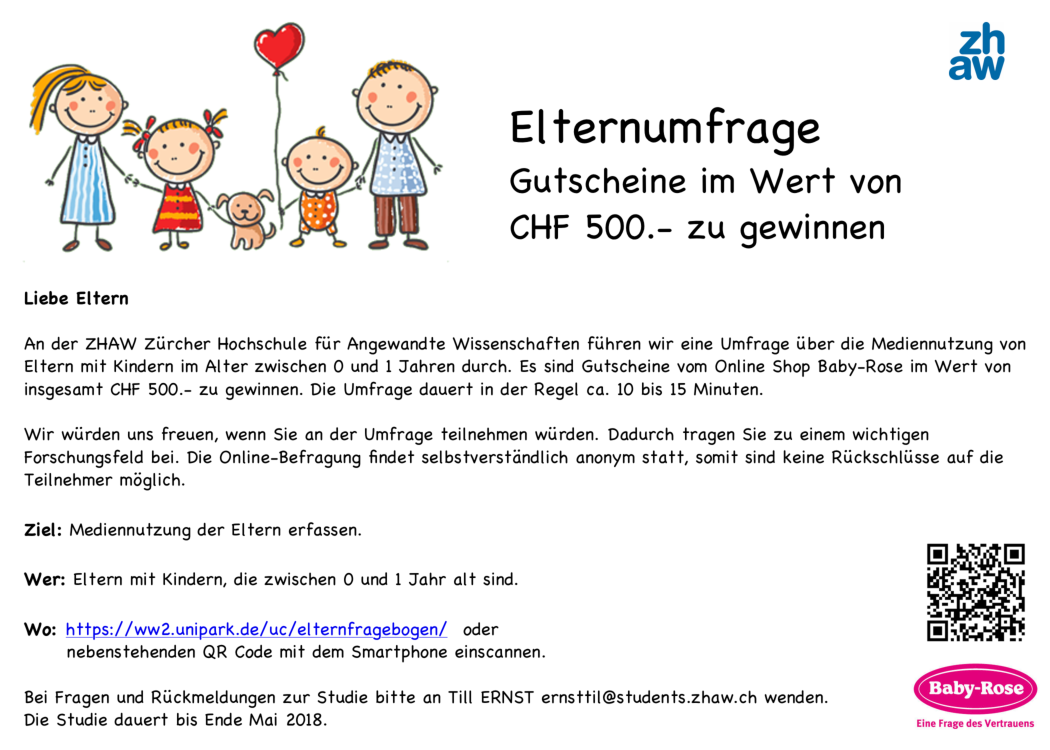
\includegraphics[scale=0.9,angle=90]{content/Grafik/Flyer_Umfrage_v2.pdf}
  \captionsetup{margin=80pt}
  \caption{Flyer für die Umfrage}
  \label{fig:flyer}
\end{figure}

\newpage

Für die Auswertung des Wettbewerbs wurden die Teilnehmer randomisiert gezogen. Unten aufgeführt ist das dazu verwendete SWIFT-Skript, die gezogenen Teilnehmer anhand ihrer ID und das versendete Gewinnerschreiben.

\subsection*{Swift 4.0 Code für die randomiesierte Ziehung}

\begin{lstlisting}
import UIKit
for i in 0 ..< 10 {
    print ("Gewinner \(i)", arc4random_uniform(159))
}
\end{lstlisting}

Dabei ist zu beachten dass $N$=159 beim Wettbewerb mitgemacht haben.

\subsection*{Gewinner anhand Personen-ID}
\begin{itemize}
    \item Gewinner 0: 20
    \item Gewinner 1: 147
    \item Gewinner 2: 124
    \item Gewinner 3: 4
    \item Gewinner 4: 114
    \item Gewinner 5: 35
    \item Gewinner 6: 86
    \item Gewinner 7: 106
    \item Gewinner 8: 64
    \item Gewinner 9: 154
\end{itemize}

\subsection*{Mailing an Gewinner}
\begin{flushleft}
\textit{Betreff:}
Sie haben bei der Elternumfrage gewonnen

\textit{Inhalt:}
Liebe Gewinnerin, lieber Gewinner

Vor einiger Zeit haben Sie an der Elternumfrage meiner Masterarbeit der ZHAW teilgenommen. Vielen Dank dafür. 

Sie wurden als glückliche Gewinnerin/Gewinner ausgewählt und erhalten einen Gutschein im Wert von CHF 50.- des online Shops Baby-Rose.

Dazu bitte ich Sie, mir Ihre vollständige Postanschrift zukommen zu lassen, damit ich Ihnen via Baby-Rose den Gutschein aushändigen kann.

Vielen Dank und beste Grüsse

Till ERNST
\end{flushleft}
\newpage

% Flyer für die Rekrutierung
\section{Flyer}\label{app:Flyer}
\begin{figure}[h]
  \centering
     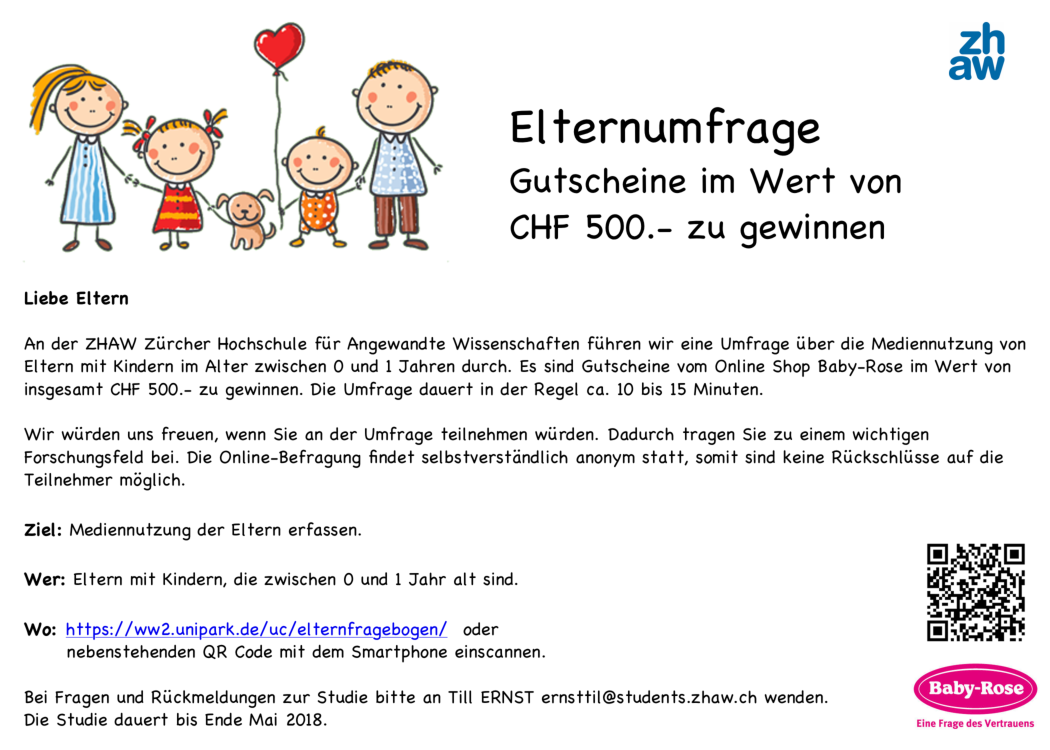
\includegraphics[scale=0.9,angle=90]{content/Grafik/Flyer_Umfrage_v2.pdf}
  \caption{Flyer für die Umfrage}
  \label{fig:flyer}
\end{figure}
\newpage

% Rekrutierung
\section{Rekrutierung}\label{app:Rekrutierung}
Alle angeschriebenen Institutionen werden in folgenden Tabellen aufgeführt:
\begin{itemize}
    \item \textit{Tabelle \ref{table:AppRekrutierungElernebratungsstellen} \nameref{table:AppRekrutierungElernebratungsstellen}}
    \item \textit{Tabelle \ref{table:AppRekrutierung} \nameref{table:AppRekrutierung}}
\end{itemize}


%Table Elternberatungsstellen
\begin{longtable}[htbp]{|p{0.2em} p{20em} | c | c |} 
  \caption{Elternberatungsstellen} \label{table:AppRekrutierungElernebratungsstellen}\\
  \hline
  \rowcolor{lightgray}
  \multicolumn{4}{|l|}{Elternberatungsstellen via Fachverband Mütter und Väterberatung \cite{Sfmvb2018a}}\\
  \hline
  \multicolumn{2}{|l|}{Institution und Adresse} & Anfrage & Verteilung\\
  & & (Mail / Tel. / Priv.) & (HP / FB / Flyer)\\
  \hline
  \endfirsthead
 
  \hline
  \rowcolor{lightgray}
  \multicolumn{4}{|c|}{ Fortsetzung Elternberatungsstellen}\\
  \hline
  \multicolumn{2}{|l|}{Insititution und Adresse} & Anfrage & Verteilung\\
  & & (Mail / Tel. / Priv.) & (HP / FB / Flyer)\\
  \hline
  \endhead
 
  \hline
  \endfoot
 
  \hline\hline
  \endlastfoot
  
  
  \multicolumn{2}{|l|}{Sektion Aargau (info@mvb-aargau.ch)} & Mail & HP, FB\\
  & Bezirk Rheinfelden (info@muebe.ch) & Mail & k.R.\\
  & Bezirk Laufenburg (mvb@gvlfbg.ch) & Mail & k.R.\\
  & Zofingen Regio (susanne.breitenstein@zofingenregio.ch) & Mail & HP, Flyer \\
  & MVB Aarau plus (info@mvb-aarauplus.ch) & Mail & HP, Flyer \\
  & Bezirk Kulm ( mvb.kulm@sharknet.ch) & Mail & Flyer\\
  & Bezirk Brugg (soziale.dienstleistungen-mvb@brugg.ch) & Mail & k.R.\\
  & Bezirk Baden (office@mvb-baden.ch ) & Mail & k.R. \\
   \multicolumn{2}{|l|}{Appenzell Ausserhoden } & Mail & Nein\\
  & (Kontaktformular http://www.projuventute-ar.ch/ ) & & \\
  \multicolumn{2}{|l|}{Appenzell Innerhoden } & Mail & Flyer\\
  & (info@spitexai.ch) & & \\
  \multicolumn{2}{|l|}{Basel Land} & & k.R.\\
  & (rgbeiderbasel@gmx.ch) & & \\
  \multicolumn{2}{|l|}{Basel Stadt} & Mail & Flyer\\
  & (info@elternberatungbasel.ch) & & \\
  \multicolumn{2}{|l|}{Sektion Bern (geschaeftsleitung@mvb-be.ch)} & Mail & k.R.\\
  & Bezirk Bern Mittellan (karin.messikommer@mvb-be.ch) & Mail & k.R. \\
  & Bezirk Emmental–Oberaargau (emmental-oberaargau@mvb-be.ch) & Mail & k.R. \\
  & Bezirk Jura (jurabernois-seeland@mvb-be.ch) & Mail & Nein \\
  & Bezirk Oberland (oberland@mvb-be.ch) & Mail & k.R. \\
  \multicolumn{2}{|l|}{Freiburg Seebezirk} & Mail & k.R.\\
  & (info@mvbsee.ch) & & \\
  \multicolumn{2}{|l|}{Freiburg Sensebezirk} & Mail & k.R.\\
  & (muetterberatung@spitexsense.ch) & & \\
  \multicolumn{2}{|l|}{Sektion St Gallen} &  & \\
  & Sarganserland (mvbs@bluewin.ch) & Mail & k.R.\\
  & See-Gaster (barbara.oberkalmsteiner@hotmail.ch) & Mail & k.R.\\
  & Rapperswil-Jona (Kontaktformular) & Mail & k.R.\\
  & Region St.Gallen (info@ovk.ch) & Mail & Flyer\\
  & Region Mittleres und Oberes Rheintal (mvb@s-d-m.ch) & Mail & Flyer\\
  & Toggenburg (mvb.obertoggenburg@thurweb.ch) & Mail & Flyer\\
  & Untertoggenburg-Wil-Gossau (Kontaktformular) & Mail & Flyer\\
  \multicolumn{2}{|l|}{Sektion Glarus} &  & \\
  & Glarus Nord (marianne.blaser@muevaeberatung.ch ) & Mail & k.R.\\
  & Glarus Mitte (rebecca.feldmann@muevaeberatung.ch) & Mail & HP, Flyer\\
  & Glarus Süd (sabine.haemmerli@muevaeberatung.ch) & Mail & k.R.\\
  \multicolumn{2}{|l|}{Sektion Graubünden ( info@kjbe.ch)} & Mail & Flyer\\
  \multicolumn{2}{|l|}{Sektion Kt Luzern} & & \\
  & Stadt Luzern und Umgebung (mvb@stadtluzern.ch) & Mail & Flyer\\
  & Gemeinden im Einzugsgebiet Amt Willisau (willisau(at)sobz.ch) & Mail & k.R.\\
  & Gemeinden im Einzugsgebiet Amt Hochdorf und Amt Sursee (hochdorf(at)sobz.ch) & Mail & k.R.\\
  & Ganzes Amt Entlebuch, Wohlhusen und Ruswil (info(at)sobz-entlebuch.ch) & Mail & k.R.\\
  & Buchrain, Ebikon, Dierikon, Gisikon, Honau und Root (mvb@ebikon.ch) & Mail & Flyer\\
  \multicolumn{2}{|l|}{Sektion Obwalden (info@spitexow.ch)} & Mail & Flyer\\
  \multicolumn{2}{|l|}{Sektion Nidwalden (muevae@spitexnw.ch)} & Mail & Flyer\\
  \multicolumn{2}{|l|}{Sektion Schaffhausen (anne.forster(at)stsh.ch)} & Mail & Flyer\\
  \multicolumn{2}{|l|}{Sektion Schwyz (mvb@spitex-schwyz.ch )} & Mail & Flyer\\
  \multicolumn{2}{|l|}{Sektion Solothurn} &  & \\
  & info@muetterberatung-so.ch & Mail & k.R.\\
  & mvb@srun.ch & Mail & Flyer\\
  & claudia.starling@arkadis.ch & Mail & Flyer\\
  & c.fuerst@zsth.ch & Mail & k.R.\\
  & muva@sozialregion.ch & Mail & k.R.\\
  & muva.kuenzli@hotmail.ch & Mail & k.R.\\
  & muva.grenchen@bluewin.ch & Mail & Flyer\\
  & margrit.bianchi@arkadis.ch & Mail & k.R.\\
  & muva.marolf@outlook.com & Mail & k.R.\\
  & m.bohren@mvb-so.ch & Mail & k.R.\\
  & m.meyer@zsth.ch & Mail & k.R.\\
  & m.schibli@mvb-so.ch & Mail & k.R.\\
  & regina.willener@arkadis.ch & Mail & k.R.\\
  & muva.tschumi@hotmail.ch & Mail & k.R.\\
  & muva.bigler@hotmail.ch & Mail & k.R.\\
  & v.anliker@mvb-so.ch & Mail & k.R.\\
  & vreni.studer@sunrise.ch  & Mail & k.R.\\
  \multicolumn{2}{|l|}{Sektion Thurgau (info@perspektive-tg.ch)} &  & Flyer\\
  & Region Arbon (mvb-arbon@perspektive-tg.ch) & Mail & k.R.\\
  & Diessenhofen (mvb-diessenhofen@perspektive-tg.ch ) & Mail & k.R.\\
  & Frauenfeld (mvb-frauenfeld@perspektive-tg.ch) & Mail & k.R.\\
  & Kreuzlingen (mvb-kreuzlingen@perspektive-tg.ch) & Mail & k.R.\\
  & Münchwilen (mvb-muenchwilen@perspektive-tg.ch) & Mail & Flyer.\\
  & Romanshorn (mvb-romanshorn@perspektive-tg.ch ) & Mail & k.R.\\
  & Weinfelden (mvb-weinfelden@perspektive-tg.ch) & Mail & k.R.\\
  & Amrsiwil Bischofzell (mvb(at)conexfamilia.ch) & Mail & k.R.\\
  \multicolumn{2}{|l|}{Sektion Uri (info@spitexuri.ch)} & Mail & Flyer\\
  \multicolumn{2}{|l|}{Sektion Wallis} & &\\
  & Oberwallis Region Goms, Brigerberg (info@smzo.ch) & Mail & Flyer\\
  & Unterwallis (info@cms-smz-vs.ch, info.brig@smzo.ch ) & Mail & k.R.\\
  \multicolumn{2}{|l|}{Sektion Zug (mail@punkto-zug.ch)} & Mail & k.R.\\
  & Baar - s.stucki@punkto-zug.ch & Mail & k.R.\\
  & Cham - s.dober@punkto-zug.ch & Mail & k.R.\\
  & Hünenberg - n.fink@punkto-zug.ch & Mail & k.R.\\
  & Menzingen - c.sgier@punkto-zug.ch & Mail & k.R.\\
  & Oberägeri - k.bernheim@punkto-zug.ch & Mail & k.R.\\
  & Rotkreuz - c.sgier@punkto-zug.ch & Mail & k.R.\\
  & Stadt Zug - u.stucky@punkto-zug.ch & Mail & k.R.\\
  \multicolumn{2}{|l|}{Sektion Zürich} &  & \\
  & Kleinkindberatung Stadt Zürich (Denise.Ernst@zuerich.ch, mvb@zuerich.ch) & Mail & Flyer\\
  & Albisrieden - Ursula.Zatti-Schwyzer@zuerich.ch & Mail & k.R.\\
  & Altstetten - Verena.Keller@zuerich.ch & Mail & k.R.\\
  & Hard - Carola.Bloch@zuerich.ch & Mail & Flyer\\
  & Wiedikon - Leila.Aniba@zuerich.ch & Mail & k.R.\\
  & Industrie - Christiane.Flach@zuerich.ch & Mail & k.R.\\
  & Oerlikon - Simone.MeyerGuengoer@zuerich.ch & Mail & k.R.\\
  & Affoltern - Loraine.Reiner@zuerich.ch & Mail & k.R.\\
  & Seebach - Gabriele.Franz@zuerich.ch & Mail & k.R.\\
  & Schwamendingen  - Barbara.Imbach@zuerich.ch & Mail & k.R.\\
  & Enge - Sandra.Eugster@zuerich.ch & Mail & k.R.\\
  & Wollishofen - Daniela.Gilli@zuerich.ch & Mail & k.R.\\
  & Wiedikon - Loredana.Francescotto@zuerich.ch & Mail & k.R.\\
  & Seefeld - Astrid.Raes@zuerich.ch & Mail & k.R.\\
  & Witikon -  Eliane.Wirth@zuerich.ch & Mail & k.R.\\
  & Milchbuck - Martina.Schmid@zuerich.ch & Mail & Flyer\\
  & Wipkingen - Arlette.Rutschmann@zuerich.ch & Mail & k.R.\\
\end{longtable}


%Table
\begin{longtable}[htbp]{|p{0.2em} p{20em} | c | c |} 
  \caption{Stichprobengewinnung} \label{table:AppRekrutierung}\\
  
  \rowcolor{lightgray}
  \multicolumn{4}{|l|}{Elternberatungsstellen via Fachverband Mütter und Väterberatung \cite{Sfmvb2018a}}\\
  \hline
  \multicolumn{2}{|l|}{Insititution und Adresse} & Anfrage & Verteilung\\
  & & (Mail / Tel. / Priv.) & (HP / FB / Flyer)\\
  \hline
  \endfirsthead
 
  \hline
  \rowcolor{lightgray}
  \multicolumn{4}{|c|}{ Fortsetzung Elternberatungsstellen}\\
  \hline
  \multicolumn{2}{|l|}{Insititution und Adresse} & Anfrage & Verteilung\\
  & & (Mail / Tel. / Priv.) & (HP / FB / Flyer)\\
  \hline
  \endhead
 
  \hline
  \endfoot
 
  \hline\hline
  \endlastfoot
  
  
  \multicolumn{2}{|l|}{Sektion Aargau (info@mvb-aargau.ch)} & Mail & HP, FB\\
  & Bezirk Rheinfelden (info@muebe.ch) & Mail & k.R.\\
  
\end{longtable}
\newpage

% Wettbewerb
\section{Wettbewerb}\label{app:Wettbewerb}
\subsection*{Swift 4.0 Code für die randomiesierte Ziehung}

\begin{lstlisting}
import UIKit
for i in 0 ..< 10 {
    print ("Gewinner \(i)", arc4random_uniform(159))
}
\end{lstlisting}

Dabei ist zu beachten dass $N$=159 beim Wettbewerb mitgemacht haben.

\subsection*{Gewinner anhand Personen-ID}
\begin{itemize}
    \item Gewinner 0: 20
    \item Gewinner 1: 147
    \item Gewinner 2: 124
    \item Gewinner 3: 4
    \item Gewinner 4: 114
    \item Gewinner 5: 35
    \item Gewinner 6: 86
    \item Gewinner 7: 106
    \item Gewinner 8: 64
    \item Gewinner 9: 154
\end{itemize}

\subsection*{Mailing an Gewinner}
\begin{flushleft}
\textit{Betreff:}
Sie haben bei der Elternumfrage gewonnen

\textit{Inhalt:}
Liebe Gewinnerin, lieber Gewinner

Vor einiger Zeit haben Sie an der Elternumfrage meiner Masterarbeit der ZHAW teilgenommen. Vielen Dank dafür. 

Sie wurden als glückliche Gewinnerin/Gewinner ausgewählt und erhalten einen Gutschein im Wert von CHF 50.- des online Shops Baby-Rose.

Dazu bitte ich Sie, mir Ihre vollständige Postanschrift zukommen zu lassen, damit ich Ihnen via Baby-Rose den Gutschein aushändigen kann.

Vielen Dank und beste Grüsse

Till ERNST
\end{flushleft}
\newpage

% Ehrenwörtliche Erklärung

\includepdf{content/PDF/EhrenwSigned.pdf}

\end{document}

%
% Please see the package documentation for more information
% on the APA6 document class:
%
% http://www.ctan.org/pkg/apa6
%